% Hauptdatei
% **********

\documentclass[a4paper,oneside,12pt]{article}

% a4paper steht f�r die Papiergr��e
% oneside steht f�r einseitigen Druck (twoside steht f�r zweiseitigen Druck)
% 12pt steht f�r die Standardschriftgr��e


% --------------------------------------------------------------------

% Standardpakete
% **************

% sprachspezifische Anpassungen
% -----------------------------

\usepackage[english,ngerman]{babel}

% Seitenlayout
% ------------

\usepackage[a4paper, driver=pdftex]{geometry}
\geometry
{% siehe geometry.pdf auf Seite 4 (Figure 1)
	left=3cm,
	right=3cm,
	bottom=3cm,
	top=3cm,
	%showframe=true, %Rahmen anzeigen lassen (auf erster Seite)
	headheight=2cm,
	headsep=0.5cm,
	footskip=1cm,
	% zus�tzlicher Rand f�r Bindung
	bindingoffset=0cm
}

% Kodierung und Schriften
% -----------------------

% Zeichenkodierung
\usepackage[latin1]{inputenc}
\usepackage[T1]{fontenc}

% Das Paket `helvet' legt `Helvetica' als serifenlose Schrift fest
% Das Paket `courier' legt `Courier' als Schreibmaschinenschrift fest.
\usepackage[scaled=1]{helvet}
\usepackage{courier}

% alternativ - �hnlich der LaTeX-StabdardschrifrStandardschrift Computer Modern (unterst�tzt Zeichen mit Akzenten etc. besser)
%\usepackage{lmodern}


% You may notice that LaTeX�s standard font (Computer Modern) is only available OT1-encoded (TeX�s standard). This makes TeX spit out ugly bitmapped fonts with T1 encoding by default.
% To overcome this, you could load the alternative Latin Modern Fonts (LM) which have been created as an extension of the CM for (not only) all sort of accented characters.
% Hence, try out to have TeX nicely typeset accented characters.
% http://www.win.ua.ac.be/~nschloe/content/top-10-latex-modules

% kleine typografische Anpassungen - nicht wichtig, sieht aber besser aus
% -----------------------------------------------------------------------

\usepackage{microtype}

% Physikalische Einheiten einfach verwenden
% Einheiten werden im Text- und Mathematikmodus aufrecht gesetzt.
% Im Textmodus wird die Formatierung des restlichen Text �bernommen (fett etc.)
\usepackage{units}

%Beispiele:
%\unit[1]{m}
%\unitfrac[1]{m}{s}
%\nicefrac{m}{s}

% Mathe
% -----

% verbessertes Mathezeugs

% This package defines commands to access bold math symbols. The basic command
% is \bm which may be used to make the math expression in its argument be typeset
% using bold fonts. The syntax of \bm is: %\bm{math expression}
\usepackage{amsmath, amssymb, bm}

% Erweitert amsmath und behebt einige Bugs
\usepackage[fixamsmath,disallowspaces]{mathtools}

% Warnt bei Benutzung von Befehlen die mit amsmath inkompatibel sind.
\usepackage[all,warning]{onlyamsmath}

% aufrechte griechische Buchstaben: \upmu etc.
\usepackage{upgreek}

% Zitate - This package provides advanced facilities for inline and display quotations
\usepackage[]{csquotes}

% Farben verwenden
\usepackage{xcolor}

% bessere Unterst�tzung von Gleitumgebungen
\usepackage{float}
\floatplacement{figure}{H} %wenn nix anderes dran steht, dass wird das Objekt HIER platziert

% Beschriftung von Tabellen, Abbildungen etc. beeinflussen, am besten Doku dazu lesen:
% http://www.math.ntnu.no/~berland/latex/docs/caption.pdf
% nach float, rotating und subfigure!
% normal                provides `normal' captions, this is the default
% hang or isu           provides captions with hanging indention
% center                provides captions where each line is centered
% centerlast            provides captions where the last line of the
%                       paragraph is centered
% nooneline             if a caption ts on one line on the page,
%                       it will be centered. If you don't like this
%                       behaviour, just select this option.
% scriptsize...Large    sets the font size of the captions
% up, it, sl, sc,
% md, bf, rm, sf,
% or tt                 sets the font attribute of the caption labels.
% ruled                 supports ruled floats of the float package, see
%                       section 1.1 for details
\usepackage[hang,small,bf]{caption}
    \renewcommand{\captionfont}{\sffamily}
    \renewcommand{\captionlabelfont}{\sffamily\bfseries}



% Einbindung von Grafiken (pdf, png, jpg)
% siehe LaTeX-Begleiter, Auflage 2 ab Seite 636.
\usepackage[pdftex]{graphicx}

% Es stellt das Symbol der europ�ischen W�hrung, des Euro, in LaTeX zur Verf�gung.
% Die Spezifikation stammt aus dem c't-Magazin 11/98, Seite 211, und aus der Encyclopaedia Britannica, Book of the Year 2002.
% http://www.theiling.de/eurosym.html
% http://www.ctan.org/tex-archive/fonts/eurosym/
\usepackage{eurosym}
\DeclareInputText{128}{\euro} % ANSI code for euro: � \usepackage{eurosym}

% Standardpfad f�r Grafiken definieren, siehe LaTeX-Begleiter auf Seite 642 ff.
\graphicspath{{./03_Grafiken/}}


% Symbole
% *******


% alle Symbole siehe 98_Sonstiges/symbols-a4.pdf

% -------------------------------------------------------
% textcomp-Paket
% Das Erg�nzungspaket textcomp stellt verschiedene Symbole f�r den Textmodus
% bereit (mathcomp analog f�r Mathematikmodus).
% Es baut auf den EC-Schriften auf (hier: cmr).
% Verwendet man andere Schriften, so stehen nicht alle Symbole zur Verf�gung.

% Mit der Paket-Option force kann man erwzingen, dass Zeichen immer ausgegeben werden,
% auch wenn die Gefahr besteht, dass das Symbol in der Schriftart nicht verf�gbar ist
% -> man bekommt dann evtl. ein gef�lltes Viereck

% Oder besser:  [force,almostfull].  Im Gegensatz zu [force] alleine
% werden dann wenigstens diejenigen Zeichen automatisch durch CM
% ersetzt, die in nicht-CM-Fonts so gut wie immer fehlen, n�mlich
% \t und \textcircled.

% Symbole:      98_Sonstiges/textcomp.pdf
% Hinweise:     98_Sonstiges/textcomptst.pdf

\usepackage{textcomp}
\usepackage{mathcomp}
% Textmodus:        \textleaf
% Mathematikmodus:  $\tcleaf$
% -------------------------------------------------------

% -------------------------------------------------------
% marvosym-Paket - vertr�gt sich nicht mit dem textcomp-Paket: entweder oder

% Weitere Symbole

% Doku: 98_Sonstiges/marvodoc.pdf

% Paket �berschreibt den Mathematik-Befehl "\Rightarrow" -> nachfolgend ein Workarround, um den urspr�nglichen Befehl zu "retten".

% \let\OldRightarrow\Rightarrow % alte Bedeutung retten
% \usepackage{marvosym} %\Rightarrow wird umdefiniert
% \let\Rightarrow\OldRightarrow % alte Bedeutung wird restauriert.

% \let: Low-Level-TeX-Anweisung um einem Makro die Definition eines anderen Makros zuzuweisen. 
%--------------------------------------------------------

% Weitere Pakete: wasysym, pifont, latexsym
% Kopf_und_Fusszeile
% ******************

\usepackage[]{fancyhdr}

% Kopfzeile
% ---------

\lhead{Hochschule Esslingen \\Technische Informatik}
\chead{}
\rhead{Alexander Stoltz \\ Benjamin Jai�le}

% Optional
% --------

% Kopfzeile rechts, linksb�ndig ausgerichtet
% siehe Begleiter auf Seite 233, Bsp. 4-1-3
%\rhead{\begin{tabular}[b]{l@{}}
%lala: lalalalala\\
%lalala: lala
%\end{tabular}
%}

% Fu�zeile
% --------

\lfoot{6. semester}
\cfoot{\thepage}
\rfoot{Research paper}

% Linienbreiten definieren
% ------------------------

\renewcommand\headrulewidth{0.4pt}
\renewcommand\footrulewidth{0.4pt}

% coolere Kopfzeile
% -----------------

% siehe LateX Begleiter S. 235 und 233
%\renewcommand\headrule
%{
%{\color{blue}%
%\hrule height 2pt width\headwidth
%\vspace{1pt}%
%\hrule height 1pt width\headwidth
%\vspace{-2pt}} %standardm��ig gibt es zwischen Kopfzeile und Text einen Abstand von \baselineskip
%}

% Farbdefinitionen
% ****************

% siehe z. B. http://www.olos.de/~ukern/publ/tex/pdf/dtk200402.pdf
% ----------------------------------------------------------------

\xdefinecolor{myBlue1}{RGB}{0,0,255}  %0..255
\xdefinecolor{myBlue2}{rgb}{0,0,1}    %0..1
\xdefinecolor{myGray}{gray}{0.2}    %0..1
% Spezialpakete
% *************

% Kommentar-Umgebung
% ------------------

% Wenn als optionales Argument myComment drin steht, dann wird die entsprechende Umgebumg im Code eingebunden -    ansonsten nicht.

% aktiviert:
\usepackage[myComment]{optional}

% deaktiviert:
% \usepackage[NotmyComment]{optional}

% Verwendung im Code:
% \opt{myComment}{Kommentar - wie z. B.: Hier fehlt noch ein Bild}

% --------------------------------------------------------------------------------------

% Blindtext zum Testen von Textausgaben
\usepackage{blindtext}

% bessere Unterst�tzung der ref-Befehle - siehe LaTeX-Begleiter ab Seite 72 (2. Auflage)
\usepackage[ngerman]{varioref}
\newcommand\eqvref[1]{\eqref{#1}\ \vpageref{#1}}

% Kann verwendet werden um bei Makros ohne Argument korrekte Leerzeichen folgen
% siege LaTeX Begleiter Seite 86 f., 2. Auflage
\usepackage{xspace}


% Verwenden von URLs im Text
% Latex-Begleiter auf Seite 100 f., 2. Auflage
% hyphens-Option: Umbruch auch an Bindestrichen erlaubt, sonst nur an // , Doppelpunkten und Punkten
\usepackage[hyphens]{url}
% Stil der Link-Formatierung festlegen - kann auch im Text neu ge�ndert werden!
% tt (Typewriter), rm (Roman), sf (Sans Serif), same (wie restlicher text)
\urlstyle{tt}

% Programmcode einbinden
% ----------------------

\usepackage{listings}
\lstset{language=Matlab}
\lstset{%
backgroundcolor=\color{myListingBackground},
basicstyle=\ttfamily,
keywordstyle=\ttfamily\color{myListingKeyword},
commentstyle=\ttfamily\color{myListingComment},
identifierstyle=, % nothing happens
stringstyle=\ttfamily\color{myListingStrings},
showstringspaces=false,
breaklines=true,
breakautoindent=true
numberblanklines=true,
numberstyle=\scriptsize\color{black}\sffamily,
tabsize=3,
numbers=left
} % no special string spaces

% Farbdefinitionen speziell f�r Listings
%\xdefinecolor{myListingGreen}{RGB}{23,23,255}  %0..255

\xdefinecolor{myListingComment}{RGB}{34,139,34}
\xdefinecolor{myListingBackground}{rgb}{0.9,0.9,0.9}
\xdefinecolor{myListingKeyword}{rgb}{0,0.1,0.8}
\xdefinecolor{myListingStrings}{RGB}{160,32,240}

%Zeilenabstand in Aufz�hlungen kleiner
\usepackage{mdwlist}

 % hier kann man auch \myComment deaktivieren
% Absaetze
% ********

% Absatz-Einr�ckung festlegen
% ---------------------------

\setlength{\parindent}{0em}

% Abstand zwischen zwei Abschnitten festlegen
% -------------------------------------------

\setlength{\parskip}{1em}

% Ueberschriften_und_Inhaltsverzeichnis
% *************************************


% Nummerierung der �berschriften bis zur Ebene 5
\setcounter{secnumdepth}{5}
% oder eben bis zur vierten Ebene...
%\setcounter{secnumdepth}{4}

% Mit diesem Befehl wird die die Tiefe des Inhaltsverzeichnisses ausgew�hlt.
\setcounter{tocdepth}{4}


% �berschriften der Ebene 4 und 5 (paragraph und subparagraph) abgesetzt formatieren:
% Der nachfolgende Text beginnt also in einer neuen Zeile - ist standardm��ig nicht der Fall
% Quelle(n):
% 1. http://www.zdv.uni-tuebingen.de/static/skripte/tech/tech_skript_f.pdf
% 2. LaTeX-Begleiter, z. B. auf Seite 32 (2. Auflage)
% ----------------------------------
\makeatletter
\renewcommand\paragraph{\@startsection
{paragraph}{4}{0em}                                % {Name}{Ebene}{Einzug}
{\baselineskip}{.2\baselineskip}                   % {vor-Abstand}{nach-Abstand}
{\normalsize\bfseries}}                            % {Layout}
\makeatother
% ----------------------------------
\makeatletter
\renewcommand\subparagraph{\@startsection
{subparagraph}{5}{0em}                              % {Name}{Ebene}{Einzug}
{\baselineskip}{.1\baselineskip}                    % {vor-Abstand}{nach-Abstand}
{\normalsize\bfseries}}                             % {Layout}
\makeatother
% ---------------------------------- 
% Standardbezeichnungen
% *********************

% �ndern der Standardbezeichnungen wie Literaturverzeichnis - das Paket babel macht das auch
% -> erst nach der babel-Einbindung nochmal �ndern (wenn n�tig)
% siehe:Paket-Doku von babel
% und: ngerman.sty
% und: LaTeX-Begleiter, z. B. auf Seite 56 (Beispiel 2-3-5) und 605 (2. Auflage)
% ------------------------------------------------------------------------------------

\addto\captionsngerman{%
    \renewcommand\refname{Bibliographical reference}%
    \renewcommand\abstractname{Abstract}%
    \renewcommand\appendixname{Appendix}%
    \renewcommand\contentsname{Content}% % oder nur: Inhalt
    \renewcommand\listfigurename{List of figures}%
    \renewcommand\listtablename{List of Tables}%
    \renewcommand\indexname{Index}%
    \renewcommand\figurename{Figure}%
    \renewcommand\tablename{Table}%  % oder: Tafel
    \renewcommand\partname{Teil}%
    \renewcommand\chaptername{Chapter}
    \renewcommand\seename{see}
    \renewcommand\pagename{Page}
}

% ------------------------------------------------------------------------------------
% Zeilenabstand
% *************

% Zeilenabstand �ndern
% --------------------

\usepackage{setspace}
%\singlespacing
\onehalfspacing
% \doublespacing
% Im Text kann man folgende Umgebungen nutzen:
%
% \begin{singlespace | onehalfspace | doublespace}
% \end{singlespace | onehalfspace | doublespace}
%
% oder:
%
% \begin{spacing}{1.8} %1.8 ist nur ein Beispiel
% \end{spacing}
%----------------------------------
% Listen und Aufz�hlungen
% ***********************

\subsection[Listen und Aufz�hlungen]{Listen und Aufz�hlungen}

Nachfolgend ein paar Listen und Aufz�hlungen. Die erste Liste ist eines selbst definierte Liste:

    \begin{myItemize}
        \item Liste - aber mit Strichen!
        \item Liste - aber mit Strichen!
        \item Liste - aber mit Strichen!
    \end{myItemize}

So sieht eine Standard-Liste aus:

    \begin{itemize}
        \item Standard-Liste
        \item Standard-Liste
        \item Standard-Liste
    \end{itemize}

\blindtext

Eine sogenannte \texttt{description}-Umgebung:

    \begin{description}
        \item[soso] Soso beschreibt eigentlich gar nichts, es ist aber dennoch gut geeignet. Man k�nnte auch anderen sinnfreie Buchstabenkombinationen verwenden.
        \item[sosososo] Soso beschreibt eigentlich gar nichts, es ist aber dennoch gut geeignet. Man k�nnte auch anderen sinnfreie Buchstabenkombinationen verwenden.
        \item[soso] Soso beschreibt eigentlich gar nichts, es ist aber dennoch gut geeignet. Man k�nnte auch anderen sinnfreie Buchstabenkombinationen verwenden.
    \end{description}

Aufz�hlungen, die flexibel mit dem \texttt{enumerate}-Paket gestaltet werden k�nnen:

    \begin{enumerate}[{Element} a)]
        \item Aufz�hlungselement
        \item \textbf{referenziertes} Aufz�hlungselement\label{list:bla}
        \item Aufz�hlungselement
        \item Aufz�hlungselement
    \end{enumerate}

    \begin{enumerate}[{Element} A)]
        \item Aufz�hlungselement
        \item Aufz�hlungselement
        \item Aufz�hlungselement
    \end{enumerate}

Man kann auf auf einzelne Eintr�ge verweisen, so zum Beispiel auf das \textbf{referenzierte} Aufz�hlungselement~\ref{list:bla}. Eine weitere Aufz�hlung, die mit dem \texttt{enumerate}-Paket erfolgt:

    \begin{enumerate}[{A}-1]
        \item Aufz�hlungselement
        \item Aufz�hlungselement
        \item Aufz�hlungselement
        \item Aufz�hlungselement
    \end{enumerate}

Auch eine r�mische Nummerierung ist m�glich -- aber mir gef�llt das nicht:

    \begin{enumerate}[{Element} i)]
        \item Aufz�hlungselement
        \item Aufz�hlungselement
        \item Aufz�hlungselement
    \end{enumerate}

    \begin{enumerate}[{Element} I)]
        \item Aufz�hlungselement
        \item Aufz�hlungselement
        \item Aufz�hlungselement
    \end{enumerate}    
% Debugging
% *********

% Warnung: Overfull \hbox (6.732pt too wide) in paragraph at lines 2345--4533 usw.
% Macht die Stelle sichtbar:
% --------------------------------------------------------------------------------

\overfullrule=0pt
%\overfullrule=5pt


% Wert f�r die Toleranz, bzgl. die Overfull-Warnung 
% -------------------------------------------------

\hfuzz=0.1pt
% LaTeX-Begleiter S. 985 ff.

% "muss" als letztes Paket eingebunden werden
% siehe LaTeX Begleiter Seite 82, 2. Auflage

% hyperref
% ********

% sollte zum Schluss geladen werden, da es viele Dinge neudefiniert
% -----------------------------------------------------------------

\usepackage[
    pdftex,
    bookmarks,
    bookmarksopen,
    bookmarksopenlevel=2,
    bookmarksnumbered=true,
    %colorlinks=TRUE,
    colorlinks=FALSE,
    hyperindex=FALSE,
    plainpages=FALSE,
    pdfstartview=FitH,
    citecolor=blue,
    urlcolor=blue,
    pdfpagelabels=true,
    linkcolor=blue]
{hyperref}

% nach hyperref-Paket laden!
% This package tries a solution of the problem with hyperref, that links
% to floats points below the caption and not at the beginning of the
% float.
% Quelle: http://www.ctan.org/tex-archive/macros/latex/contrib/oberdiek/hypcap.pdf
\usepackage[all]{hypcap} 

% Funktionen von pdfTeX (Compiler)
% Kompression einstellen
% Quelle: http://www2.informatik.hu-berlin.de/~piefel/LaTeX-PS/Archive-2003/V08-hyperref.pdf
% Wert mu� zwischen 0 und 9 liegen
% 0 ! keine Kompression
% 1 ! schnellste Kompression
% 9 ! beste Kompression
\pdfcompresslevel=2

% Hiermit wird die Standardaufl�sung f�r Bilder modifiziert.
% Syntax : \pdfimageresolution=in DPI
\pdfimageresolution=600

% Einbinden von pdf-Seiten
\usepackage{pdfpages}
% Trennmuster
% ***********

\hyphenation
{
Stan-dard-ein-stellung
Si-mu-link
Welt-auf-fas-sung
�ber-arbeit-en
Be-arbeit-ungs
Ab-schnitt
}

% Silbentrennung/Trennmuster
% mit \showhyphens{Gleitobjektumgebung} kann man sich in der LOG-Datei anzeigen lassen, wie es LaTeX trennen w�rde (babel-Paket).
% -> Ergebnis: [] \T1/cmr/m/n/12 Gleit-ob-jek-tum-ge-bung
% Man kann im Text die Trennstellen explizit angeben: Gleit\-ob\-jekt\-um\-ge\-bung
% Oder in in der Praembel unter "Trennmuster" global angeben (exakter Wortlaut - plural und singular etc. einzeln) 
% eigeneBefehle
% *************


% \newcommand{\Name}[Anzahl]{Definition}
% Neuen Befehl definieren
% --------------------------------------

% mit phi wird so das normale phi-Symbol gesetzt
% ----------------------------------------------

\renewcommand{\phi}{\varphi}


% Setzt auf das optional- und color-Paket auf - siehe "Standardpakete"
% Ausschalten bei Spezialpakete
% --------------------------------------------------------------------

\newcommand{\myComment}[1]
{
    \opt{myComment}
    {
        \begin{quote}
            \color{red}\textbf{Bearbeitungshinweis:} #1
        \end{quote}
    }
}

% �nderungen in Bezug auf Verweise
% --------------------------------

% Anmerkung:
% "Muss" mit ref{ enden damit in WinEdt das Macro Ref.edt noch funktioniert und
% die Liste mit Labels aufpoppt wenn man den Befehl verwendet

% baut auf dem Paket varioref auf
% siehe LaTeX-Begleiter ab Seite 72 (2. Auflage)

\newcommand{\myfigpageref}[1]{\figurename~\ref{#1}~\vpageref{#1}}
\newcommand{\myfigref}[1]{\figurename~\ref{#1}}

\newcommand{\myeqpageref}[1]{Gleichung~\ref{#1}~\vpageref{#1}}
\newcommand{\myeqref}[1]{(equation~\ref{#1})}

\newcommand{\myeqRangeref}[2]{Gleichungen~\vrefrange{#1}{#2}}

% siehe LaTeX-Begleiter auf Seite 75 (2. Auflage)

% Befehle f�r Abk�rzungen
% -----------------------

\newcommand{\zB}{z.\,B.\xspace}
\newcommand{\bzw}{bzw.\xspace}
\newcommand{\ua}{u.\,a.\xspace}
\newcommand{\usw}{usw.\@\xspace} %siehe LaTeX-Begleiter auf Seite 87, 2. Auflage
\newcommand{\Dh}{d.\,h.,\xspace} % \dh ist als Befehl schon belegt (keine Ahnung durch was), daher \Dh


%Gradzeichen - ben�tigt die Pakete: textcomp, amsmath und units
\newcommand{\myWinkel}[1]{\text{#1\textdegree}}
\newcommand{\myTemp}[1]{\unit[#1]{\text{\textdegree}C}}
\newcommand{\myTempFrac}[2]{\unitfrac[#1]{\text{\textdegree}C}{#2}}
\newcommand{\myTempCarf}[2]{\unitfrac[#1]{#2}{\text{\textdegree}C}}

% Zitierten
% ---------

% Anf�hrungszeichen f�r w�rtliche Zitate
\newcommand{\Zitat}[1]{
\glqq#1\grqq\xspace
}


% Blockzitat
\newcommand{\BZitat}[1]{
\begin{quote}
    \small
    #1
\end{quote}
}

% englisches Blockzitat
\newcommand{\EngBZitat}[1]{
\begin{quote}
    \small
    \begin{otherlanguage}{english}
        #1
    \end{otherlanguage}
\end{quote}
}

% --------------------------------------------------------------------

% Formatierung f�r uneigentliche, umgangssprachliche oder selbstkonstruierte Begriffe (-> uusB)
% Denn: Die Verwendung von Anf�hrungszeichen ist dem echten Zitat vorbehalten!
% http://www.ak.tu-berlin.de/menue/forschung/zitieren_und_verweisen/
\newcommand{\uusB}[1]{%
'#1'\xspace
}


\makeatletter
\newif\if@borderstar
\def\bordermatrix{\@ifnextchar*{%
\@borderstartrue\@bordermatrix@i}{\@borderstarfalse\@bordermatrix@i*}%
}
\def\@bordermatrix@i*{\@ifnextchar[{\@bordermatrix@ii}{\@bordermatrix@ii[()]}}
\def\@bordermatrix@ii[#1]#2{%
\begingroup
\m@th\@tempdima8.75\p@\setbox\z@\vbox{%
\def\cr{\crcr\noalign{\kern 2\p@\global\let\cr\endline }}%
\ialign {$##$\hfil\kern 2\p@\kern\@tempdima & \thinspace %
\hfil $##$\hfil && \quad\hfil $##$\hfil\crcr\omit\strut %
\hfil\crcr\noalign{\kern -\baselineskip}#2\crcr\omit %
\strut\cr}}%
\setbox\tw@\vbox{\unvcopy\z@\global\setbox\@ne\lastbox}%
\setbox\tw@\hbox{\unhbox\@ne\unskip\global\setbox\@ne\lastbox}%
\setbox\tw@\hbox{%
$\kern\wd\@ne\kern -\@tempdima\left\@firstoftwo#1%
\if@borderstar\kern2pt\else\kern -\wd\@ne\fi%
\global\setbox\@ne\vbox{\box\@ne\if@borderstar\else\kern 2\p@\fi}%
\vcenter{\if@borderstar\else\kern -\ht\@ne\fi%
\unvbox\z@\kern-\if@borderstar2\fi\baselineskip}%
\if@borderstar\kern-2\@tempdima\kern2\p@\else\,\fi\right\@secondoftwo#1 $%
}\null \;\vbox{\kern\ht\@ne\box\tw@}%
\endgroup
}
\makeatother
% Befehle f�r h�ufig verwendete Begriffe
% **************************************


\newcommand{\rcp}{Rapid Control Prototyping\xspace}
\newcommand{\myPersonenName}[1]{\textsc{#1}\xspace}
\newcommand{\myCompanyName}[1]{\textit{Robert Bosch GmbH#1}\xspace}
\newcommand{\myProductName}[1]{\textit{MbpApplicationTool#1}\xspace}
\newcommand{\myOldProductName}[1]{\textit{SMOApplicationToolbox#1}\xspace}
\newcommand{\myProgrammingLanguage}[1]{\textit{MATLAB#1}\xspace}
\newcommand{\myMenuItem}[1]{\texttt{#1}\xspace}
\newcommand{\myCode}[1]{\texttt{#1}\xspace}


% --------------------------------------------------------------------

\begin{document}

\pagestyle{empty}
% Titelseite
% **********

% Logo frei positionieren und Allgemeine Infos
% --------------------------------------------

\setlength{\unitlength}{1mm}
\begin{picture}(0,25)
    \sffamily % alles serifenlos
    \put(0,25){
\includegraphics[width=60mm]{03_Grafiken/Hochschullogo.pdf}}
       
    \put(0,15){\makebox(70,5)[l]{Hochschule Esslingen}}
    \put(0,10){\makebox(70,5)[l]{Fakult�t Informationstechnik}}
    \put(0,5){\makebox(70,5)[l]{Flandernstra�e 101}}
    \put(0,0){\makebox(70,5)[l]{73732 Esslingen}}
\end{picture}


% Restlichen Infos
% ----------------

\begin{center}
	\sffamily % alles serifenlos
	\vfill {{\Large Development of a state space controller for a quadrocopter}}

	\vfill {Research paper SS 2011 \\ Tutor: B. Eng. Dionysios Satikidis} \\
    
%    
	\vfill {Alexander Stoltz matric no.: 735596 \\
					Benjamin Jai�le matric no.: 735552 \\ 
										\today}
\end{center}



\clearpage %neue Seite erzwingen

\pagestyle{fancy}
\section*{Foreword}\label{chapter_FOREWORD}

\pagestyle{fancy}
Imagine a remote control with four slide sticks is passed to you. On the floor, in front of you, there is a helicopter without tail rotor, but with four head rotors. Each slide control controls the engine speed of one rotor. Would you be able to steer this flying object? Certainly not. But with the help of a controller you will be able to steer this flying object, called quadrocopter.
This research paper deals with the development of a controller for a quadrocopter. It was realized in SS2011 at the University of Applied Sciences Esslingen. The goal of this project was to design and implement a state space controller for a quadrocopter in MATLAB Simulink and we are glad to report success.

We want to thank our tutor, B.Eng. Dionysios Satikidis, for the assistance during the project, as well as Prof. Dr.-Ing. Hermann Kull for the occasionally hints and his manuscript. Last but not least, we want to thank Prof. Dr. J�rg Friedrich, our examinor for permitting this project.
\clearpage %neue Seite erzwingen	
\clearpage %neue Seite erzwingen

\pagestyle{plain}
% Verzeichnisse
% *************

% Inhaltsverzeichnis
% ------------------

\tableofcontents
\clearpage

% Abbildungsverzeichnis
% ---------------------

\listoffigures
\clearpage

% Tabellenverzeichnis
% -------------------

% \listoftables
% \clearpage

% Abk�rzungsverzeichnis
% ---------------------

\input{02_Inhalt/Abk�rzungsverzeichnis} 
\clearpage

% Abk�rzungsverzeichnis ist zwar hier eingebunden, wird aber selbst erstellt

\clearpage %neue Seite erzwingen

\pagestyle{fancy}
\section{Introduction}\label{chapter_INTRODUCTION}

\pagestyle{fancy}
\subsection{General}\label{chapter_GENERAL}

As mentioned in the foreword, the goal of this student project is to design and implement a state space controller for a quadrocopter. But what is a state space controller? And what at all is a quadrocopter?

The first question is too complex to give a short overview. So it is answered in detail in chapter \ref{chapter_THEORY}.
But it is possible to give a short overview over the quadrocopter, although it is described in detail in chapter \ref{chapter_PHYSICAL_MODEL}.

A quadrocopter is a four-engined aircraft, similar to a helicopter with four rotors. The four rotors are placed at the four 'edges' of the aircraft and allow the quadrocopter to start and land vertically. 

\begin{center}
	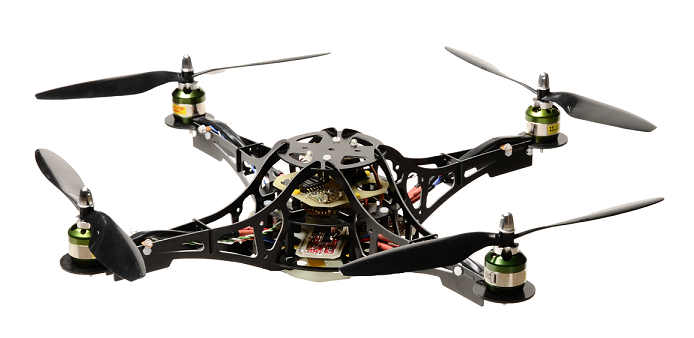
\includegraphics[width=1.00\textwidth]{03_Grafiken/QuadrocopterImage.png}
\end{center}

To achieve horizontal movement, the quadrocopter gets pitched, and by crossover speed up and slowdown of the propellers, it is possible to achieve vertical rotation.
The quadrocopter, this project is based on, gets steered by a four-way remote control. The pilot is able to control the horizontal angles, the vertical rate of rotation and the average speed of the propellers. So the quadrocopter definetely needs an interface, to interpret the commands of the remote control and calculate the engine speed of every motor/propeller. In other words - an embedded controller is needed.
State of the art is a cascaded PI controller, which works fine. Nevertheless it is reasonable to design and implement this mysterious state space controller, to see if it works as well as the PI controller or even better. Besides, a state space controller has some advantages over a classical PID controller.

The development of the controller is an engineering process, that needs structured proceeding, so the next step of this paper is a view on the project management and the structure of this document.

\pagestyle{fancy}
\subsection{V-Model}\label{chapter_V_MODEL}

The project was realized on the basis of the V-Model. The V-Model is a common graphical model to plan an engineering process, that get's customized for each project. In the following, the customized V-Model for this project will be explained.

\begin{figure}[htbp]
	\centering
		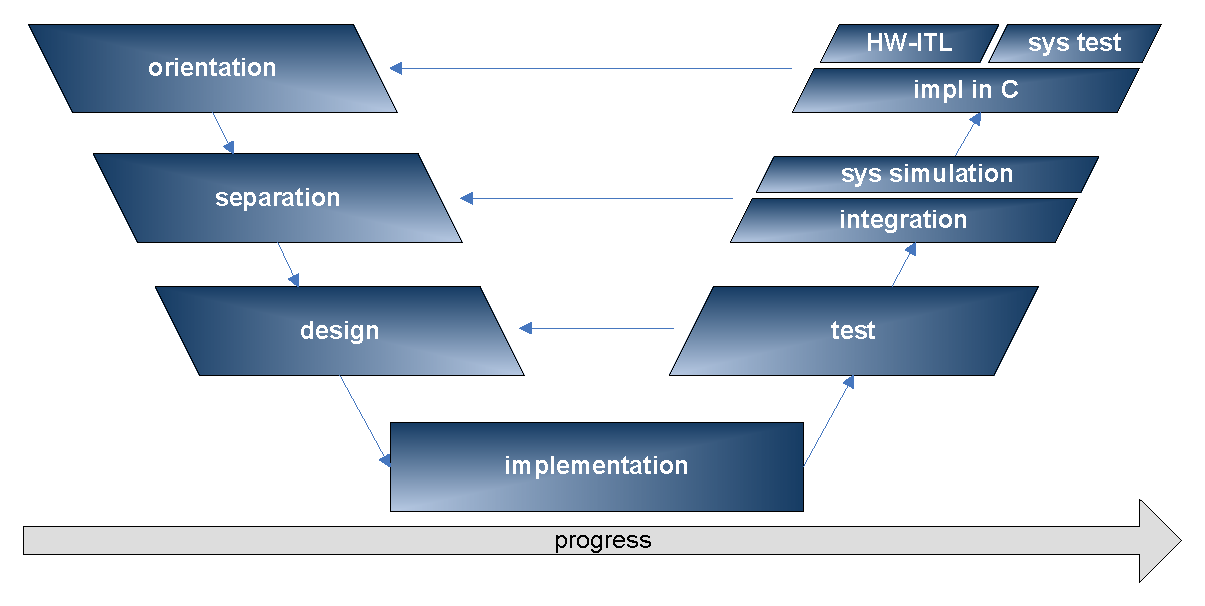
\includegraphics[width=1.00\textwidth]{03_Grafiken/V_Model.pdf}
	\caption{Customized V-Model for this project}
	\label{fig:V_Model}
\end{figure}

Due to a solid basis, on which this project can be build on, the first thing to do is to learn the ropes. The main topic in this step is to understand the quadrocopter's physical model and its already existing model in MATLAB Simulink - and certainly the functionality of a state space controller. An other topic of the orientation-part is to define the requirements. \\
The next step is to separate the relevant part of the Simulink model, so it is possible to work at one 'module', which alleviates to keep the overview. On the basis of this separate part, the next step can be done, which is the beginning of the real project - the design of the state space controller. The lowermost crossbar is the main topic in this engineering process, which means the implementation of the state space controller in MATLAB Simulink. \\
The lowermost part of the right leg of the 'V' includes the test, in this case the simulation, of the implemented state space controller. If there are failures - for example unexpected behavior of a controlled variable, the way follows the lowermost arrow, which guides from the right to the left, back to the design of the state space controller. This circle gets run through, until there are no failures at all. Then the process climbs to the next step, in this case the integration of the state space controller into the original, non-separated Simulink model of the quadrocopter. Then testing, which means still simulation, starts again. If there are failures, the way follows the middle horizontal arrow back to the separation part, because apparently the separated process and the original process don't match. If there are no failures in the system-simulation-part, the next step upward to 'implementation in C' can be done. In this part the graphical model of Simulink gets converted in C-code which is executable by the microcontroller installed in the quadrocopter. This code has to be tested \textbf{H}ardware-\textbf{I}n-the-\textbf{L}oop (HIL) on the real microcontroller. This means, that the code is executed on the real microcontroller, but the output, in this case the actuating variables, gets looped back into the simulation in MATLAB Simulink, which safes ressources, because critical failures can be detected without risking a crash of the quadrocopter. Last but not least, if everything looks great in the HIL simulation, the state space controller gets tested and fine-tuned 'on the fly' with the quadrocopter.

This document leads through this whole engineering process chapter by chapter, starting with understanding the quadrocopter's physical model (chapter \ref{chapter_PHYSICAL_MODEL}) and its model in MATLAB Simulink (chapter \ref{chapter_MATLAB_MODEL}). The next step is to understand the background and layout of a state space controller in chapter \ref{chapter_THEORY}. Then, with this knowledge, the next step is to design and implement the controller in MATLAB/Simulink in chapter \ref{chapter_DESIGN_AND_IMPL} and run simulations in MATLAB Simulink to validate the functionality of the controller in chapter \ref{chapter_TEST}. After that, the implementation of the controller in C is the topic of chapter \ref{chapter_IMPLC}, leading to the HIL tests, just as the tests with the real copter in chapter \ref{chapter_TEST}.
At the end of this document you can find some future prospects in chapter \ref{chapter_FUTUREPROSPECTS}.

With the next chapter this documentation changes over to the engineering process, starting with the physics of the quadrocopter, the first step in the V-Model.
\clearpage %neue Seite erzwingen

\clearpage %neue Seite erzwingen

\pagestyle{fancy}
\section{Physical Model of the quadrocopter}\label{chapter_PHYSICAL_MODEL}

\pagestyle{fancy}
\subsection{Earthframe and bodyframe}\label{chapter_EQUATIONS_OF_MOTION}

This - and the following - chapter discusses the behaviour of a quadrocopter. To achieve a better understanding, graphics with a simplified model of the quadrocopter are used. This model consists of a middle cross, and the four rotors with arrows, showing the direction of rotation. The rotor at the front is marked in yellow.
Placing a coordinate system on the cross of the quadrocopter, the x-axis points to the front, the y-axis to the left and the z-axis points upwards. This coordinate system is called the bodyframe and is shown in red in the picture below.

\begin{figure}[htbp]
	\centering
		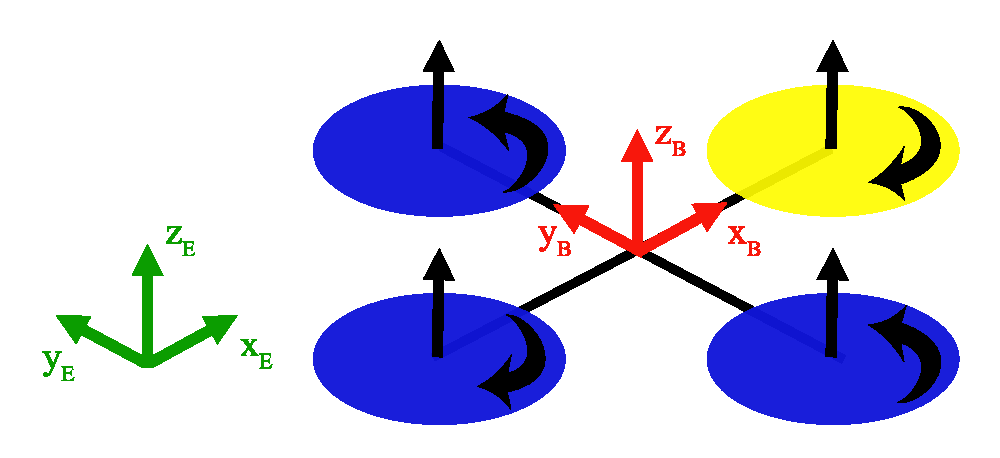
\includegraphics[width=0.7\textwidth]{03_Grafiken/EFrameBFrame.pdf}
	\caption{Earthframe (green) and bodyframe (red)}
	\label{fig:EFrameBFrame}
\end{figure}

The green coordinate system is called the earthframe. This coordinate system is fix and independent of the movement of the quadrocopter. It describes the position of the copter, whereat the copter is interpreted as a point. It also describes the associated velocities and accelerations in direction of x, y and z of the earthframe.
So the earthframe does not contain information about the attitude of the quadrocopter. This information is held by the bodyframe, that includes the angles of the coordinate system in relation to the earthframe, as well as the angular rates and -accelerations. It also holds information about the movement in direction of the axis of the bodyframe coordinate system, wherat the movement in direction of x and y of the bodyframe is a side effect of gravity, while movement in direction of z can be controlled directly.

So, 'sitting' on the bodyframe of the quadrocopter, it is not possible to know the position in space, but it is possible to know the deviation from horizontal in degrees as well as the vertical speed of spinning. Sitting on the eartframe, it is possible to see where the quadrocopter is, and how fast it is moving, but it is impossible to know if it is perhaps flying upside down.

Though these two frames hold different information, there is a mathematical association in between. This is explained in a simple two-dimensional example below.

\begin{figure}[htbp]
	\centering
		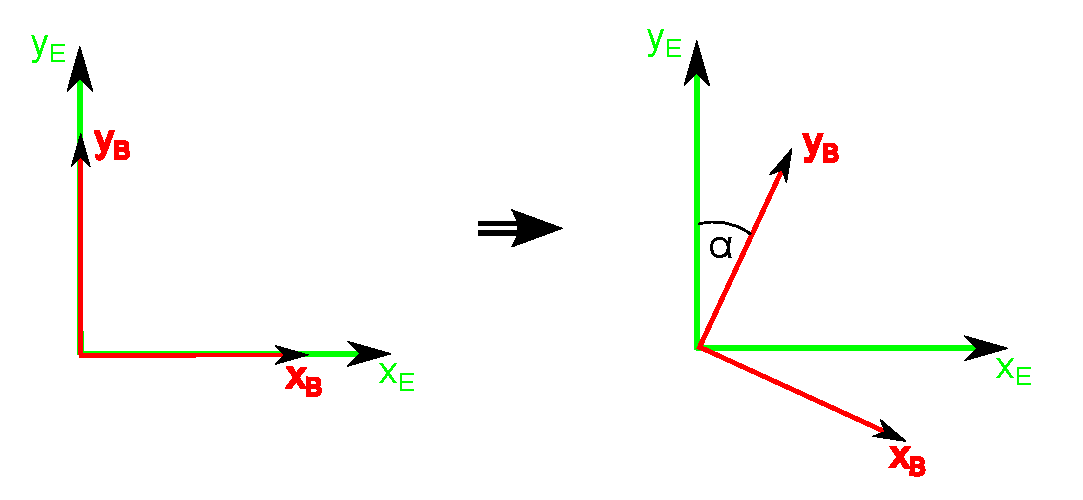
\includegraphics[width=1.0\textwidth]{03_Grafiken/2DFrames.pdf}
	\caption{Association between earthframe and bodyframe}
	\label{fig:2DFrames}
\end{figure}

In the left picture, the two-dimensional bodyframe is congruent with the earthframe. If there is a constant velocity $v_{yB}$ in direction of $y_B$:
\begin{center}
	$v_{yE} = v_{yB}$
\end{center}
Furthermore 
\begin{center}
	$v_{xE} = 0$ 
\end{center}
In the second picture, the bodyframe is rotated a constant angle alpha; $v_{yB}$ is still constant. Now it is: 
\begin{center}
$v_{yE} = cos(\alpha)*v_{yB}$
\end{center}
and 
\begin{center}
$v_{xE} = sin(\alpha)*v_{yB}$
\end{center}
So it is possible to transform coordinates of the bodyframe into coordinates of the earthframe and vice versa. %Earthframe, Bodyframe
\clearpage %neue Seite erzwingen

\pagestyle{fancy}
\subsection{Motion of the quadrocopter}\label{chapter_BASICS}

Theoretically a quadrocopter has six degrees of freedom: 
\begin{enumerate}
		\item Moving in direction of x (forward, backward)
		\item Moving in direction of y (left, right)
		\item Moving in direction of z (up, down)
		\item Rotation around the x-axis, called 'Roll'
		\item Rotation around the y-axis, called 'Pitch'
		\item Rotation around the z-axis, called 'Yaw'
\end{enumerate}
Effectively there are only four degrees of freedom, because movement in direction of x and y is only a side-effect by gravity, like it is described in chapter \ref{chapter_EQUATIONS_OF_MOTION}. 
These four degrees of freedom are exemplified in the following.

\subsubsection{Thrust}
\begin{figure}[htbp]
	\centering
		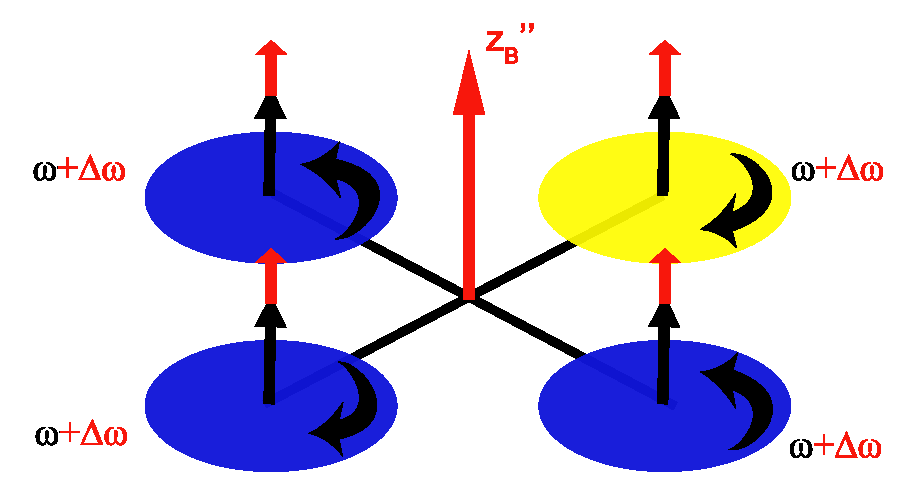
\includegraphics[width=0.7\textwidth]{03_Grafiken/Thrust.pdf}
	\caption{Thrust}
	\label{fig:Thrust}
\end{figure}

If all rotors are spinning with constant angular rate $\omega$ and a new offset $\Delta\omega$ is added, the ascending force of each rotor increases in same way, which results in a force vector, pointing in direction of z of the bodyframe. So the quadrocopter accelerates in direction of z.

\subsubsection{Pitch}
\begin{figure}[H]
	\centering
		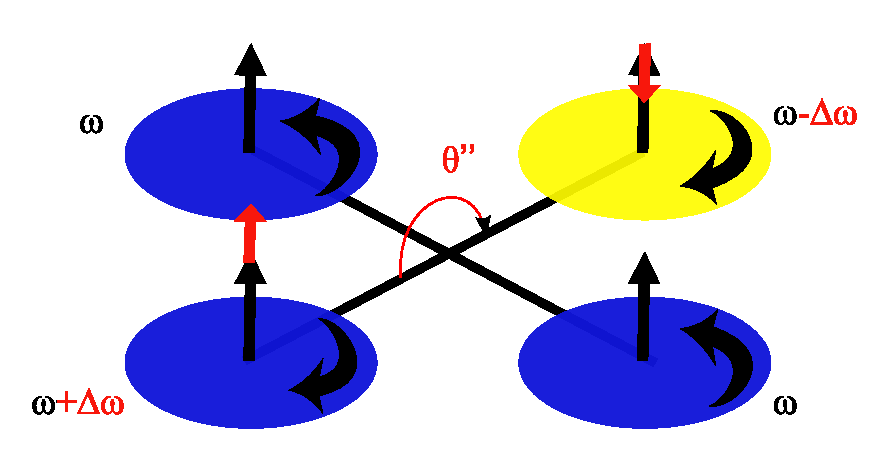
\includegraphics[width=0.7\textwidth]{03_Grafiken/Theta.pdf}
	\caption{Pitch}
	\label{fig:Theta}
\end{figure}
To achieve forward-pitching, the rotor in front is slowed down, what means a negative offset $\Delta\omega$. In addition a positive offset is added to the rear motor. The result is a change of the angular acceleration and therefore a change of the angle $\theta$ (theta).

\subsubsection{Roll}
\begin{figure}[htbp]
	\centering
		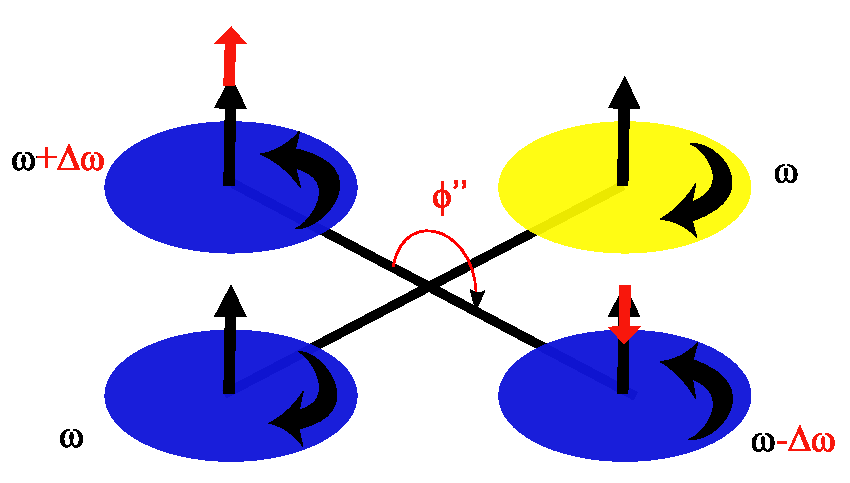
\includegraphics[width=0.7\textwidth]{03_Grafiken/Phi.pdf}
	\caption{Roll}
	\label{fig:Phi}
\end{figure}
The principle to get a roll movement is the same one, like it is used for the pitch movement. To achieve a roll movement to the right, a negative offset $\Delta\omega$ is added to the rotor on the right side of the quadrocopter. In addition a positive offset is added to the left rotor. Again the result is a change of the angular acceleration and therefore a change of the angle $\Phi$(phi)

\subsubsection{Yaw}
\begin{figure}[htbp]
	\centering
		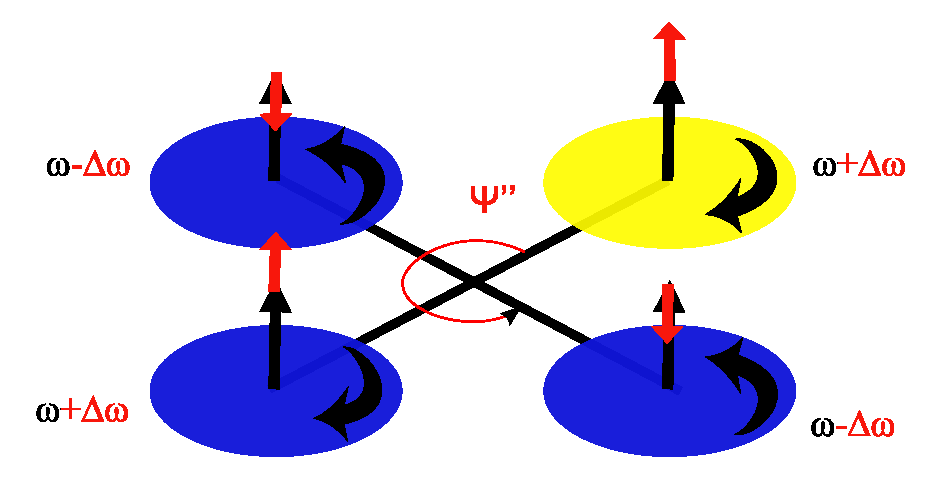
\includegraphics[width=0.7\textwidth]{03_Grafiken/Psi.pdf}
	\caption{Yaw}
	\label{fig:Psi}
\end{figure}
To achieve rotation around the z-axis, called 'yaw' is more tricky than the roll and pitch movements.
It is visible in the grapics, that the rotors at the front and the back of the quadrocopter spin clockwise, while the two rotors on the side of the quadrocopter spin counterclockwise. This is necessary because of the inertia of the propellers. If all propellers would spin clockwise, the quadrocopter would steadily rotate counterclockwise. This effect is used, to rotate the quadrocopter.
To achieve a rotation counterclockwise, a positive offset is added to the front rotor and the rear rotor. To intensify this effect and avoid thrust, the left and the right rotor, which hold up, are slowed down by adding a negative offset to their motor speed. The result is a vertical, counterclockwise rotation $\Psi$(psi). %Winkel, Geschwindigkeiten, Beschleunigungen
\clearpage %neue Seite erzwingen

\pagestyle{fancy}
\subsection{Process variables}\label{chapter_VARIABLES}
This chapter gives a short overview over the controlled process variables, the actuating variables and the set points. The grafic below shows, where these values are placed in the closed loop. \\
The first rectangle represents the controller, that is designed and implemented in this project. The second rectangle represents the quadrocopter; the process that has to be controlled.
\begin{figure}[H]
	\centering
		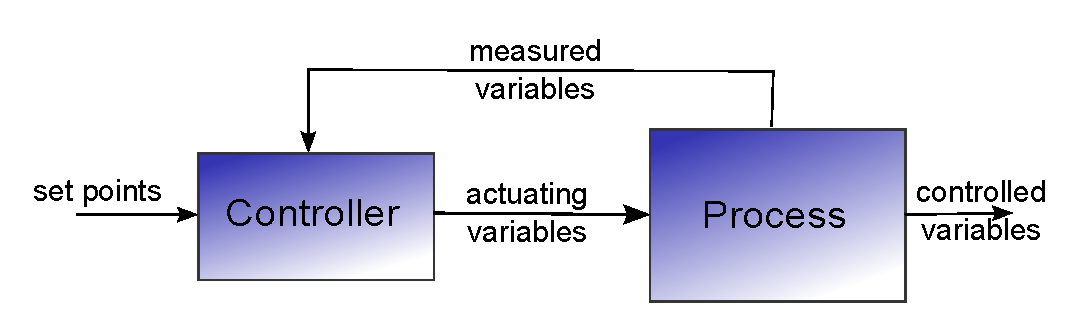
\includegraphics[width=0.9\textwidth]{03_Grafiken/closed_loop_abstract.pdf}
	\caption{closed loop abstract}
	\label{fig:closed loop abstract}
\end{figure}
The set points are equal to the controlled variables. The pilot is able to control the \textit{angle of phi} (roll), the \textit{angle of theta} (pitch) and the \textit{rate of psi} (yaw). In chapter \ref{chapter_BASICS}, one degree of freedom is \textit{thrust}, which in some way also is a set point, but it is not a controlled variable, but directly controlled by the pilot. Actually it is an offset, that is added to the actuating variables, that have been calculated by the controller before.
These actuating variables are some sort of normalized forces, every propeller has to provide. They are called 'pseudo forces' in this document. \\
Last but not least, there are the measured variables, that are needed by the controller. These variables are content of the next chapter.	%Regel und Stellgr��en
\clearpage %neue Seite erzwingen
\subsection{Sensors}\label{chapter_SENSORS}
Without sensors it is not possible to control any process. The quadrocopter carries two sensors:
\begin{enumerate}
	\item A gyro-sensor, that provides angular rates in direction of \textit{phi}(roll), \textit{theta}(pitch) and \textit{psi}(yaw) of the bodyframe. 
	\item A linear-acceleration-sensor, that provides accelerations in direction of \textit{x}, \textit{y} and \textit{z} of the bodyframe.
\end{enumerate}
The measured variables of the first sensor are used directly by the controller. The variables of the second sensor - the linear-acceleration-sensor - are used to calculate the real angles \textit{phi} and \textit{theta}. The angle of \textit{psi} is not relevant for the controller, so the \textit{z}-value of the sensor is not relevant as well.	%Gemessene Gr��en
\clearpage %neue Seite erzwingen

\clearpage %neue Seite erzwingen

\pagestyle{fancy}
\section{Model of the quadrocopter using MATLAB Simulink}\label{chapter_MATLAB_MODEL}

The topic of this chapter is the graphical model of the quadrocopter in MATLAB Simulink.
Actually it describes the whole control loop, including the controller and the sensors, called closed loop. While the first subchapter shows an overview over the complete loop, each part of the loop is discussed separately in the following subchapters.

\pagestyle{fancy}
\subsection{Overview}\label{chapter_OVERVIEW}
This chapter leads once through the control loop, that is pictured below.
\begin{figure}[H]
	\centering
		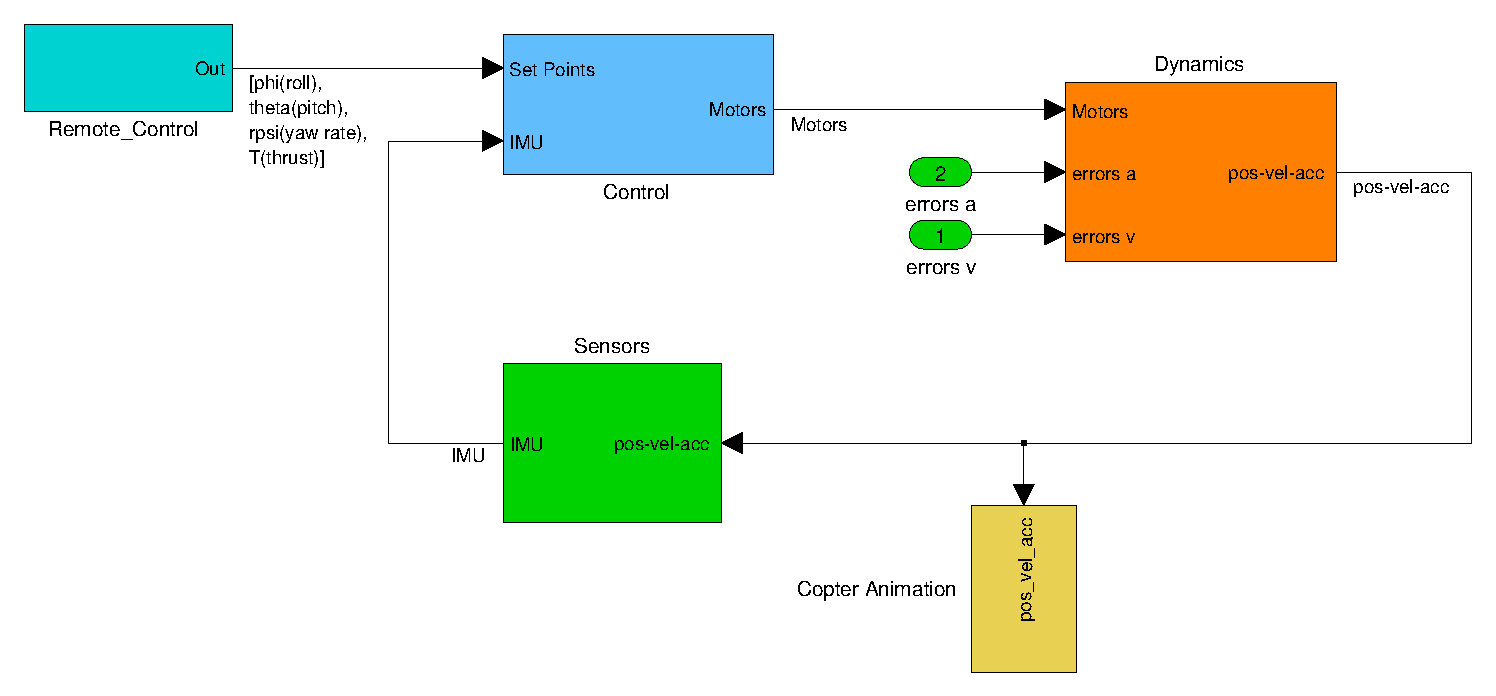
\includegraphics[width=1.0\textwidth]{03_Grafiken/MATLAB_Overview.pdf}
	\caption{Overview Closed Loop}
	\label{fig:MATLAB Overview}
\end{figure}
The cyan-colored block top left, represents the remote control. This block 'generates' the set points. These set points are combined in one vector, consisting of:
\begin{enumerate}
	\item the angle of \textit{phi} (roll)
	\item the angle of \textit{theta} (pitch)
	\item the angular rate of \textit{psi} (yaw rate)
	\item the average motorspeed (thrust)
\end{enumerate}
The next block, colored blue, is the controller block. The state space controller, developed in this project, gets implemented in this block. In there, the set points, given by the first block, get 'converted' into actuating variables. Again, these variables are combined in one vector, consisting of the four pseudo forces.\\
This vector is connected to the input of the next (orange) block, that represents the quadrocopter. Symbolic blocks represent the physical characteristics of the copter. So this block calculates, how the speed of each motor affects the movement of the copter. The result is a big vector called 'pos-vel-acc', which stands for 'positions-velocities-accelerations'. So this vector consists of all states of the quadrocopter, meaning the actual angle of \textit{phi}, \textit{theta}, \textit{psi}; its angular \textit{rate of phi}, \textit{theta}, \textit{psi}; its actual position in \textit{x}, \textit{y}, \textit{z} of the earthframe, and so on. The complete vector is pictured in chapter \ref {chapter_DYNAMICS_BLOCK}.
This vector is the input of the next block of the closed loop - the sensors block, pictured in green - which returns the measured variables, combined in the vector 'IMU' (Inertial Measurement Unit). This vector consists of:
\begin{enumerate}
	\item acceleration in direction of \textit{x} of the bodyframe
	\item acceleration in direction of \textit{y} of the bodyframe
	\item the angular \textit{rate of phi} (roll rate)
	\item the angular \textit{rate of theta} (pitch rate)
	\item the angular \textit{rate of psi} (yaw rate)
\end{enumerate}
Also connected to the vector 'pos-vel-acc' is the yellow block at the bottom of the model. This block includes the animation of the quadrocopter. Though, this is not a real part of the control loop, it is an important assistance for testing the controller, because it allows to fly the quadrocopter virtually.

The next subchapters will walk once through this whole process, described above, starting with the remote control block.
\clearpage %neue Seite erzwingen

\pagestyle{fancy}
\subsection{Remote control block}\label{chapter_REMOTE_CONTROL_BLOCK}
This chapter will show the 'innards' of the first block, pictured in cyan in Figure \ref{fig:MATLAB Overview}.
\begin{figure}[H]
	\centering
		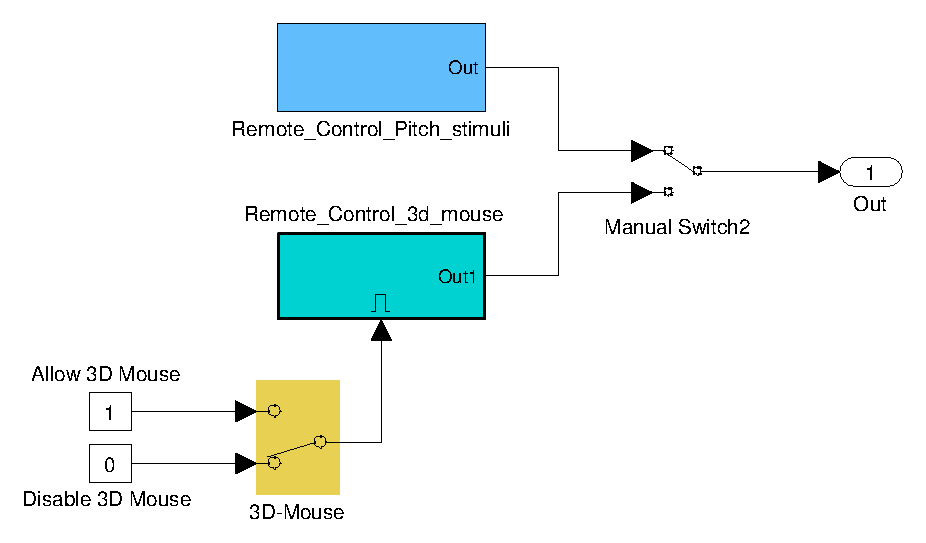
\includegraphics[width=0.8\textwidth]{03_Grafiken/MATLAB_Remote_Control_Overview.pdf}
	\caption{Remote control block overview}
	\label{fig:Remote control block}
\end{figure}
The cyan block in this figure, allows to connect a 3D-mouse to the computer to steer the quadrocopter in the animation. This research paper doesn't elaborate on this block.
The block in light-blue allows to generate manual stimuli. The content of this block is showed below.
\begin{figure}[htbp]
	\begin{minipage}[t]{6cm}
		\vspace{0pt}
		\centering
		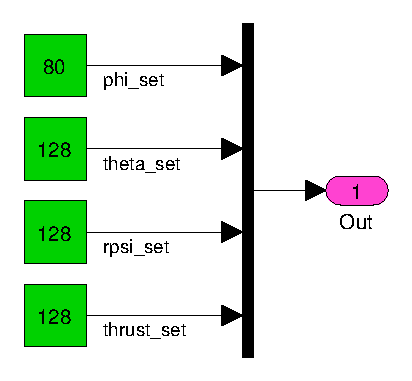
\includegraphics[width=6cm]{03_Grafiken/MATLAB_Remote_Control_Stimuli.pdf}
		\caption{Stimuli}
		\label{fig:Remote control stimuli}
	\end{minipage}
	\hfill
	\begin{minipage}[t]{8cm}
		\vspace{0pt}
		\medskip
		\begin{onehalfspace}
		By double clicking the green blocks, it is possible to change the values of these blocks. The values range 		 
		from 0 to 255, where 128 means angle zero for phi (roll) and theta (pitch) or rather angular rate zero for 			rate of psi (yaw rate). Value 255 of thrust means 				
		full-speed to all motors.
		So the stimuli in the left figure say 'no pitching, no yaw rate and a negative angle towards the horizontal 	
		(roll left) at half thrust'.
		\end{onehalfspace}
	\end{minipage}
\end{figure}
\clearpage %neue Seite erzwingen

\pagestyle{fancy}
\subsection{Controller block}\label{chapter_CONTROLLER_BLOCK}
The figure below shows the content of the light blue 'Control' block in figure \ref{fig:MATLAB Overview}.
\begin{figure}[H]
	\centering
		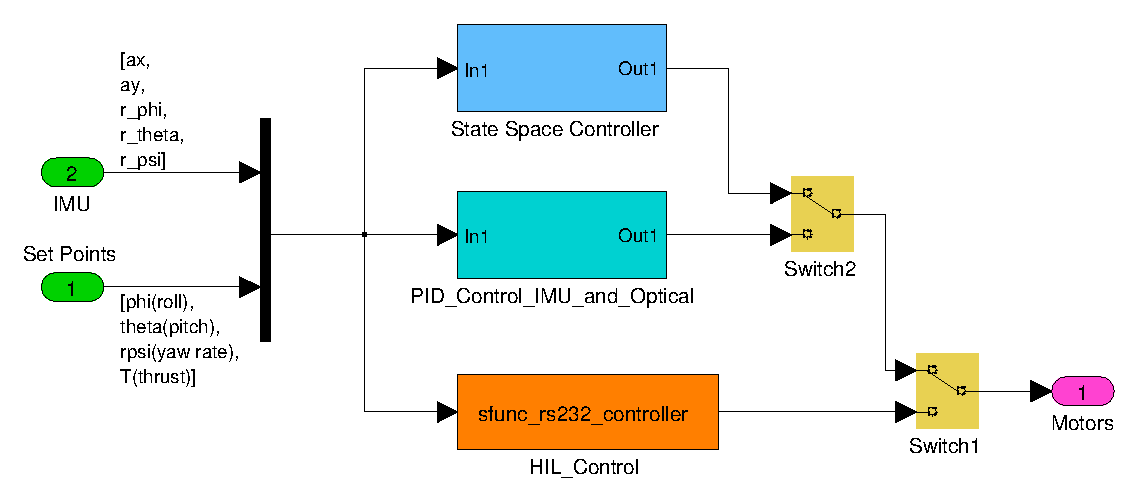
\includegraphics[width=1.0\textwidth]{03_Grafiken/MATLAB_Controller.pdf}
	\caption{Controller block}
	\label{fig:Controller block}
\end{figure}
The controller block has two inputs, 'Set Points' and sensor values ('IMU'). The black bar combines them to one vector with the elements:
\begin{enumerate*}
	\item \textit{ax} (acceleration in direction of x of bodyframe; IMU)
	\item \textit{ay} (acceleration in direction of y of bodyframe; IMU)
	\item \textit{rphi} (rate of phi; IMU)
	\item \textit{rtheta} (rate of theta; IMU)
	\item \textit{rpsi} (rate of psi; IMU)
	\item \textit{phi} (Set point of phi)
	\item \textit{theta} (Set point of theta)
	\item \textit{rpsi} (Set point or rate of psi)
	\item \textit{thrust} (Set point of thrust)
\end{enumerate*}
This vector is the input of three blocks. The topmost, light blue block is the new state space controller, implemented in this project. The second block, pictured in cyan, is the, already existing, PID-controller. The lowermost, orange block is the block, that is used to test the quadrocopter hardware in the loop (HIL).
The two switches on the right side define, which controller is enabled or rather whose actuating variables are connected to the process. The output of each controller block are the 'pseudo forces', every propeller has to provide.
\clearpage %neue Seite erzwingen

\pagestyle{fancy}
\subsection{Dynamics block}\label{chapter_DYNAMICS_BLOCK}
The MATLAB Simulink block, that includes the physical model of the quadrocopter, pictured in orange in figure \ref{fig:MATLAB Overview}, is the topic of this chapter.
As this model doesn't fit on one page, it is split up into multiple sections. The picture below shows the whole process, divided into four areas. The following chapters discuss these areas as appropriate. It is not necessary to discuss each block in detail, to be able to develop a controller for this process.
\begin{figure}[H]
	\centering
		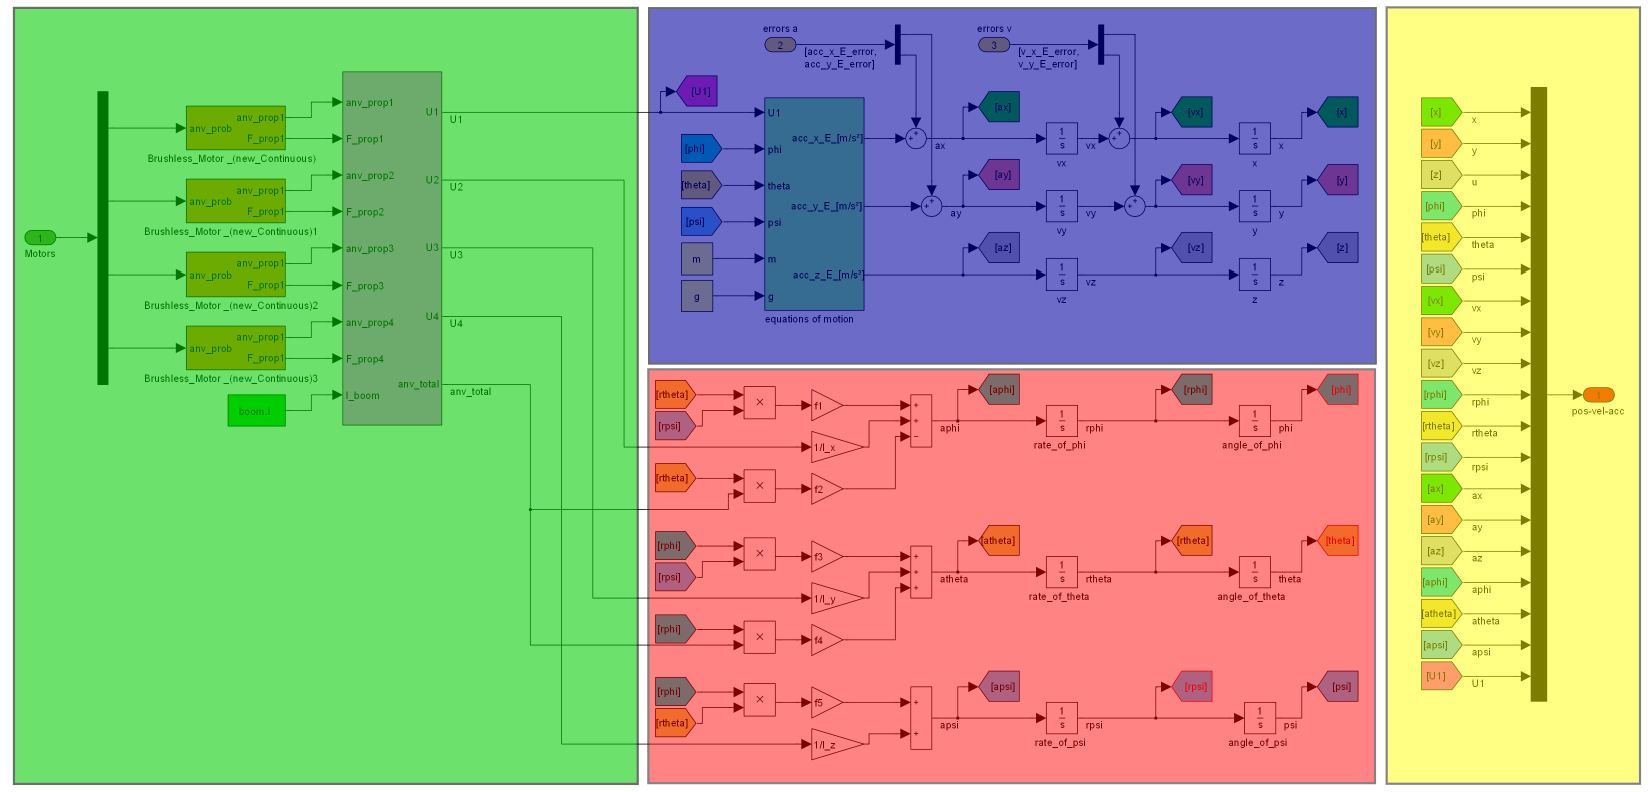
\includegraphics[width=1.0\textwidth]{03_Grafiken/MATLAB_Dynamics_Sections.pdf}
	\caption{Sections of the Dynamics block}
	\label{fig:MATLAB Dynamics Sections}
\end{figure}
\clearpage %neue Seite erzwingen

\subsubsection{Dynamics of the four motors (green section)}\label{chapter_GREEN_SECTION}
The green section has one input vector. It holds the pseudo forces, every propeller has to provide, given by the controller.
\begin{figure}[H]
	\centering
		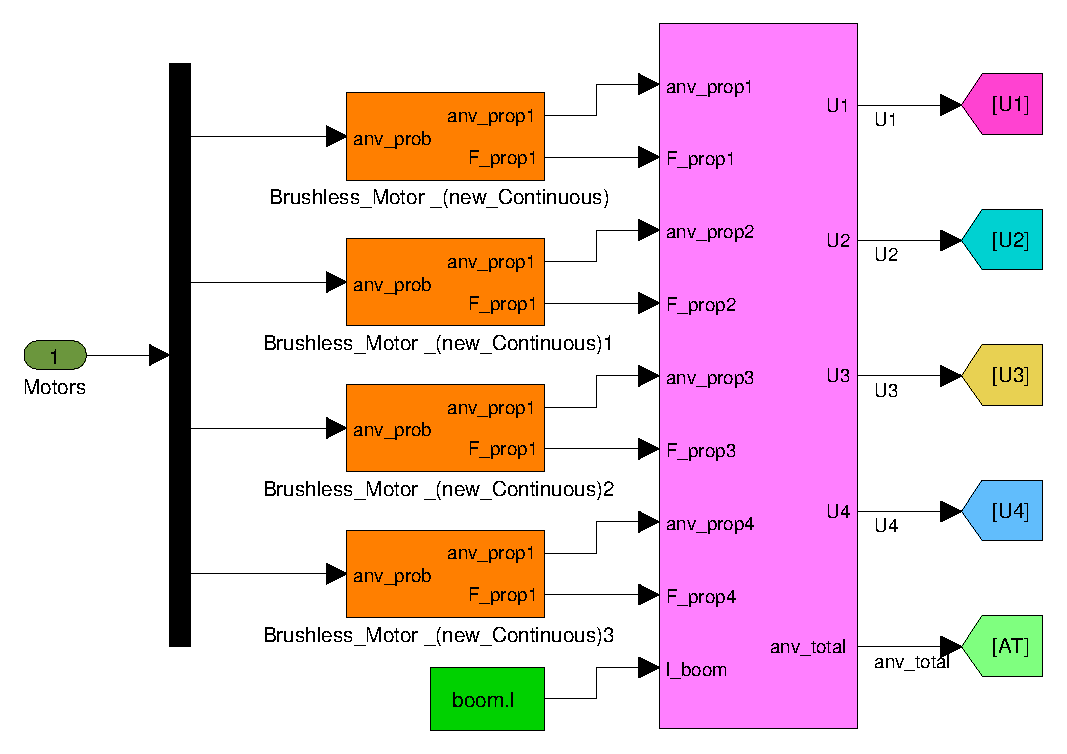
\includegraphics[width=0.8\textwidth]{03_Grafiken/MATLAB_Dynamics1.pdf}
	\caption{Green section}
	\label{fig:MATLAB Dynamics1}
\end{figure}
Each pseudo force is the input of one motor (orange blocks). 
Double clicking on one of the motors opens the graphic below.
\begin{figure}[H]
	\centering
		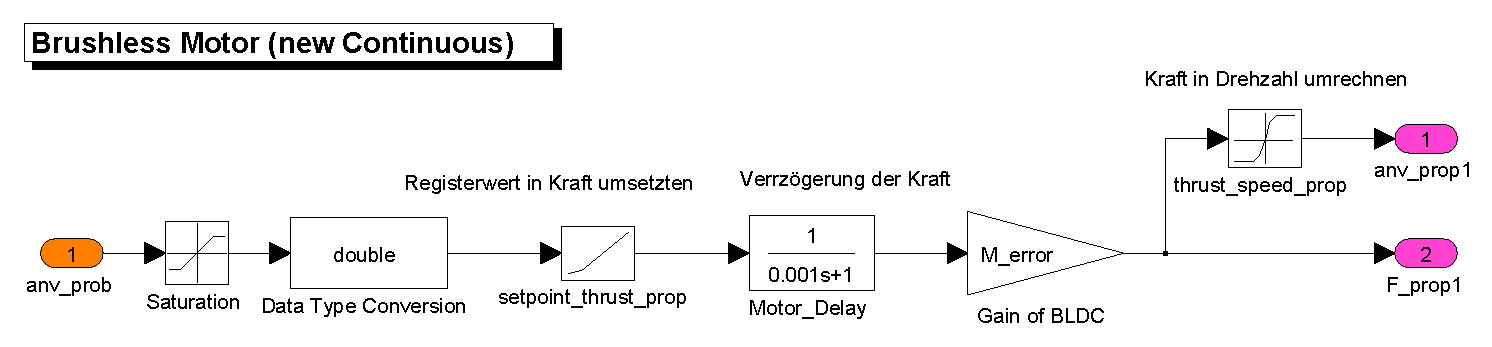
\includegraphics[width=1.0\textwidth]{03_Grafiken/motorWithDelay.pdf}
	\caption{Motor}
	\label{fig:motor}
\end{figure}
The pseudo force, coming from the controller, gets converted into a real force by the characteristic diagram 'setpoint\_thrust\_prop'. Due to the inertia of the propeller this force is delayed by a PT1-element.
The motor has two outputs, \textit{anv\_propX} and \textit{F\_propX}, where \textit{F\_prop} is the force, the propeller produces vertically to itself. \textit{anv\_prop} is the angular velocity of the propeller, that gets calculated by the characteristic diagram 'thrust\_speed\_prop'.

The big purple block in figure \ref {fig:MATLAB Dynamics1} uses these forces to calculate the angular accelerations in direction of phi (U2), theta(U3) and psi(U4). For this calculation the lever principle (force * lever) is used. The small green block \textit{boom.l} provides the information about the levers. 
The purple block also has two other output values \textit{U1} and \textit{AT}. \textit{U1} is the sum of all propeller forces \textit{F\_propX}, \textit{AT} is the sum of all rotary speeds \textit{anv\_propX}.

\subsubsection{Dynamics of quadrocopter in bodyframe (red section)}\label{chapter_RED_SECTION}
This section represents the bodyframe of the quadrocopter and consits of three very similar lines.
\begin{figure}[H]
	\centering
		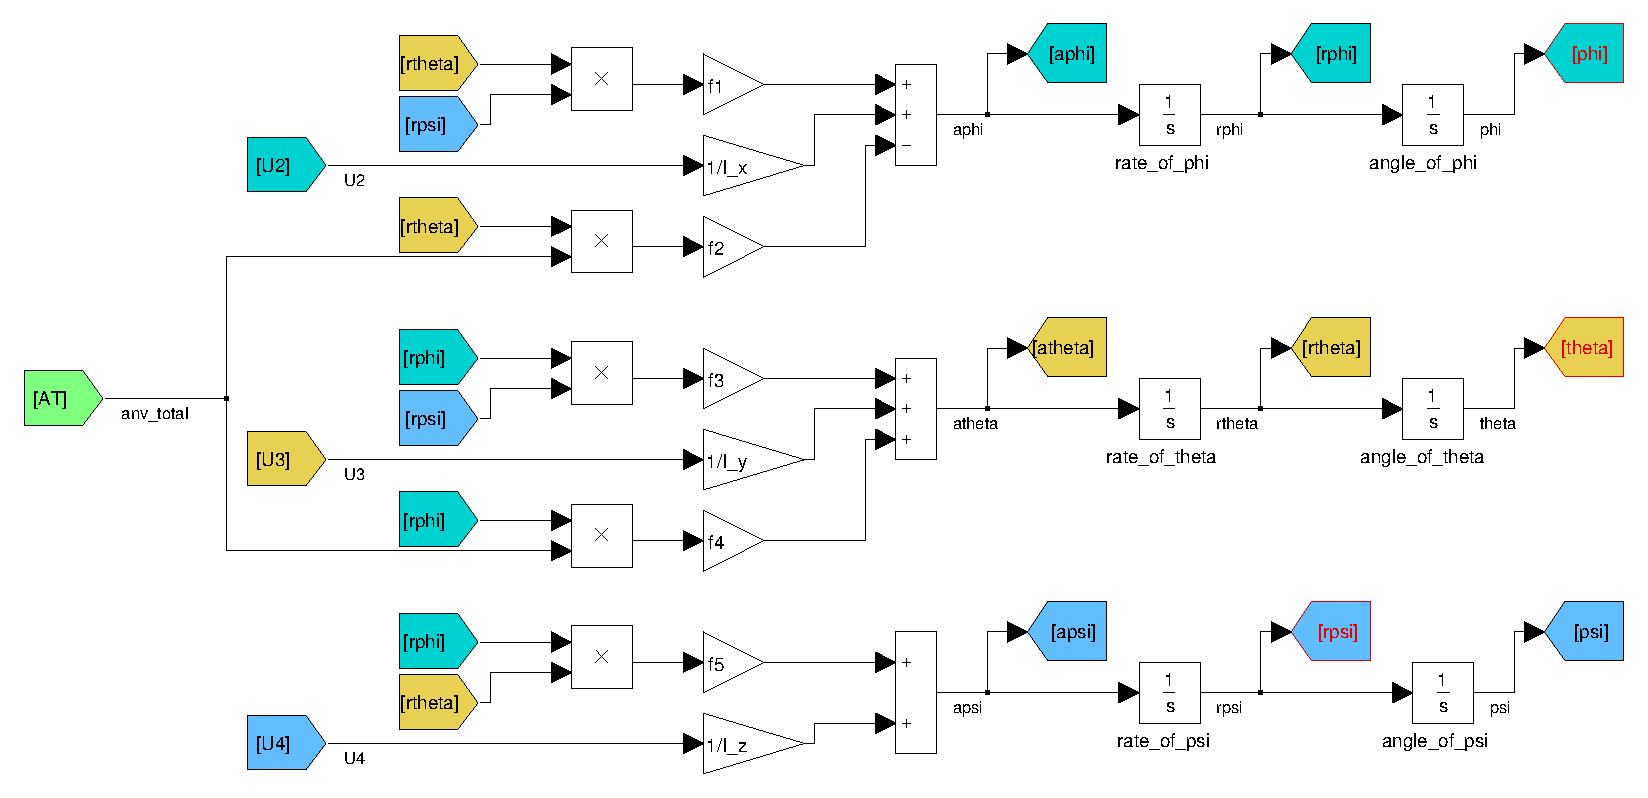
\includegraphics[width=1.0\textwidth]{03_Grafiken/MATLAB_Dynamics2.pdf}
	\caption{Red section}
	\label{fig:MATLAB Dynamics2}
\end{figure}
The topmost line uses the rate of theta \textit{rtheta}, the rate of psi \textit{rpsi}, the angular acceleration in direction of phi \textit{U2} and the sum of all rotary speeds \textit{AT} to calculate the resulting angular acceleration in direction of phi (\textit{aphi}) of the physical model. This shows, that movement in direction of \textit{phi} is influenced by movement in direction of \textit{theta} and \textit{psi}. This is momentous for the development of the controller.\\
The angular acceleration gets integrated once, resulting in the angular rate of phi \textit{rphi}, and twice, resulting in the angle \textit{phi}. The other two lines for \textit{theta} and \textit{psi} are very similar, so this is not discussed here in detail. The controlled variables \textit{phi}, \textit{theta} and \textit{rpsi} are pictured in red letters.
 
\subsubsection{Dynamics of quadrocopter in earthframe (blue section)}\label{chapter_BLUE_SECTION}
While the red section represents the bodyframe, this section represents the earthframe.
\begin{figure}[H]
	\centering
		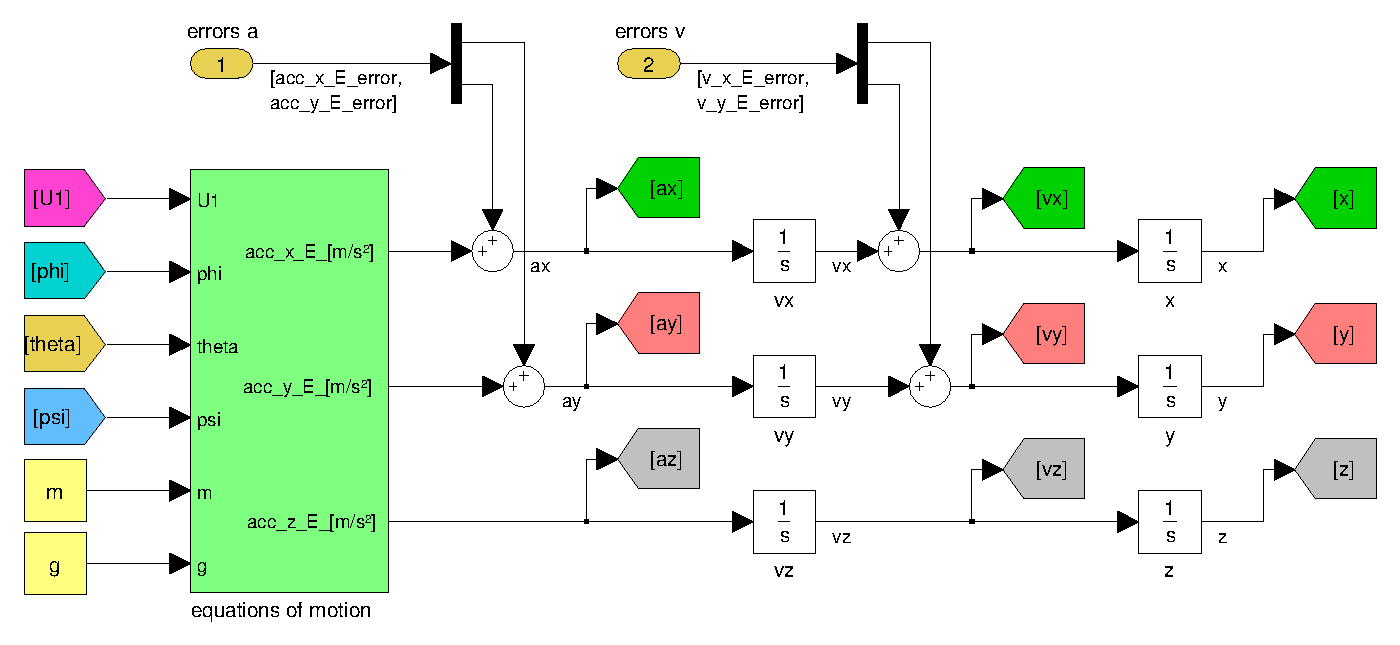
\includegraphics[width=1.0\textwidth]{03_Grafiken/MATLAB_Dynamics3.pdf}
	\caption{Blue section}
	\label{fig:MATLAB Dynamics3}
\end{figure}
At the 'input' of this section is one big, non-linear block, 'equations of motion'. It uses the 'output' of the red section, \textit{phi}, \textit{theta} and \textit{psi}, the sum of all propeller forces \textit{U1} and two constants m (mass of the quadrocopter) and g (gravitational acceleration) to calculate the accelerations in direction of x, y and z of the earthframe. These values get integrated to gain the linar speeds and the position of the quadrocopter. By using the inputs 'error a' and 'error v', it is possible to simulate wind.
\clearpage %neue Seite erzwingen

\subsubsection{Combination of all signals (yellow section)}\label{chapter_YELLOW_SECTION}
The yellow section shows the output vector of the dynamics block, called \textit{pos\_vel\_acc} (positions-velocities-accelerations).
\begin{figure}[htbp]
	\begin{minipage}[t]{8cm}
		\vspace{0pt}
		\begin{singlespace}
			\medskip
			\medskip
			\medskip
			\begin{itemize}
			\item position \textit{x} of earthframe
			\item position \textit{y} of earthframe
			\item position \textit{z} of earthframe
			\item angle \textit{phi} of bodyframe
			\item angle \textit{theta} of bodyframe
			\item angle \textit{psi} of bodyframe
			\item linear speed in direction of \textit{x}
			\item linear speed in direction of \textit{y}
			\item linear speed in direction of \textit{z}
			\item angular speed in direction of \textit{phi}
			\item angular speed in direction of \textit{theta}
			\item angular speed in direction of \textit{psi}
			\item linear acceleration in dir. of \textit{x}
			\item linear acceleration in dir. of \textit{y}
			\item linear acceleration in dir. of \textit{z}
			\item angular acceleration in dir. of \textit{phi}
			\item angular acceleration in dir. of \textit{theta}
			\item angular acceleration in dir. of \textit{psi}
			\item sum of all propeller forces
			\end{itemize}
		\end{singlespace}
	\end{minipage}
	\hfill
	\begin{minipage}[t]{6.5cm}
		\vspace{0pt}
		\centering
		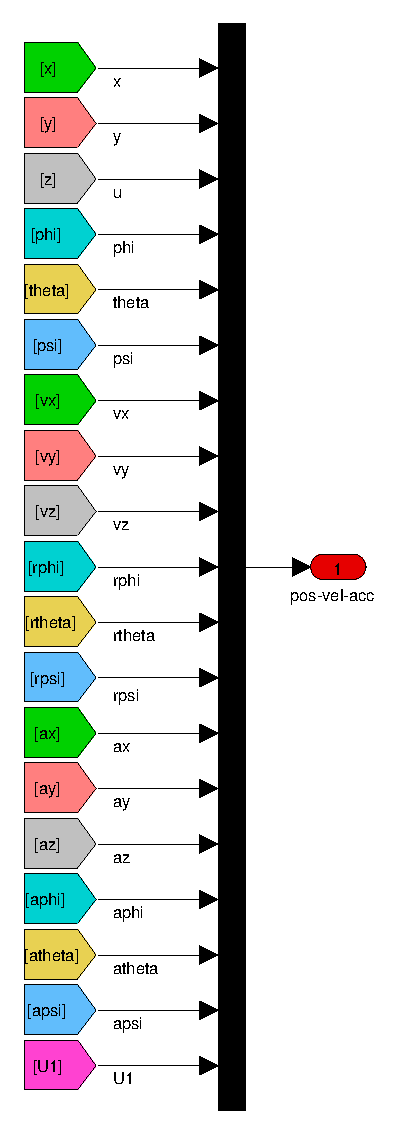
\includegraphics[width=6.15cm]{03_Grafiken/MATLAB_Dynamics4.pdf}
		\caption{Yellow Section}
		\label{fig:MATLAB Dynamics4}
	\end{minipage}
\end{figure}
\clearpage %neue Seite erzwingen

\pagestyle{fancy}
\subsection{Sensors block}\label{chapter_SENSORS_BLOCK}
The first important hint in this chapter is, that the input is on the right side of the model, because the sensors are in the backward line of the closed loop in figure \ref{fig:MATLAB Overview} (green block).
\begin{figure}[H]
	\centering
		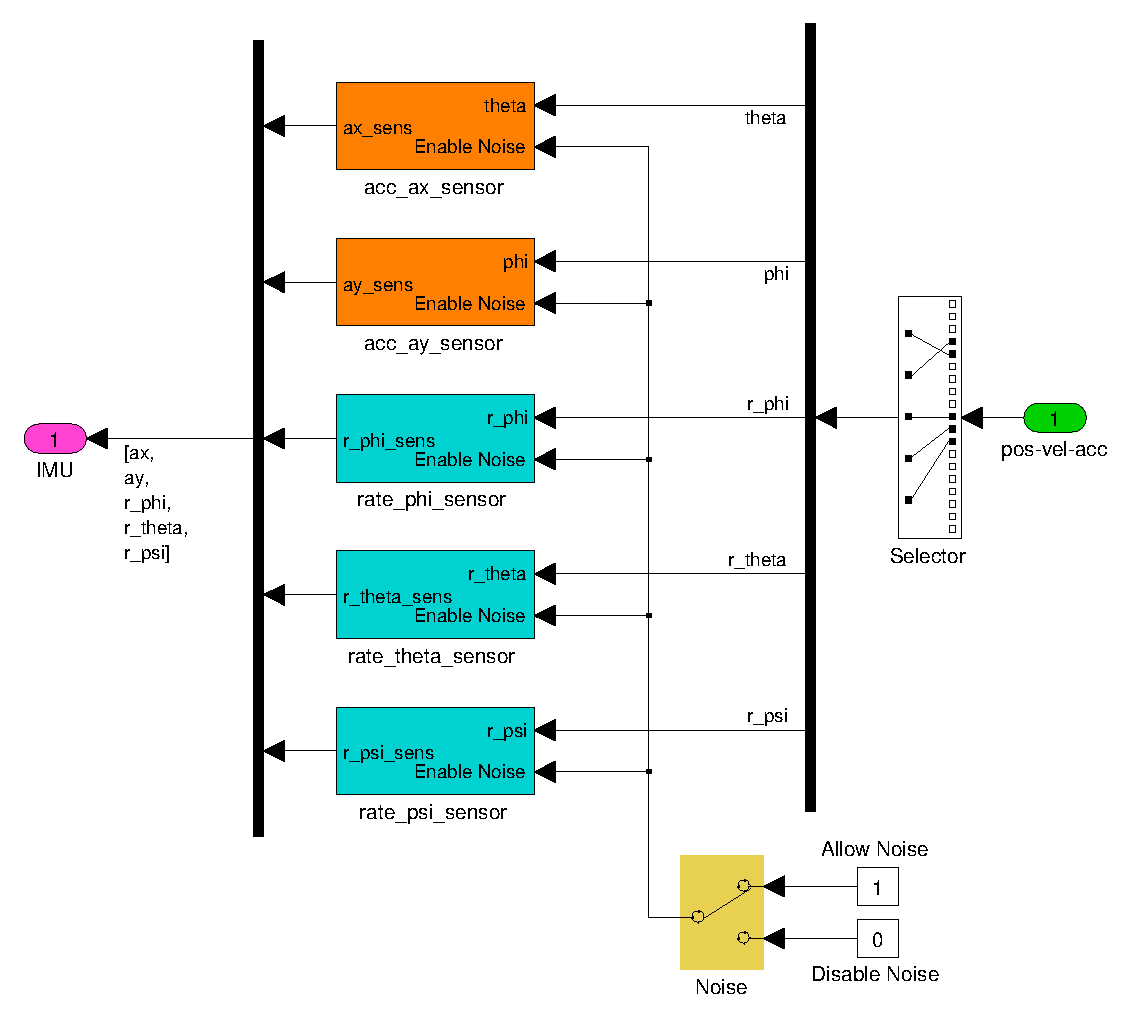
\includegraphics[width=0.9\textwidth]{03_Grafiken/MATLAB_Sensors.pdf}
	\caption{Sensors block}
	\label{fig:Sensors block}
\end{figure}
The first block after the input is a line-selector, that picks the elements out of the \textit{pos\_vel\_acc}-vector, that get measured in the real copter by the sensors. These values are the inputs of each sensor. The upper, orange blocks represent the linear acceleration sensors, that measure the accelerations in direction of \textit{x} and \textit{y} of the bodyframe. These accelerations are not contained in the \textit{pos\_vel\_acc}-vector. So, they have to be calculated in the (model of the) sensor, using the angle and a trigonometric function.
The angular velocities are included in the output vector of the dynamics block, so they get directly 'measured' by the sensors. All measured values are combined in the output vector \textit{IMU} of the sensors block. 
\clearpage %neue Seite erzwingen



\clearpage %neue Seite erzwingen

\pagestyle{fancy}
\section{Theory of the state space controller}\label{chapter_THEORY}

\pagestyle{fancy}
\subsection{State space}\label{chapter_StateSpace}

In this section, the basic knowledge for understanding the so-called state space representation, is described. The state space representation is a mathematical system of a physical model. It consists of inputs and outputs and the state variables that are related to the differential equations of that model. One huge advantage of this idea is, that the Laplace transformation is not needed. Therefore the state space representation is also called 'time-domain approach'. Another opportunity is the usage of initial conditions and that a system can have nonlinear constraints. 

So the next step is to understand the state variables. As already mentioned, every state space system consists of inputs, outputs and state variables. These state variables describe the entire state of the system at any time. The simplest way to decide where to set the state variables, is to put them behind every single integrator block. So the state variable itself is behind this block and the corresponding derivative in front. \myfigref{fig:simpleProcess} shows a simple example for a third order system. This system is called a SISO system, that means 'Single Input Single Output'. In this case \textit{u} is the single input and \textit{y} the single output of the system. Besides, there are MIMO systems having 'Multiple Input Multiple Output'. Chapter \ref{chapter_MIMO} handles them.

\begin{figure}
	\centering
		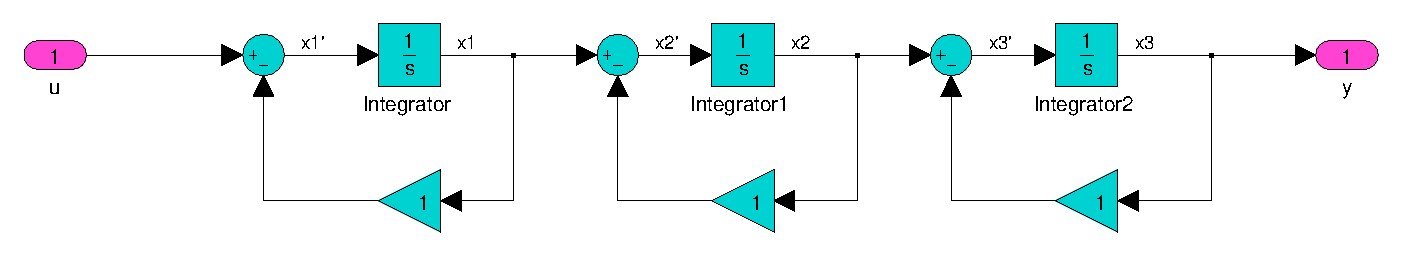
\includegraphics[width=1.00\textwidth]{03_Grafiken/simpleProcess.pdf}
	\caption{Simple example of a SISO process}
	\label{fig:simpleProcess}
\end{figure}

The differential equations for this system look like that:
\begin{align*}
	x1' & = -x1 + u\\ 
	x2' & = x1 - x2\\
	x3' & = x2 - x3\\
	y   & = x3
\end{align*}

These differential equations can be transformed into four matrices:
\begin{align}
\bordermatrix[{[]}]{
    & x1 & x2 & x3 & u \cr
x1' & \colorbox{yellow}{-1} & \colorbox{yellow}{0}  & \colorbox{yellow}{0}  & \colorbox{red}{1} \cr
x2' & \colorbox{yellow}{1}  & \colorbox{yellow}{-1} & \colorbox{yellow}{0}  & \colorbox{red}{0} \cr
x3' & \colorbox{yellow}{0}  & \colorbox{yellow}{1}  & \colorbox{yellow}{-1} & \colorbox{red}{0} \cr
y   & \colorbox{green}{0}   & \colorbox{green}{0}   & \colorbox{green}{1}   & \colorbox{cyan}{0}
}
\end{align}

The most important is the \colorbox{yellow}{A matrix}, called the 'state matrix'. This matrix declares the dependency between all state variables in the whole system. With this matrix it is possible to get information about the response characteristics and the stability of the system. The \colorbox{red}{B matrix} is called the 'input matrix', the \colorbox{green}{C matrix} is called the 'output matrix' and at least the \colorbox{cyan}{D matrix} is called the 'feedforward matrix'. 

In most cases - as well as in this project - there is no direct connection between an input and an output. Therefore the 'D matrix' is a zero matrix. The input matrix B describes the dependency of the state variables to the input vectors. This fact is needed later on, to decide whether the system is controllable or not. The output matrix C describes the same as the input matrix, but for the outputs. The C matrix is used to declare which states are observable.

Now two more terms are mentioned - controllability and observability. 

The controllability first. To achieve a required dynamic behavior of the process, it is necessary, that all of its state variables can be moved by the input independently from each other. 

\begin{align}\label{Q_s}
	Q_s = \left[b\ \  A*b\ \ A^2*b\ \ \cdots\ \ A^{n-1}*b\right]
\end{align}

According to Kalman, the controllability matrix $Q_s$ \myeqref{Q_s} has to be full rank of the whole system. This is the most important check in the beginning of any project about state space controlling. For the simple example process the controllability is given, because the rank of the $Q_s$ matrix is three and that system is third order. Figure \ref{fig:Steuerbarkeit} shows the controllability graphical.

\begin{figure}
	\centering
		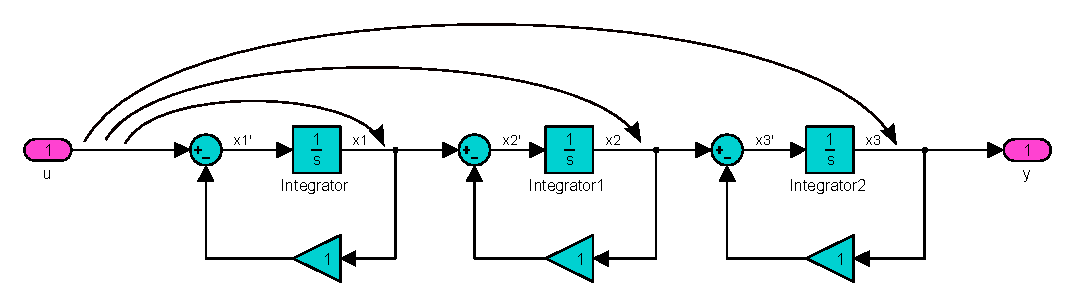
\includegraphics[width=1.00\textwidth]{03_Grafiken/Steuerbarkeit.pdf}
	\caption{Principle of controllability}
	\label{fig:Steuerbarkeit}
\end{figure}

The second term mentioned, is observability. It is very similar to the controllability, but it declares whether each state variable has influence on the output of the system.

\begin{align}\label{Q_b}
	Q_b = \left[c^T\ \  c^T*A\ \ c^T*A^2\ \ \cdots\ \ c^T*A^{n-1}\right]^T
\end{align}

The condition according to Kalman is very akin to the condition for controllability - the observability matrix $Q_b$ \myeqref{Q_b} must be full rank of the system. The rank of the $Q_b$ matrix in this example is three - so each state is observable. Figure \ref{fig:Beobachtbarkeit} shows the observability graphical.

\begin{figure}
	\centering
		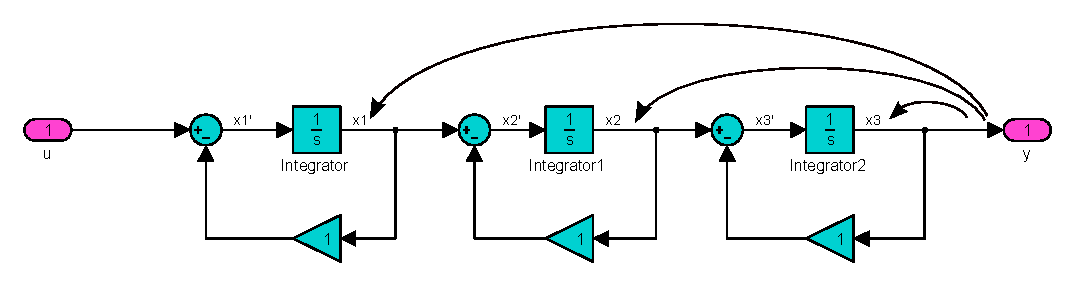
\includegraphics[width=1.00\textwidth]{03_Grafiken/Beobachtbarkeit.pdf}
	\caption{Principle of observability}
	\label{fig:Beobachtbarkeit}
\end{figure}



\pagestyle{fancy}
\subsection{State space controller}

In chapter \ref{chapter_StateSpace} the basic idea of the state space representation is explained. This chapter deals with the part, controlling the process of \myfigref{fig:simpleProcess}. 

But how to do that?

One possibility is, to use several PI(D) controllers in an cascade control architecture, but - in this case - a state space controller is the candidate. The fundamental idea of this controller is, to feed back all required internal state variables. In the feedback of each state variable, there has to be a specific factor. The method used in this project to determine these factors, is the pole placement (chapter \ref{chapter_PolePlace}). In order to be able to develop a state space controller for a process - as the dynamics of the quadrocopter - it is necessary, that the process is controllable.

How does a state space controller for the process of \myfigref{fig:simpleProcess} look like?

\begin{figure}
	\centering
		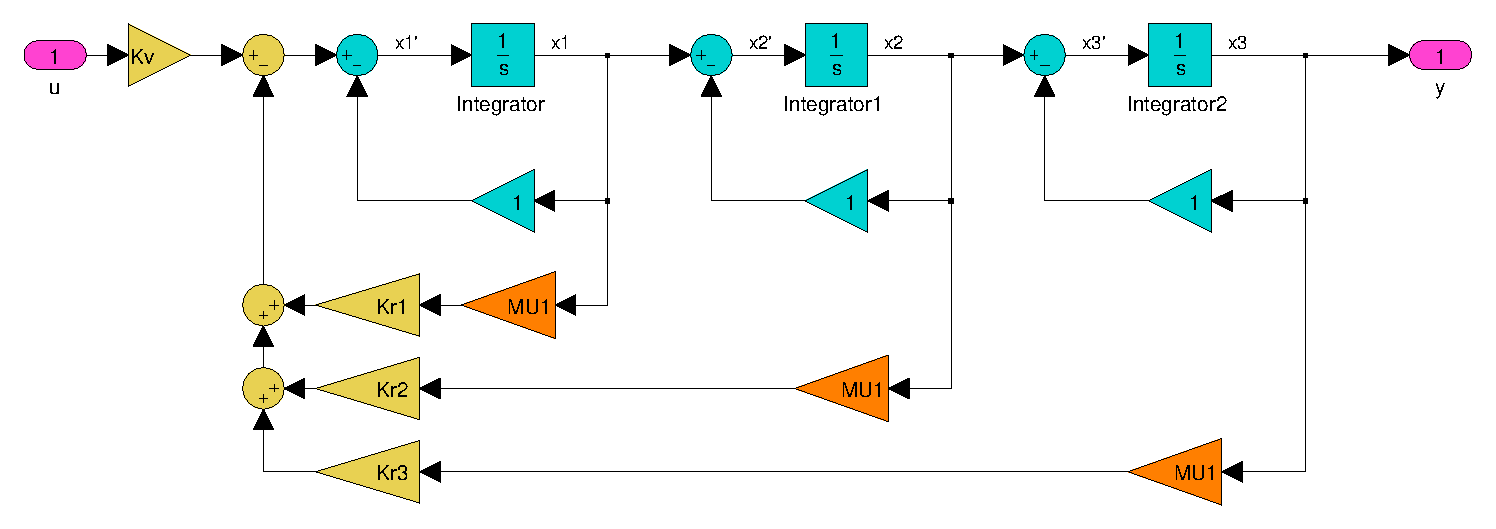
\includegraphics[width=1.00\textwidth]{03_Grafiken/simpleProcess_Controller.pdf}
	\caption{Simple process example including the state space controller}
	\label{fig:simpleProcess_Controller}
\end{figure}

There it is - the controller for the simple process of \myfigref{fig:simpleProcess}. The orange marked \textit{MUx} are the measuring converters, that are not important in this simple example. That is, why they are not described more precisely in this chapter. 
The controller is the whole part, marked in yellowish brown. On the one hand there are the feedback factors \textit{KRx}, on the other hand there is the pre-intensification factor \textit{Kv}. All in all, there are four independent parameters, which have to be calculated while designing the state space controller. For a MIMO system, chapter \ref{chapter_MIMO} deals with, there are much more independent parameters that have to be defined while designing.
As mentioned, the pre-intensification factor \textit{Kv} is one part of the controller. Its function is, to reduce the steady control deviation. How this factor and the other part of the state space controller, the feedback factors \textit{KRx}, are calculated, is described in the chapter \ref{chapter_PolePlace} pole placement.



\pagestyle{fancy}
\subsection{Pole placement}\label{chapter_PolePlacementIMPL}

There are two requirements, that have to be checked before starting with the pole placement. First one is, that the physical process, that shall be controlled, is available as a linear mathematical model - e.g in Simulink. The other one is, that this process is controllable. Chapter \ref{chapter_StateSpaceIMPL} deals with that fact. 

First of all it is necessary to check where the poles of the process are. This can be done with the following MATLAB code.

\begin{lstlisting}
	System = linmod('dynamics_reduced_without_motordelay');
	StateSpace = ss(System.a, System.b, System.c, System.d);
	eig(StateSpace) 
	pzmap(StateSpace)        
\end{lstlisting}

The output of the eig() function is:
\begin{lstlisting}
         0
    0.2378
   -0.2378
         0
         0       
\end{lstlisting}

And the pole/zero-map looks like that:
\begin{figure}
	\centering
		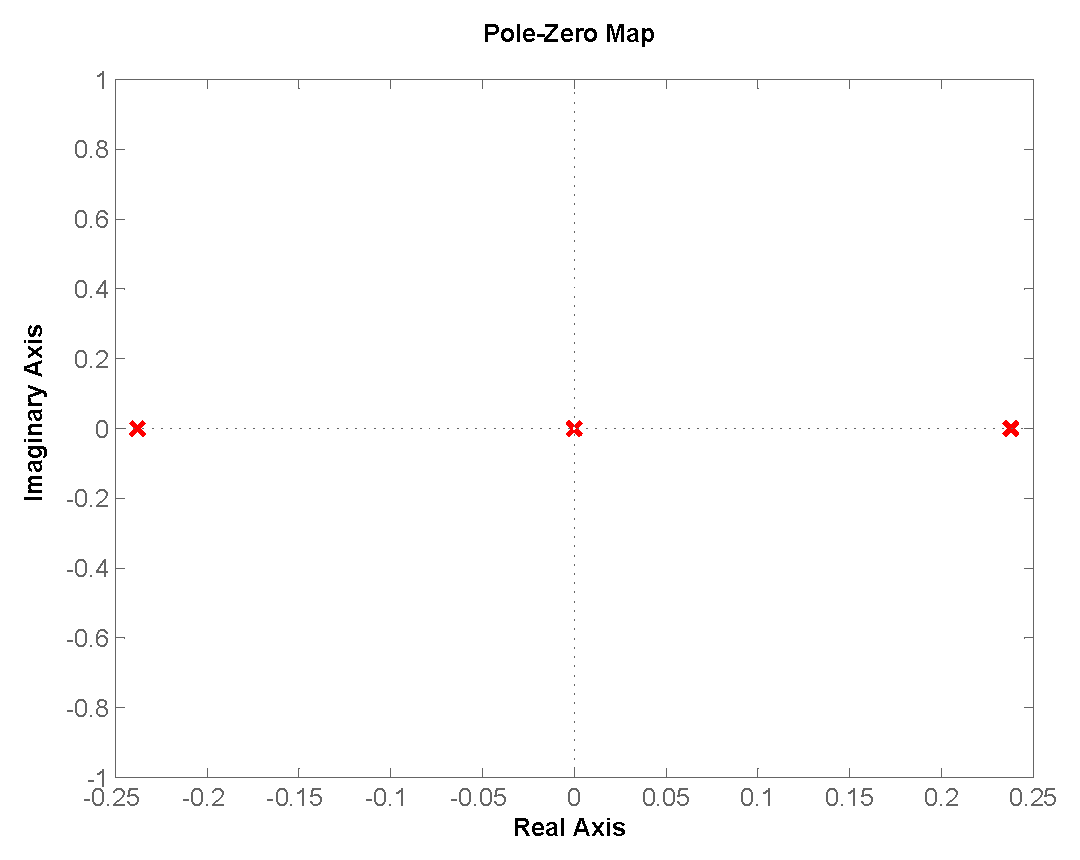
\includegraphics[width=0.70\textwidth]{03_Grafiken/PZmap_process.pdf}
	\caption{Pole/zero-map of the reduced quadrocopter process}
	\label{fig:PZmap_process}
\end{figure}


So there are five poles - three at zero, one at 0.2378 and one at -0.2378. This pole constellation - and consequently the process - is not stable, because one pole is at the right half-plane. So it is coercible necessary to use a controller for that process. The function of the pole placement is, to move at least the positive pole to the left half-plane. The three poles at zero are also not really nice, because they are not stable like the pole on the left half-plane. Poles on the imaginary axis can oscillate without damping. So the first requirement is, that all poles have to be moved to the left half-plane.
Next step is thinking about, to which values the poles should be moved. For an aircraft overshooting is not a good feature. So the second requirement is, that all poles have to stay at the real axis of the s-plane. And the third requirement is, that the poles, corresponding to the rates, have to be faster than those, belonging to the angles. 

To challenge all these requirements, the poles are moved to [-18 -5 -7 -10 -9]. Maybe these poles are too fast and they have to be moved to lower negative values. But it is not possible to know about that at this step of the development. Chapter \ref{chapter_TEST} deals with that circumstance.

\pagestyle{fancy}
\clearpage
\subsection{State observer}

In the simple example for a state space controller in figure \ref{fig:simpleProcess_Controller}, it was implied, that all state space variables can be measured. And these measured variables can be fed back in order to let the state space controller work. What if either a state variable can not be measured or the sensor costs too much to be economic?

David Gilbert Luenberger, working as professor at the Stanford University, invented a state observer called Luenberger observer. With this technique it is possible to use a state space controller, although not all state variable can be measured. 

\begin{figure}
	\centering
		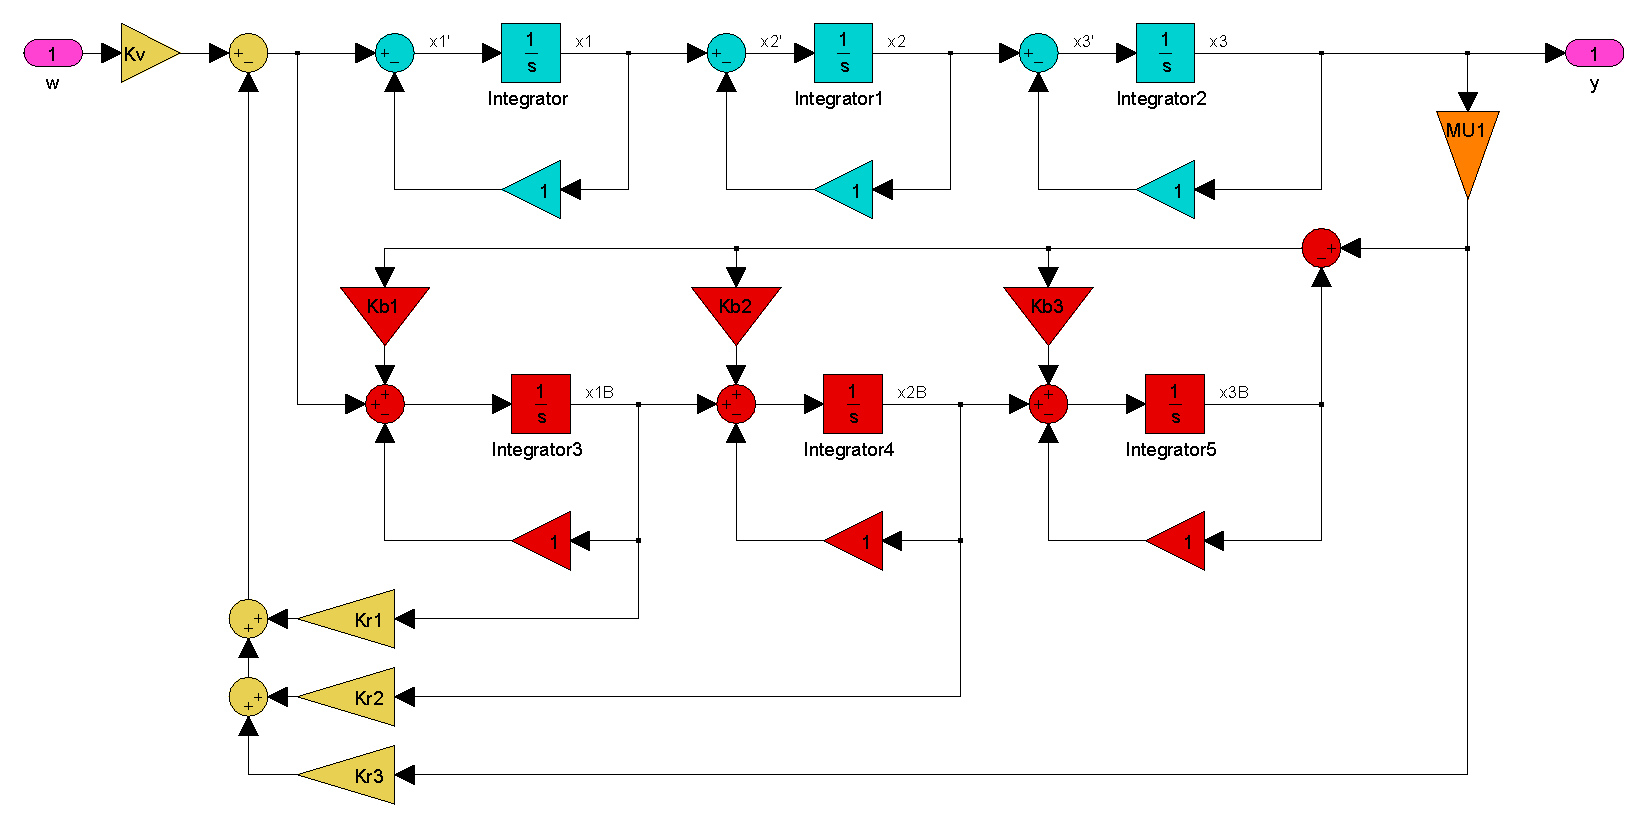
\includegraphics[width=1.00\textwidth]{03_Grafiken/simpleProcess_Controller_Observer.pdf}
	\caption{Simple process including a state space controller and an state observer}
	\label{fig:simpleProcess_Controller_Observer}
\end{figure}

In figure \ref{fig:simpleProcess_Controller_Observer} the state space controller is extended with an Luenberger observer. The observer is marked in red color. So, what exactly is shown there? To control the process with the standard state space controller, three measurement converters MUx are needed (\ref{fig:simpleProcess_Controller}). With the Luenberger observer, only one of them is required. In the example, there is a sensor for the output state variable. This state variable is fed back, just as common from the state space controller. But the other two state variables can not be measured, so the observer simulates the whole open loop process and implements this process in the controller. So the state variables \textit{x1B} and \textit{x2B} are fed back and if the observer poles are fast enough, the state space controller itself will not notice, that these state variables are not the original ones. These values are only estimated values but very good ones. To correct and stabilize the values of the observer, the measured value \textit{x3} is injected in the process and moves the simulated process in the right direction. This correcting works with the observer feedback factors \textit{Kbx}. 

Based on the fact, that the state space controller for the quadrocopter will not require an observer, this chapter will not be enlarged. 

\pagestyle{fancy}
\subsection{MIMO-Systems}\label{chapter_MIMO}

This part of the research paper reveals the secret of MIMO-Systems. MIMO is the abbreviation for 'Multiple Input Multiple Output'. All chapters before this one, deal with the simple 'SISO' example. But the quadrocopter process is very complex and like chapter \ref{chapter_VARIABLES} explains, there are three important control variables, that have to be controlled in parallel. And again - in this chapter - a little example for a MIMO system is explained, before the complex quadrocopter system is presented in the next chapter.

\begin{figure}
	\centering
		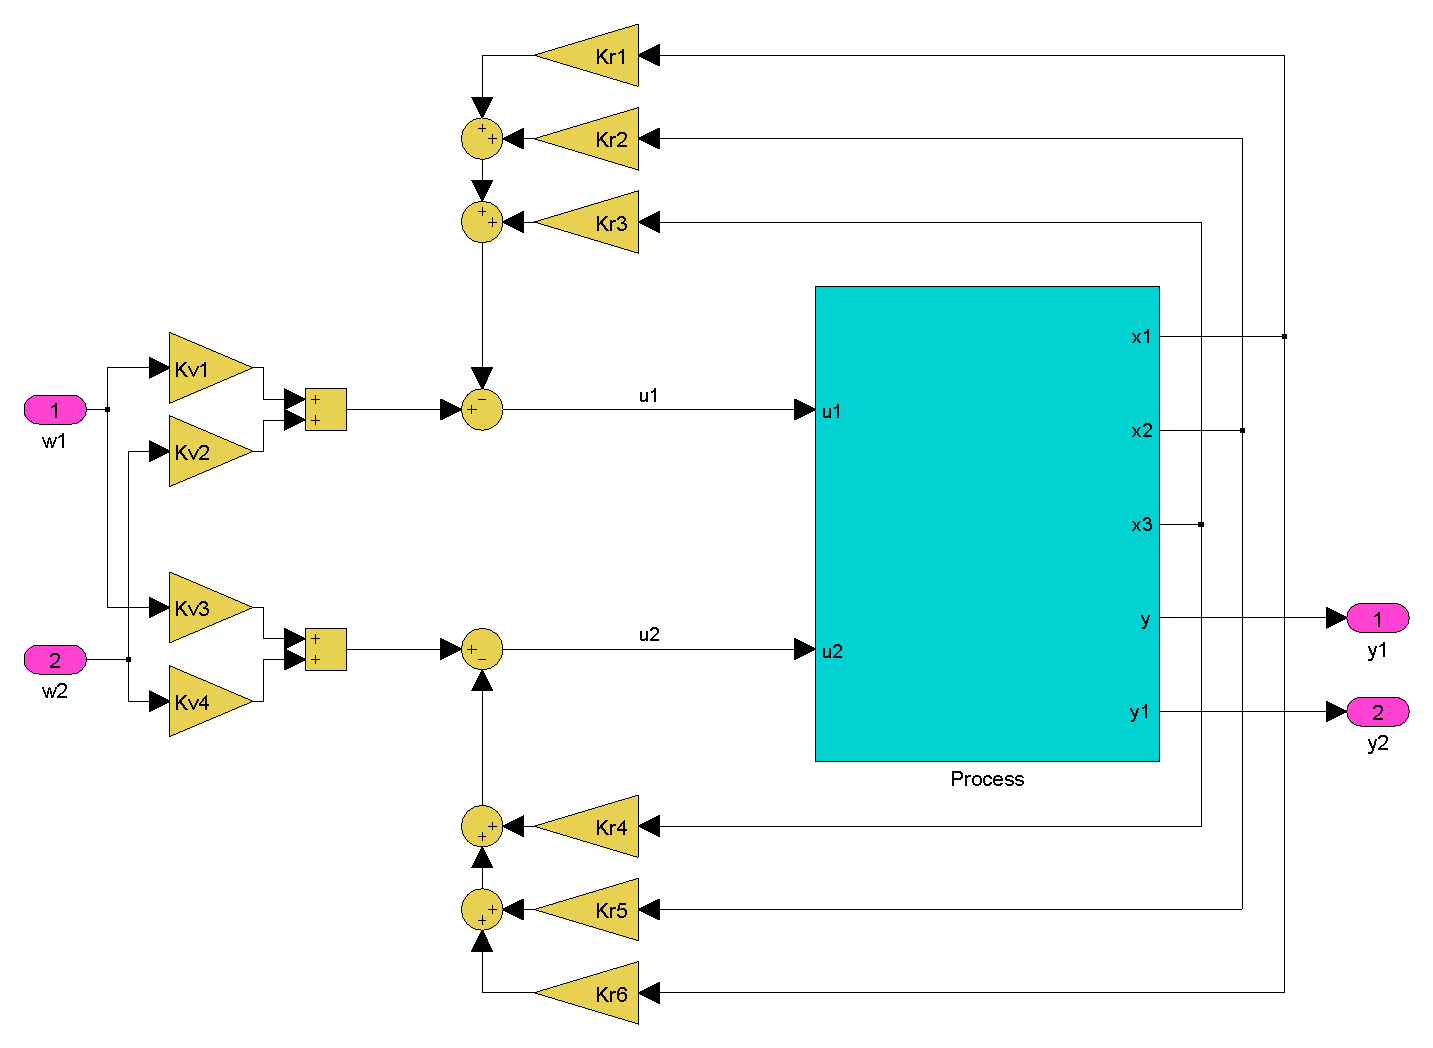
\includegraphics[width=1.00\textwidth]{03_Grafiken/MIMOprocess_controller.pdf}
	\caption{Principle model of a third order MIMO process including a state space controller}
	\label{fig:MIMOprocess_controller}
\end{figure}

Now in figure \ref{fig:MIMOprocess_controller} there is a simple MIMO-System. What exactly happens in the 'process-block' is not important, but there are two inputs \textit{u1} and \textit{u2}. Also, there are five outputs - three measured state variables \textit{x1}, \textit{x2} and \textit{x3} and the two outputs \textit{y1} and \textit{y2}. The state space controller, marked in yellowish brown, is a bit more complex than a state space controller for a SISO-System. So - how to calculate the state variable feedback factors and the pre-intensification factors now? Interesting answer, it is the same for MIMO-System as for SISO-Systems. The only thing is - it is more complex, because of more matrix equations, but those matrix equations are not the problem - therefore MATLAB is the tool.


 % chapter about the theory of the state space and controller
\clearpage %neue Seite erzwingen

\pagestyle{fancy}
\section{Design and implementation using MATLAB/Simulink}\label{chapter_DESIGN_AND_IMPL}

\pagestyle{fancy}
\subsection{Approach}\label{chapter_Approach}

At this point, all basics about the quadrocopter itself, the existing MATLAB Simulink model and about state space controlling should be clear. This chapter deals with the main part of what was developped in this research paper. 

\begin{figure}
	\centering
		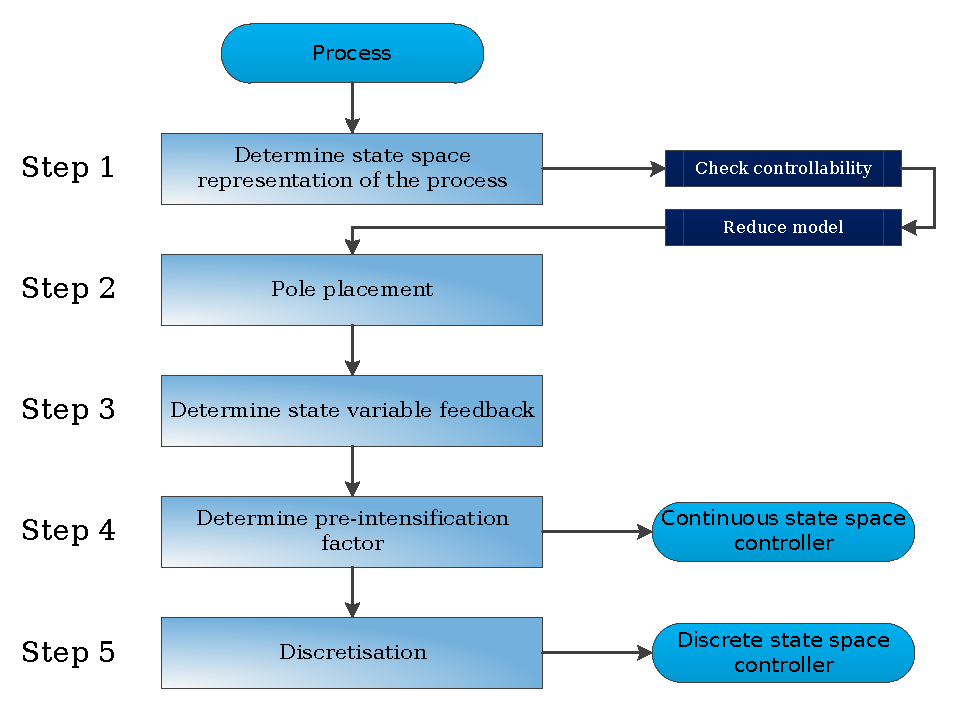
\includegraphics[width=1.00\textwidth]{03_Grafiken/Abstract.pdf}
	\caption{The five development steps}
	\label{fig:Abstract}
\end{figure}

To develop the state space controller the 'Five Steps', as they are named in the script of Prof.Kull (\cite{bib:KULL}), are used (figure \ref{fig:Abstract}). These steps are represented by the following sections. First step is to determine the state space representation of the process and check the controllability. Maybe it is necessary to reduce the model of the process. Thereafter, in the second step, the poles have to be placed in a wise order. In step three the state variable feedback factors for this specific pole constellation has to be calculated. Further on in step four, the corresponding pre-intensification factors must be estimated. After these four steps, the continuous state space controller for the MATLAB Simulink simulation and the basis for the implementation in C is completed. But to implement the controller into the quadrocopter - means in C - a discretization maybe is needed. The next chapter deals with that circumstance.

There are several reasons why MATLAB and MATLAB Simulink are used as development and simulation tool. One point is, that the cornerstone was implemented in MATLAB (chapter \ref{chapter_MATLAB_MODEL}). Another point is the uniqueness of MATLAB and MATLAB Simulink to combine all of the mentioned development steps in one tool. Even the HIL-Tests can be performed in this tool.
In the following sections the purpose, of why using MATLAB, will become clear.

\pagestyle{fancy}
\subsection{State space representation}\label{chapter_StateSpaceIMPL}

As mentioned in the chapter \ref{chapter_Approach}, first step in developing the state space controller is, to analyze the process of the quadrocopter. This process is introduced and explained in chapter \ref{chapter_DYNAMICS_BLOCK}. Chapter \ref{chapter_StateSpace} explains the basic knowledge about state space representation, needed in this chapter. Figure \ref{fig:MATLAB Dynamics Sections} shows the process of the quadrocopter. 

First of all it is necessary to find out, which part of the process is really needed to control the quadrocopter. So the earthframe part (blue) of the quadrocopter can be eliminated. 
Figures \ref{fig:MATLAB Dynamics1} and \ref{fig:MATLAB Dynamics2} are showing, how the remain looks like. That is only the bodyframe part of the process. And this part, is that one, the state space controller has to deal with.

\subsubsection{Controllability}\label{chapter_controllabilityIMPL}

Now the part of the process, that has to be controlled, is filtered out. Next step is, to check whether the process is controllable or not. To do so, the rank of the controllability matrix has to be the same as the number of state variables in the process. The easiest way to prove the controllability is, to use the ctrb() command in MATLAB. It returns the rank of the controllability matrix, which has to be compared with the number of state variables. With the linmod() function, it is possible to get the state space matrices of a Simulink model. 

Like figures \ref{fig:MATLAB Dynamics1} and \ref{fig:MATLAB Dynamics2} are showing, there are nine state variables that have to be controlled. These nine state variables, are the four motor delays (\ref{chapter_GREEN_SECTION}), the rate and the angle of phi, the rate and the angle of theta and the rate of psi. The angle of psi is not important, because it need not be controlled.

\begin{lstlisting}
	System = linmod('dynamics_reduced');
	StateSpace = ss(System.a, System.b, System.c, System.d);
	rank(ctrb(StateSpace))  
	% ans = 4                 
\end{lstlisting}

As the code snippet reveals, only four of the nine state variables can be controlled. Now there are two options to choose from. One is, to cancel the development process of the state space controller. But that is not the engineers way. The other option is, to continue reducing the model to gain full controllability. The next section deals with that.

\subsubsection{Model reduction}\label{chapter_ModelReductionIMPL}

The already reduced process without the earthframe part, is not controllable (chapter \ref{chapter_controllabilityIMPL}). So there is need to reduce the model once again, but all remaining parts of the model are needed to construct the state space controller. In this stage, the reduced process has to be examined very carefully. Looking at the delay in the four motors of the process, reveals, that there is only one millisecond delay in each motor (figure \ref{fig:motorWithDelay}).

\begin{figure}
	\centering
		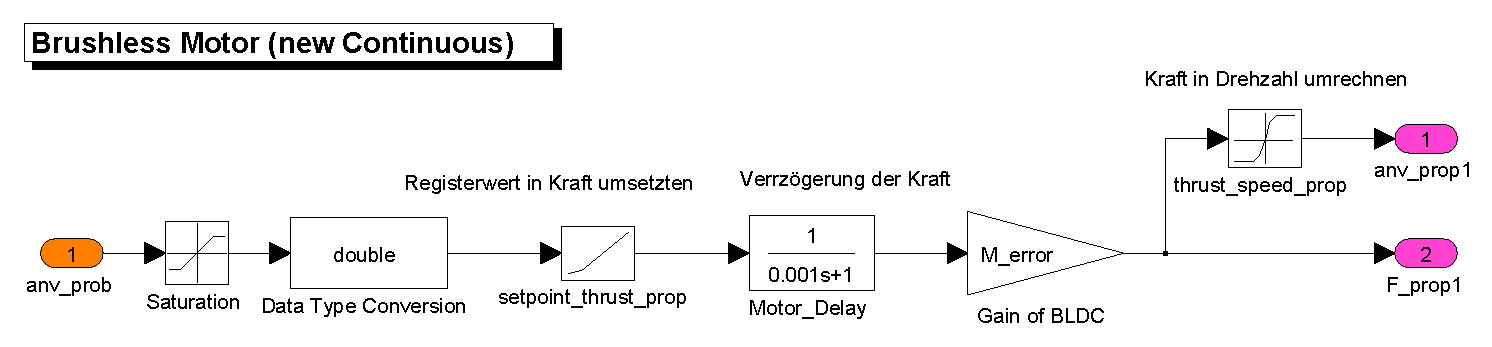
\includegraphics[width=1.00\textwidth]{03_Grafiken/motorWithDelay.pdf}
	\caption{Model of one motor including the time delay}
	\label{fig:motorWithDelay}
\end{figure}

In comprehension to the delays in each of the processes remaining integrators, the one millisecond can be disregarded (figure \ref{fig:motorWithoutDelay}). Now the same code, already used in chapter \ref{chapter_controllabilityIMPL}, has to run again, to check the controllability.

\begin{figure}
	\centering
		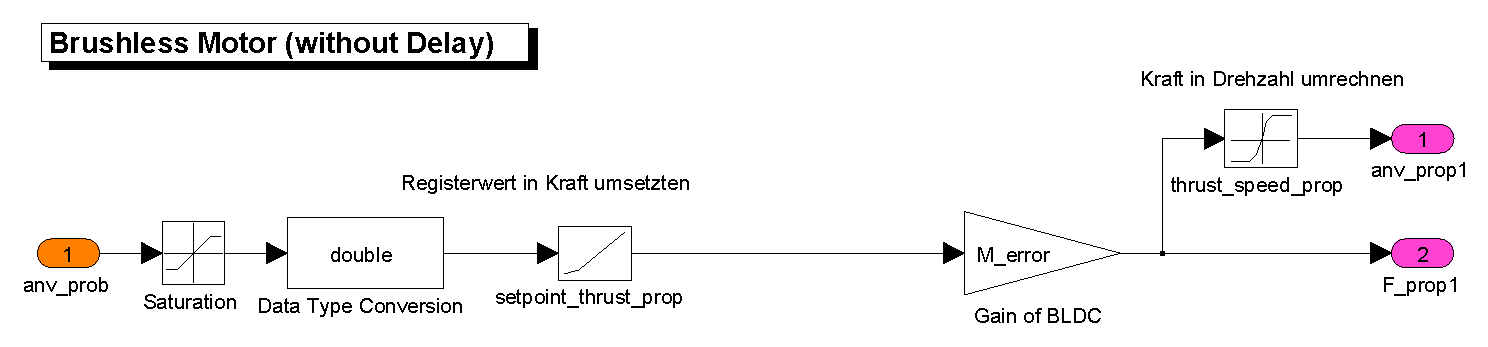
\includegraphics[width=1.00\textwidth]{03_Grafiken/motorWithoutDelay.pdf}
	\caption{Model of one motor without the time delay}		
	\label{fig:motorWithoutDelay}
\end{figure}


\begin{lstlisting}
	System = linmod('dynamics_reduced_without_motordelay');
	StateSpace = ss(System.a, System.b, System.c, System.d);
	rank(ctrb(StateSpace))  
	% ans = 5                 
\end{lstlisting}

Now the rank of the controllability matrix is five. That is the right number of controllable state variables, because the four motor delays are removed and so there are only five state variables remaining. At this point of the development it is not sure, if the state space controller, developed for this model without motor delay, will work later on with the process including the motor delay.


\subsubsection{Observability}\label{chapter_observabilityIMPL}

Just a few words about the observability of the process. Five states are controllable - the rate of phi, theta, psi and the angle of phi and theta. Chapter \ref{chapter_SENSORS} shows the sensors, used in the quadrocopter. For each of the five state variables there is a sensor. That is the reason, why no observer is needed in this project, but - maybe interesting for a further project - the observability of the system is given. So it might be possible to reduce the number of sensors and develop an observer instead. The following code snippet shows that.

\begin{lstlisting}
	System = linmod('dynamics_reduced_without_motordelay');
	StateSpace = ss(System.a, System.b, System.c, System.d);
	rank(obsv(StateSpace)) 
	% ans = 5                 
\end{lstlisting}


\pagestyle{fancy}
\subsection{Simulink}\label{chapter_SimulinkIMPL}

Finally, before calculating the state variable feedback factors in the next chapter, it is advisable to create a dummy state space controller in Simulink. Therefore it is necessary to know what the actuating variables are. Figure \ref{fig:Remote control stimuli} shows these input variables named \textit{phi\_set}, \textit{theta\_set}, \textit{rpsi\_set} and \textit{thrust\_set}. The thrust is controlled directly by the remote control and does not have to be controlled in the quadrocopter. The other three variables are the set variables that must be controlled internal. \\
In addition the input of the process - thus the output of the controller - has to be defined. As figure \ref{fig:Controller block} shows, the outputs of the controller block are the desired pseudo forces for the four motors of the quadrocopter.

The three set variables calculated by the controller and the thrust are mixed together and four pseudo forces are the result. This is very easy to understand - for example \textit{phi\_set} tells, that the quadrocopter shall move to the left, so the left motor is slowed down and the right one is accelerated. 

\begin{figure}
	\centering
		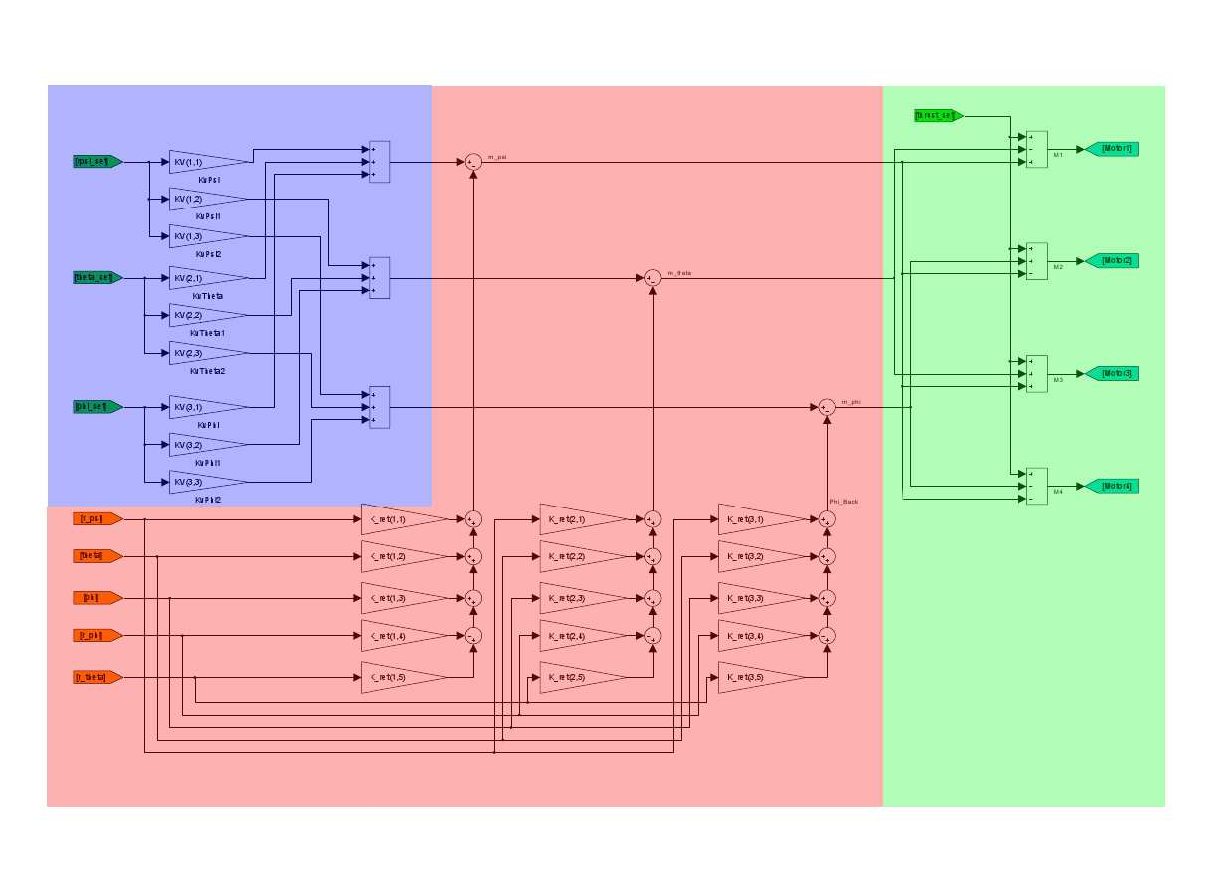
\includegraphics[width=1.00\textwidth]{03_Grafiken/SS_overview.pdf}
	\caption{Overview over the whole state space controller}
	\label{fig:SS_overview}
\end{figure}

Figure \ref{fig:SS_overview} shows the complete state space controller. In the following sub chapters the red and blue part are explained. 

\begin{figure}
	\centering
		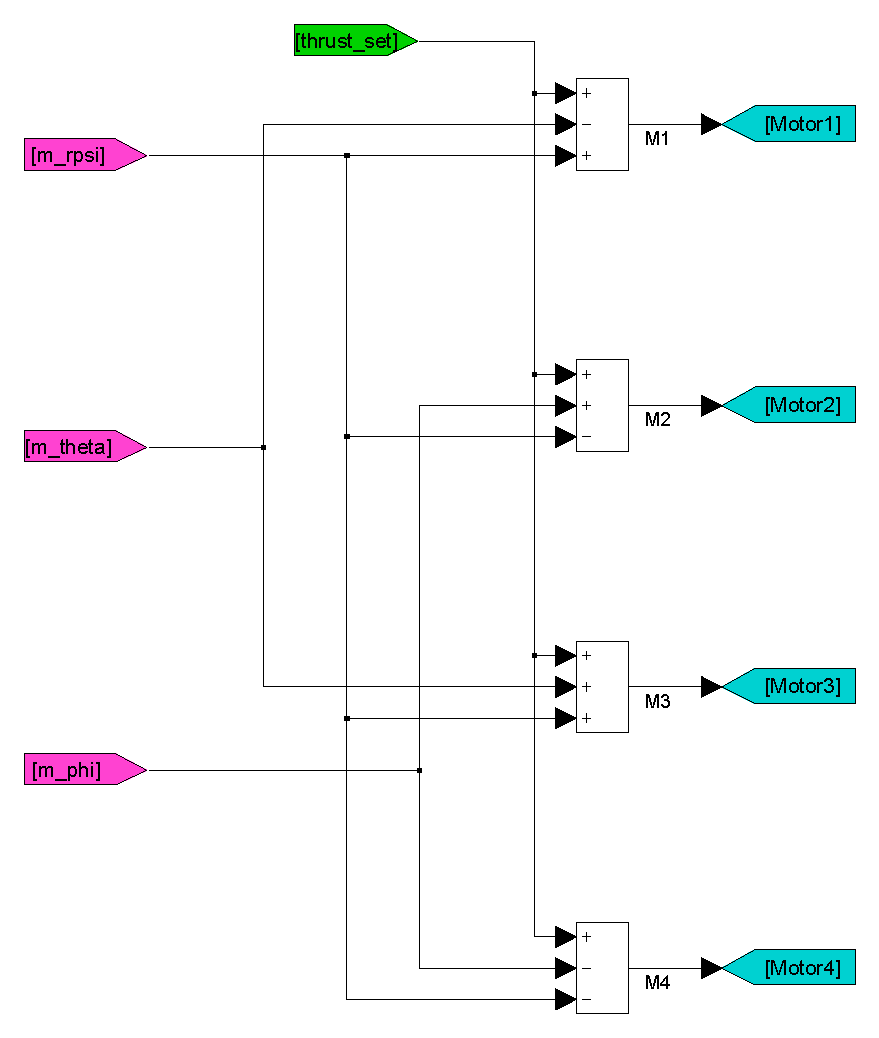
\includegraphics[width=0.60\textwidth]{03_Grafiken/SS_Trafo.pdf}
	\caption{Transformation of the set values to pseudo forces}
	\label{fig:SS_Trafo}
\end{figure}

Figure \ref{fig:SS_Trafo} shows this green part in detail. This part is something like a transformation from set values, for every moving direction of the quadrocopter, to pseudo forces. Giving more \textit{thrust}, all four motors are accelerated and the result is, that the quadrocopter raises. Changing \textit{m\_rpsi} means, accelerating two motors and decelerating the other two. In this case, the quadrocopter is yawing. For \textit{m\_theta} and \textit{m\_phi} it is both nearly the same. One motor is accelerated and the opposing motor is decelerated. The quadrocopter flies in direction of the decelerated motor. \\
For sure, all combinations of these four input values are possible. 

\pagestyle{fancy}
\subsection{Pole placement}\label{chapter_PolePlacementIMPL}

There are two requirements, that have to be checked before starting with the pole placement. First one is, that the physical process, that shall be controlled, is available as a linear mathematical model - e.g in Simulink. The other one is, that this process is controllable. Chapter \ref{chapter_StateSpaceIMPL} deals with that fact. 

First of all it is necessary to check where the poles of the process are. This can be done with the following MATLAB code.

\begin{lstlisting}
	System = linmod('dynamics_reduced_without_motordelay');
	StateSpace = ss(System.a, System.b, System.c, System.d);
	eig(StateSpace) 
	pzmap(StateSpace)        
\end{lstlisting}

The output of the eig() function is:
\begin{lstlisting}
         0
    0.2378
   -0.2378
         0
         0       
\end{lstlisting}

And the pole/zero-map looks like that:
\begin{figure}
	\centering
		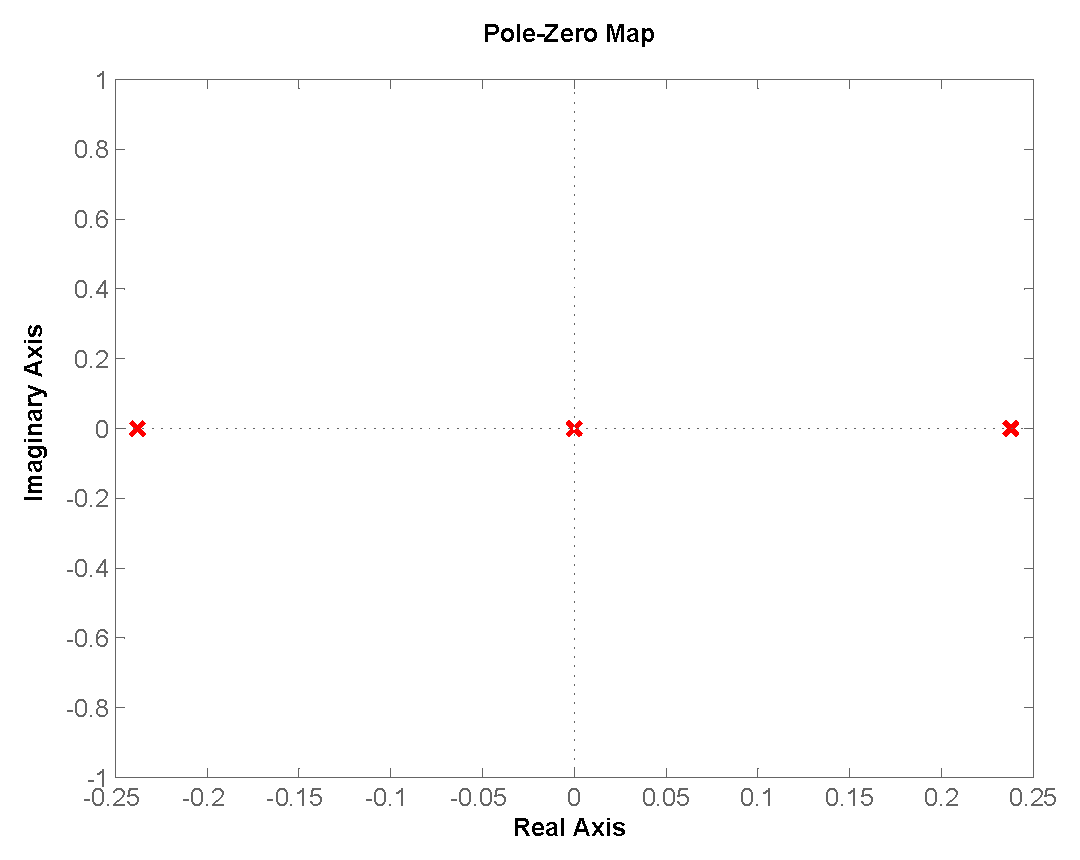
\includegraphics[width=0.70\textwidth]{03_Grafiken/PZmap_process.pdf}
	\caption{Pole/zero-map of the reduced quadrocopter process}
	\label{fig:PZmap_process}
\end{figure}


So there are five poles - three at zero, one at 0.2378 and one at -0.2378. This pole constellation - and consequently the process - is not stable, because one pole is at the right half-plane. So it is coercible necessary to use a controller for that process. The function of the pole placement is, to move at least the positive pole to the left half-plane. The three poles at zero are also not really nice, because they are not stable like the pole on the left half-plane. Poles on the imaginary axis can oscillate without damping. So the first requirement is, that all poles have to be moved to the left half-plane.
Next step is thinking about, to which values the poles should be moved. For an aircraft overshooting is not a good feature. So the second requirement is, that all poles have to stay at the real axis of the s-plane. And the third requirement is, that the poles, corresponding to the rates, have to be faster than those, belonging to the angles. 

To challenge all these requirements, the poles are moved to [-18 -5 -7 -10 -9]. Maybe these poles are too fast and they have to be moved to lower negative values. But it is not possible to know about that at this step of the development. Chapter \ref{chapter_TEST} deals with that circumstance.

\pagestyle{fancy}
\subsection{State variable feedback}\label{chapter_StateVariableFeedbackIMPL}

It is no problem for a state space controller to move the poles wherever the engineer wants them to go. How to do this by hand is explained in chapter \ref{chapter_PolePlace}. For this much more complicate process MATLAB is used. In chapter \ref{chapter_PolePlacementIMPL} the decision to move the poles to [-18 -5 -7 -10 -9] is made. As mentioned, MATLAB is used to find the state variable feedback factors needed by the state space controller to move the poles to the specific position. The following code calculates them.

\begin{lstlisting}
System = linmod('dynamics_reduced_without_motordelay');
StateSpace = ss(System.a, System.b, System.c, System.d);
K_ret = place(System.a, System.b, [-18 -5 -7 -10 -9]);     
\end{lstlisting}

The function place() calculates the state variable feedback factors. The result is:

\begin{align}\label{eq:feedback}
\bordermatrix[{[]}]{
	  				&  rpsi & theta & phi & rphi & rtheta \cr
rpsi\_set 	&  7.27 & 0 & -0.57 & -0.07 & 0.03 \cr
theta\_set	&  0.76 & 79.36 & 0.03 & 0 & 20.28 \cr
phi\_set		& 0 & 0 & 65.05 & 15.80 & 0 \cr
}
\end{align}

This matrix describes with which gain, which state variable has to be fed back. For example the state variable theta has to be fed back with a gain of 20.28 to the theta\_set path. 

There are two ways to prove, that the poles are moved to the estimated places. The first way is, to calculate the closed loop state matrix and the output matrix with the calculated feedback factors. The following code is doing that.

\begin{lstlisting}
A_CL = System.a - System.b * K_ret;
C_CL = System.c - System.d * K_ret;
Sys_ClosedLoop = ss(A_CL, System.b, C_CL, System.d);
eig(Sys_ClosedLoop)
\end{lstlisting}

The output of the eig() function are the poles that are passed to the place() function earlier. So it is clear, that the poles now are, where they should be. 

The second way is, to create the closed loop Simulink block diagram and get the state space representation with linmod(). At this point it is also possible to check weather it was a good or a bad decision to ignore the motor delays. The Simulink block diagram used in the following includes the whole state space controller and the process. Furthermore the motors with delay are used.

\begin{lstlisting}
S_CL = linmod('ControllerAndProcess');
SS_ClosedLoop = ss(S_CL.a, S_CL.b, S_CL.c, S_CL.d);
eig(SS_ClosedLoop)
\end{lstlisting}

And like expected, the result is:

\begin{lstlisting}
-9,66
-7,13
-4,99
-9,07
-18,47
-1016
-991
-977
-1000
\end{lstlisting}

The first five poles are the expected poles - not exactly, but a good result. The four remaining poles are those for the motor delays. So it is possible to see, that they do not really disturb the others, because they are very far away on the left side of the s-plane.


So how does this feedback look like in a Simulink block diagram? 

\begin{figure}
	\centering
		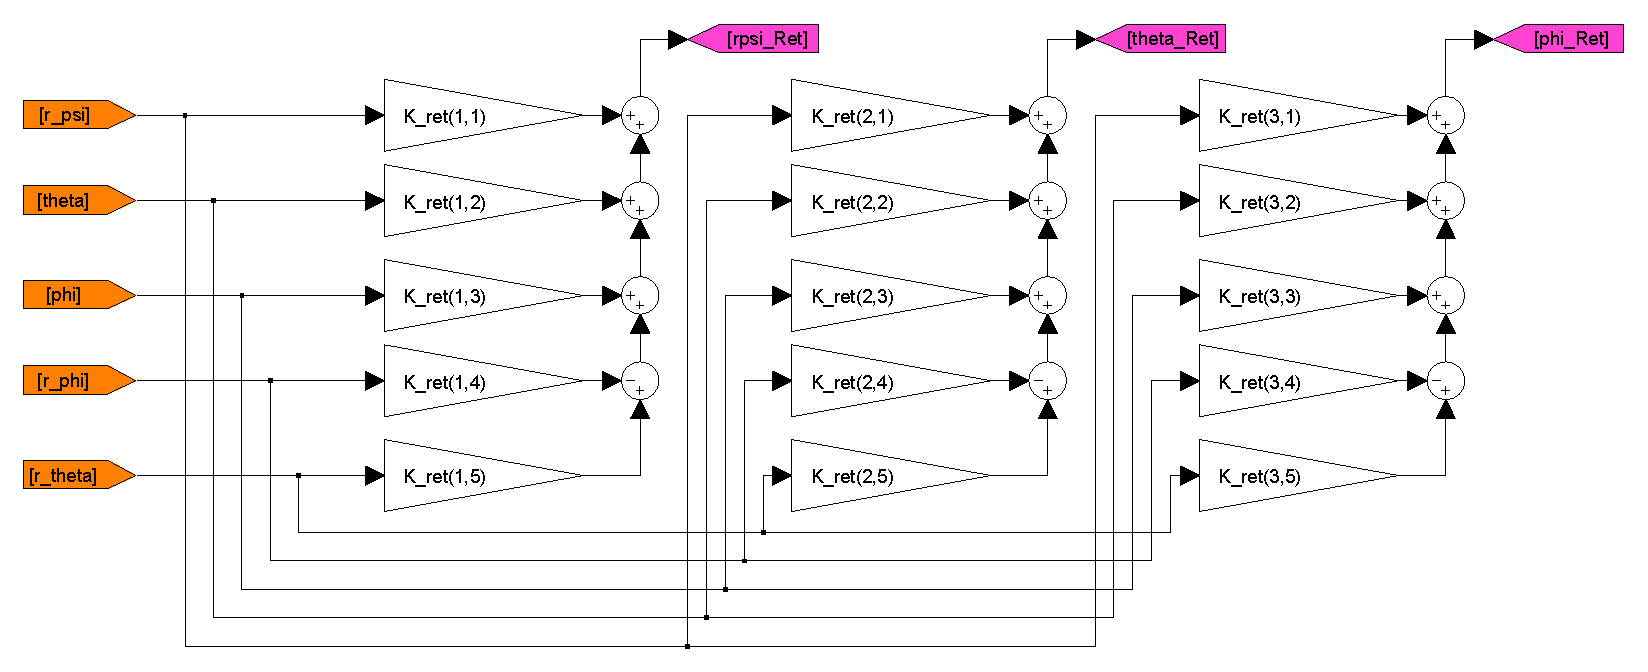
\includegraphics[width=1.00\textwidth]{03_Grafiken/SS_Feedback.pdf}
	\caption{Feedback part of the state space controller}
	\label{fig:SS_Feedback}
\end{figure}

Figure \ref{fig:SS_Feedback} shows the red part of the overview figure \ref{fig:SS_overview}. The input values marked orange, are the measured state variables of the process. The output values marked in magenta, are the added state variables with their specific feedback factors. The calculated matrix (\ref{eq:feedback}) can be written in the gain blocks in this diagram. Now there is maybe some unclarity, because some of those feedback factors are zero and even so there is a gain block for them. The reason is, that if the pole constellation is changed, these calculated values may change from zero to an important value. Another blur is the minus sign in the feedback factors for \textit{rphi}. The answer is very simple - the sensor, measuring this value, is build in the 'wrong way'. So all values have to be flipped.

\pagestyle{fancy}
\subsection{Control deviation}\label{chapter_controlDeviationIMPL}

After calculating the state variable feedback, the dynamic behavior of the quadrocopter is fine, but the quadrocopter will not fly. There is something missing - the pre-intensivication factors. In this MIMO system, each input variable \textit{rpsi\_set}, \textit{theta\_set} and \textit{phi\_set} influences each of the three control paths. But not in the same intensity. 

First, the set variables are standardized, so that the range of the input values from -128 to 128 now reaches from -0.75 to 0.75. This is necessary, because the angels \textit{theta} and \textit{phi} are calculated in rad and the stationary throughput is calculated being one. That means, a maximum angle of approximately 45\textdegree is reached. Maybe it sounds very little, but believe - it is not. The yaw rate \textit{rpsi} is calculated in $rad/s$ so this value of 0.75 (45\textdegree/s) sounds nice for that purpose, too. 

Calculating the pre-intensification factors is not very complex. The following little code snippet shows that.

\begin{lstlisting}
KV = -(System.c * A_CL^-1 * System.b)^-1;
KV = KV';             
\end{lstlisting}

The result is the following matrix.

\begin{align}\label{eq:kv}
\bordermatrix[{[]}]{
	  				&  rpsi\_Path & theta\_Path & phi\_Path \cr
rpsi\_set 	&  7.27 & -0,32 & 0 \cr
theta\_set	&  0 & 79.36 & 0 \cr
phi\_set		& -0,57 & 0,03 & 65.05 \cr
}
\end{align}

Looking closer at the matrix reveals that these factors are nearly the same as the state variable feedback factors.

The final step is the implementation in Simulink. This part is the red one in the overview figure \ref{fig:SS_overview}. 

\begin{figure}
	\centering
		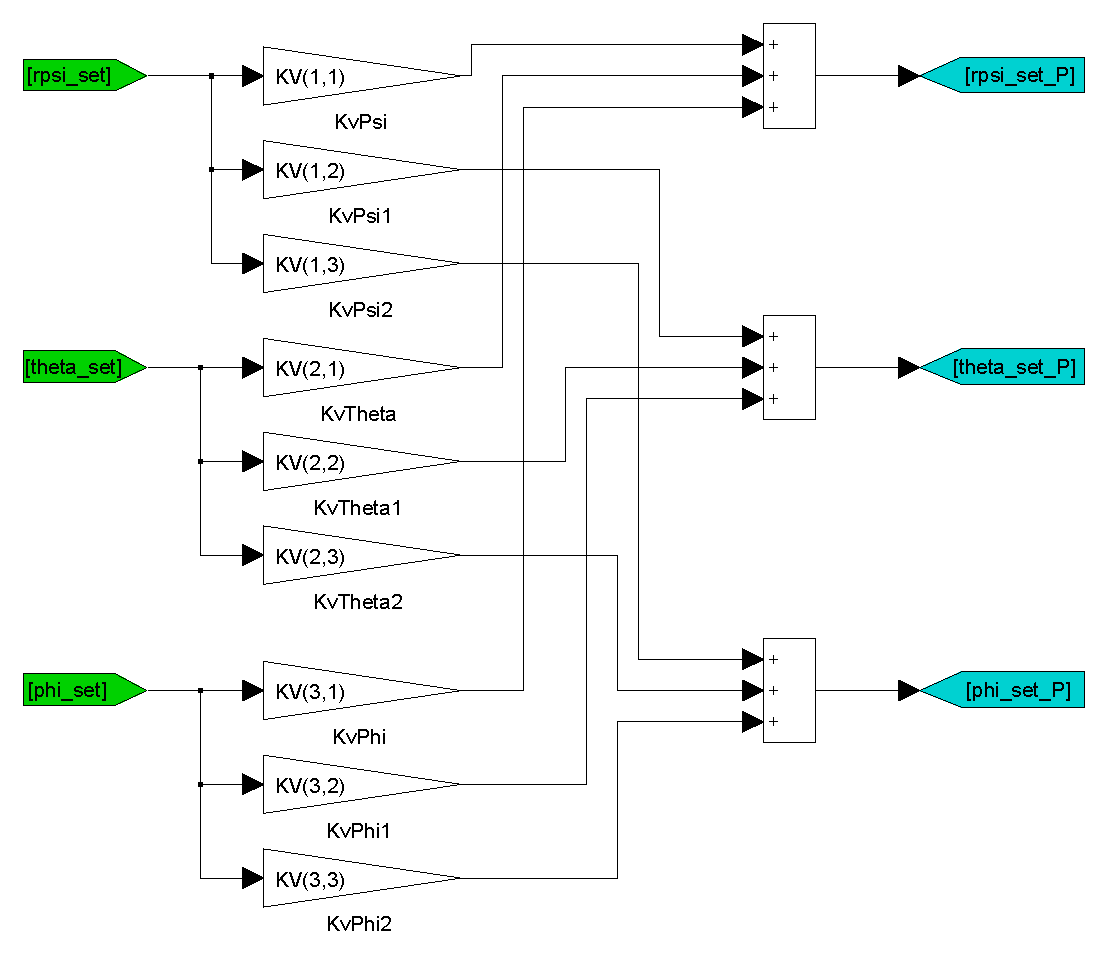
\includegraphics[width=0.80\textwidth]{03_Grafiken/SS_Pre.pdf}
	\caption{Pre-intensification factors for the different control paths}
	\label{fig:SS_Pre}
\end{figure}

Figure \ref{fig:SS_Pre} shows a detailed look at that part. The input values, marked green, are the standardized set values from the remote control. The output values, marked cyan, are the calculated set values for each path, but including the influence of the other set values.

At this step of development the continuous state space controller is finished as figure \ref{fig:Abstract} shows. The simulation results can be found in chapter (\ref{chapter_TEST}).
 % chapter about the design and the implementation in Matlab
\clearpage %neue Seite erzwingen

\pagestyle{fancy}
\section{Implementation in C}\label{chapter_IMPLC}

At the beginning of chapter \ref{chapter_DESIGN_AND_IMPL} figure \ref{fig:Abstract} shows, that for the implementation in C, the state space controller may have to be discretized. In this project it is not necessary to do so, because the fastest pole of the whole system is less than a tenth as fast as the sampling rate. That is an engineer's rule of thumb and therefore not explained in detail.

So the state space controller can directly be transfered from the Matlab/Simulink to the existing quadrocopter C project. In this quadrocopter software is an existing function called 'Controll'. This function is called cyclic every 5ms and calculates the new motor forces. So the only thing to change, implementing the state space controller instead of the PID controller, is, to write a new 'Controll' function.

The 'Controll' function can be found in the appendix (chapter \ref{chapter_CFUNC}). It is easy to understand the code, by looking at the C code and at the Matlab/Simulink model at the same time.

 % chapter about the testing (simulation & real copter)
\clearpage %neue Seite erzwingen

\pagestyle{fancy}
\section{Final tests}\label{chapter_TEST}

The subchapters in this chapter are dealing with the different steps of testing the state space controller. First, chapter \ref{chapter_REQUIREMENTS} collects the requirements, the system has to fulfill. Second, chapter \ref{chapter_SimulationTest} deals with the Matlab/Simulink simulation test. Third, chapter \ref{chapter_HILTest} deals with the HIL test and finally chapter \ref{chapter_RealCopterTest} deals with the tests, using the real quadrocopter.

\pagestyle{fancy}
\subsection{Requirements}\label{chapter_REQUIREMENTS}

In summary there are not many requirements, that really have to be fulfilled. Most of the requirements that are mentioned in this document in multiple chapters are imprecise or variable. This short chapter collects all the requirements to allow structured tests.

\begin{enumerate}
	\item The controller has to operate without of additional sensors.
	\item The transient effect should be fast 'enough'.
	\item There must not be overshooting of the controlled variables.
	\item The system has to be stable/must not be oscillating.
	\item The values of the controlled variables must be reasonable.
\end{enumerate}

Requirement No. 1 is already fulfilled, because with the existing sensors, it is possible, to measure all state variables, so no additional sensors are needed.
The following tests check the fulfillment of the other four requirements.


\pagestyle{fancy}
\subsection{Simulation test}\label{chapter_SimulationTest}

This chapter is about testing the Matlab/Simulink state space controller with the Matlab/Simulink process. Therefore the same control sequence of the remote input is used for the PID controller and the state space controller. A random sensor noise is enabled during the whole simulation time.

This sequence is:
\begin{enumerate}
\item{Start of simulation}
\item{At 2 seconds a \textit{phi} step to -0.35 rad (~-20 degree)}
\item{At 4 seconds a \textit{theta} step to 0.35 rad (~20 degree)}
\item{At 6 seconds a \textit{rpsi} step to 0.75 rad/s (~43 degree/s)}
\item{Start of simulation}
\end{enumerate}
 
After running this sequence (duration 10 seconds), there are several scopes used to check the result. Figures \ref{fig:Motor_PID} to \ref{fig:rpsi_PID} are showing the result, using the PID controller, figures \ref{fig:Motor2_SS} to \ref{fig:rpsi_SS} those, using the developed state space controller.

\begin{figure}
	\centering
		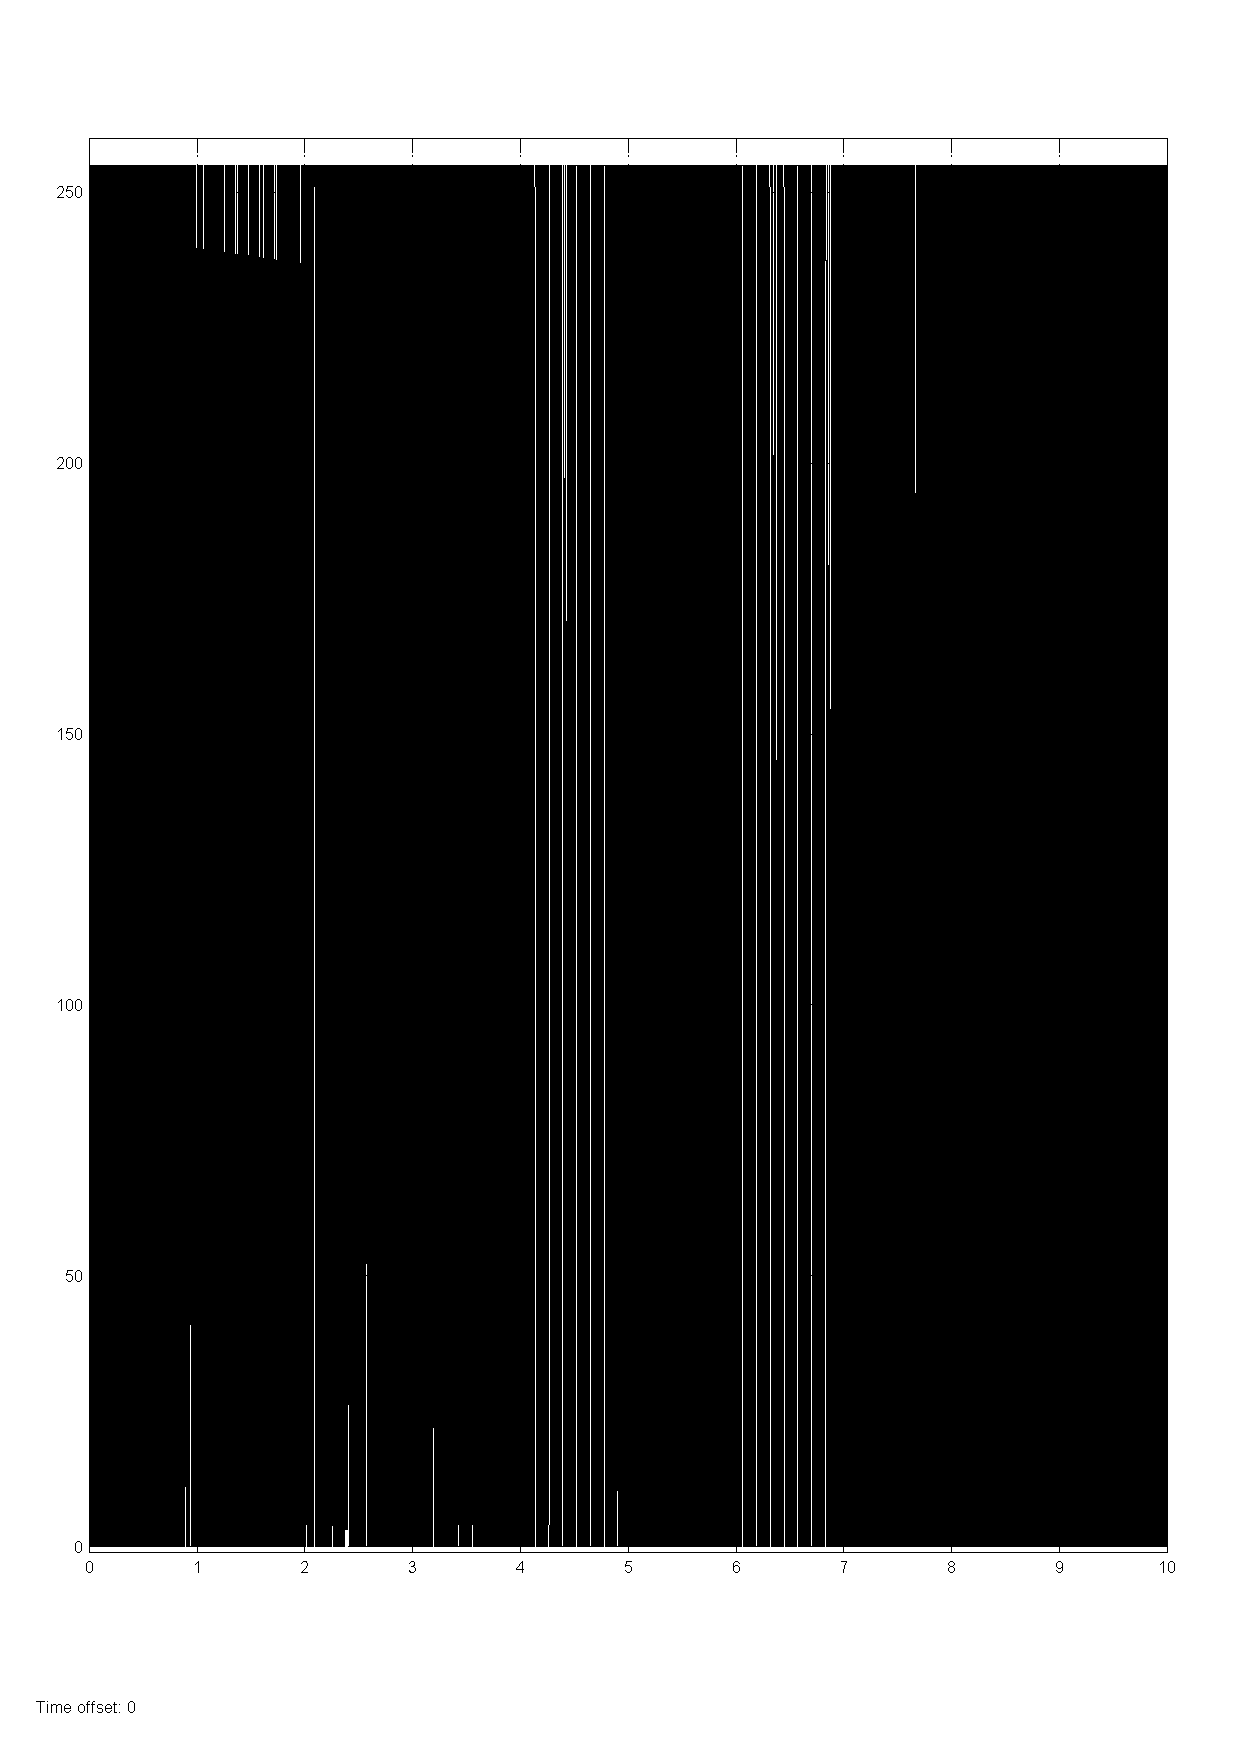
\includegraphics[width=0.3\textwidth]{03_Grafiken/Motor_PID.pdf}
	\caption{Set value for one motor using the PID controller}
	\label{fig:Motor_PID}
\end{figure}

Figure \ref{fig:Motor_PID} shows one of the four set values for the motor forces. That is no graphical error, but the PID controller pushes the actuating variables the whole time into the saturation of 255 and 0. Interestingly this strategy works, like the following figures are showing.

\begin{figure}
	\centering
		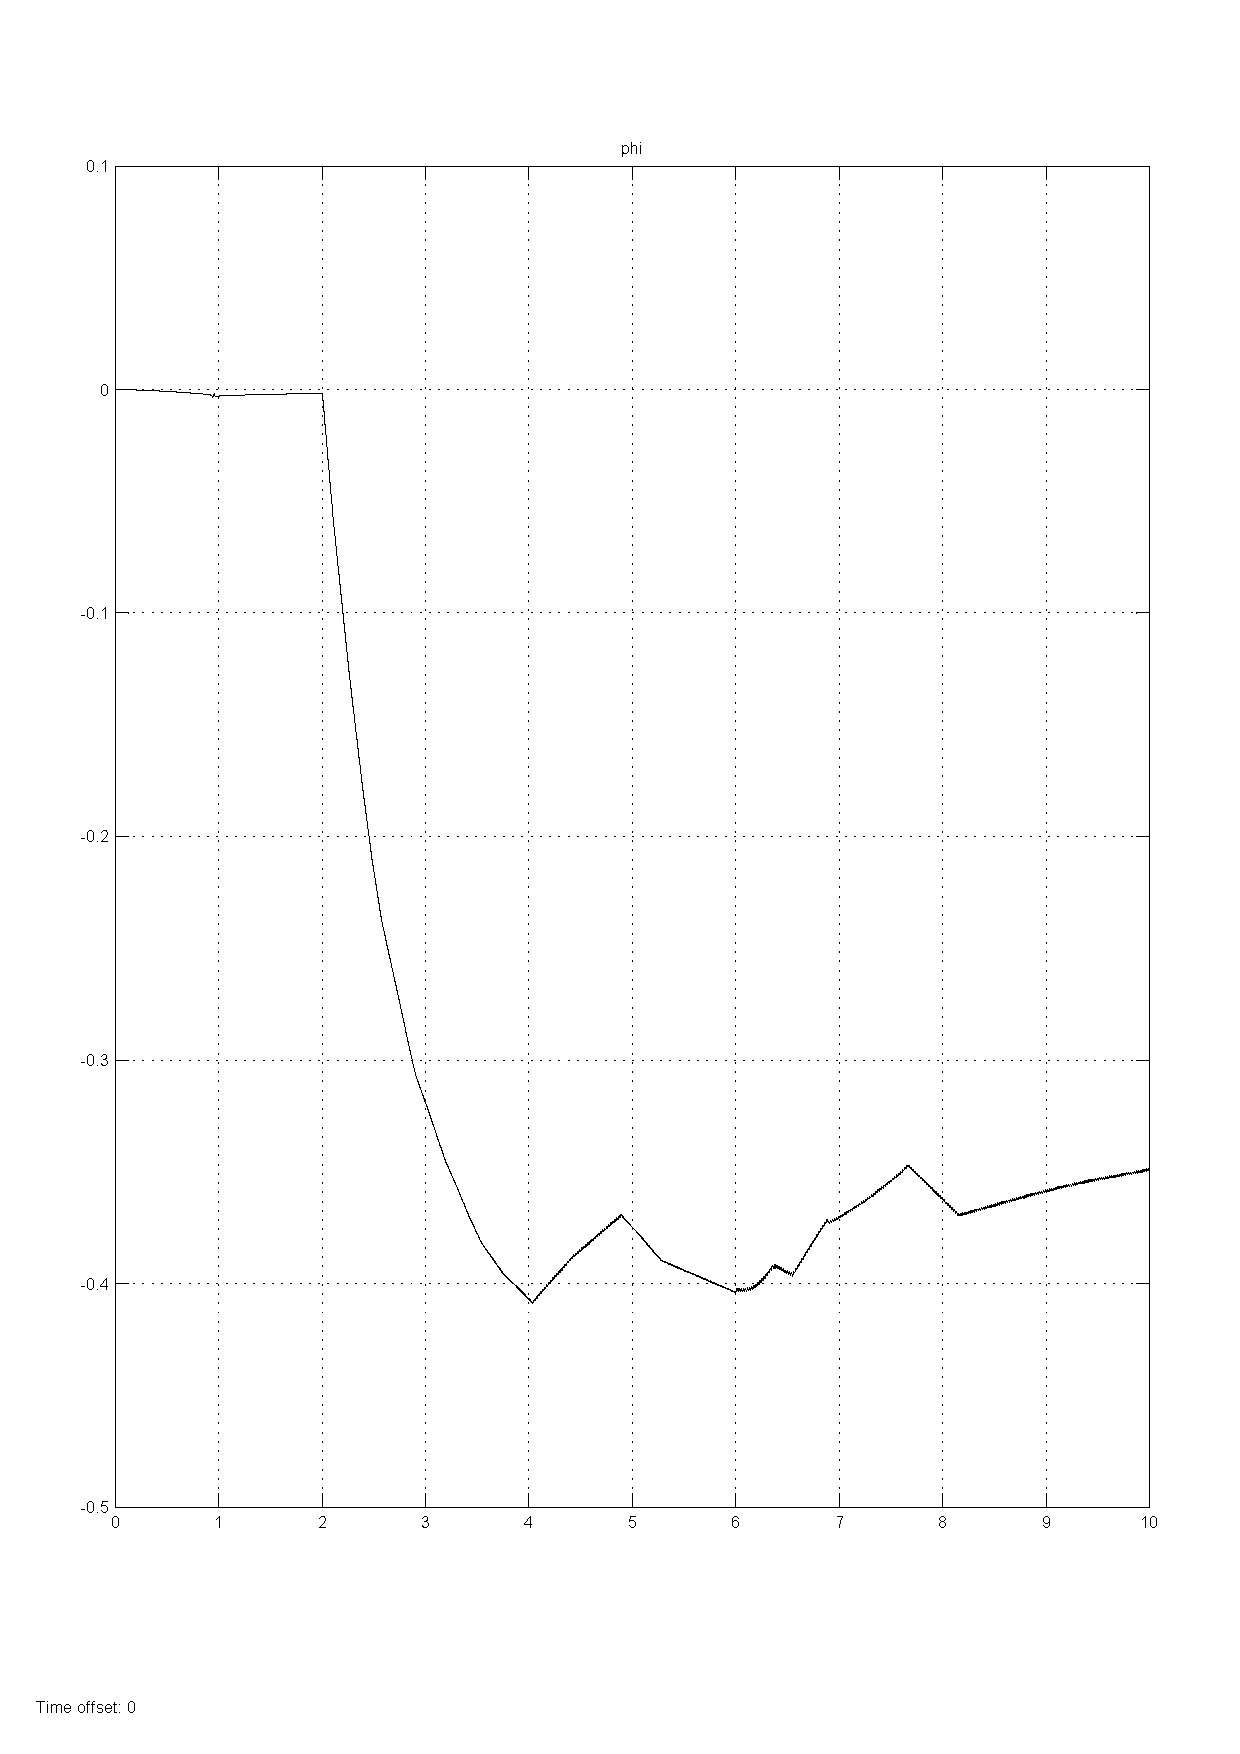
\includegraphics[width=0.8\textwidth]{03_Grafiken/phi_PID.pdf}
	\caption{Angle of phi using the PID controller}
	\label{fig:phi_PID}
\end{figure}

Figure \ref{fig:phi_PID} shows the angle of \textit{phi} after the whole sequence. The estimated angle is not hold stable. There are heavy influences at the time, the other two steps occur.

\begin{figure}
	\centering
		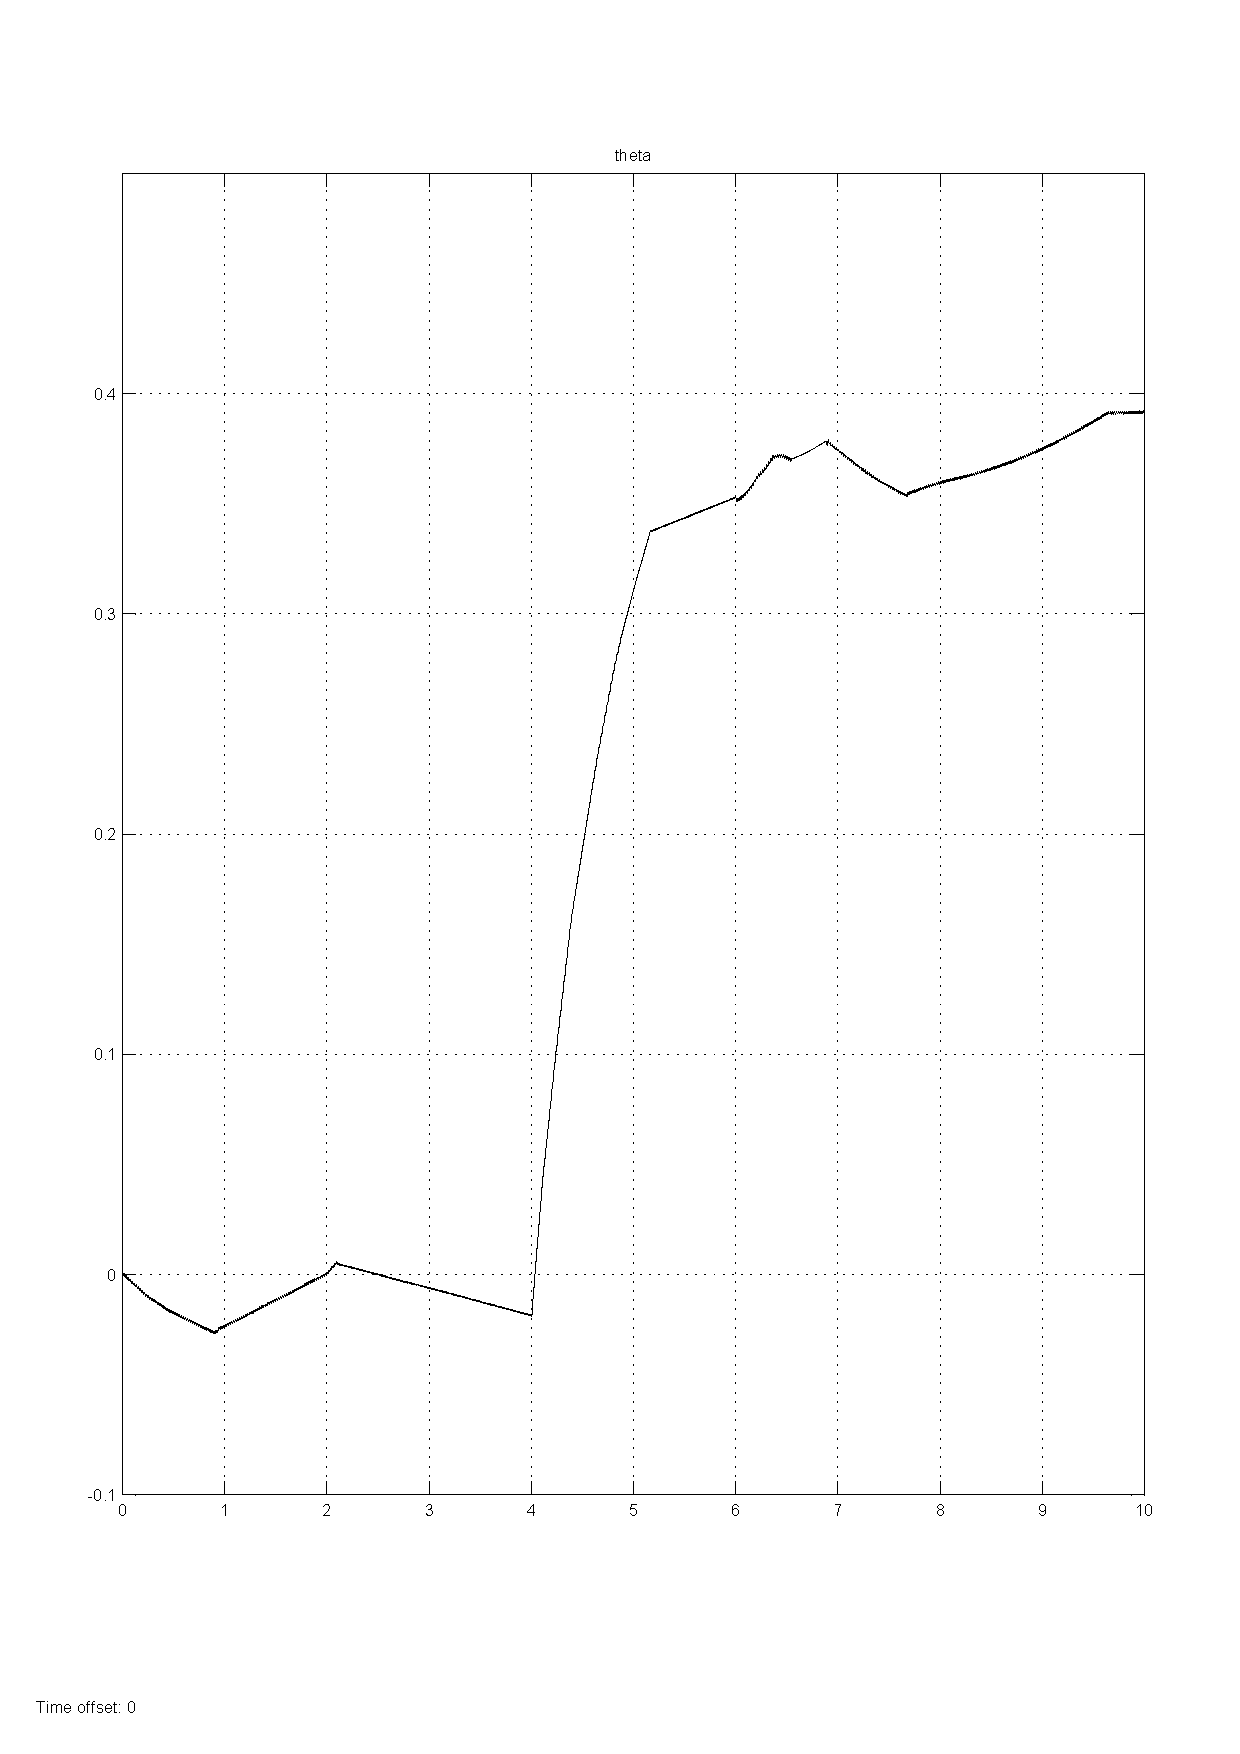
\includegraphics[width=0.8\textwidth]{03_Grafiken/theta_PID.pdf}
	\caption{Angle of theta using the PID controller}
	\label{fig:theta_PID}
\end{figure}

Figure \ref{fig:theta_PID} shows the angle of \textit{theta} after the whole sequence. It is the same as the angle of phi - the estimated angle is not hold stable and there are heavy influences at the time, the other two steps occur.

\begin{figure}
	\centering
		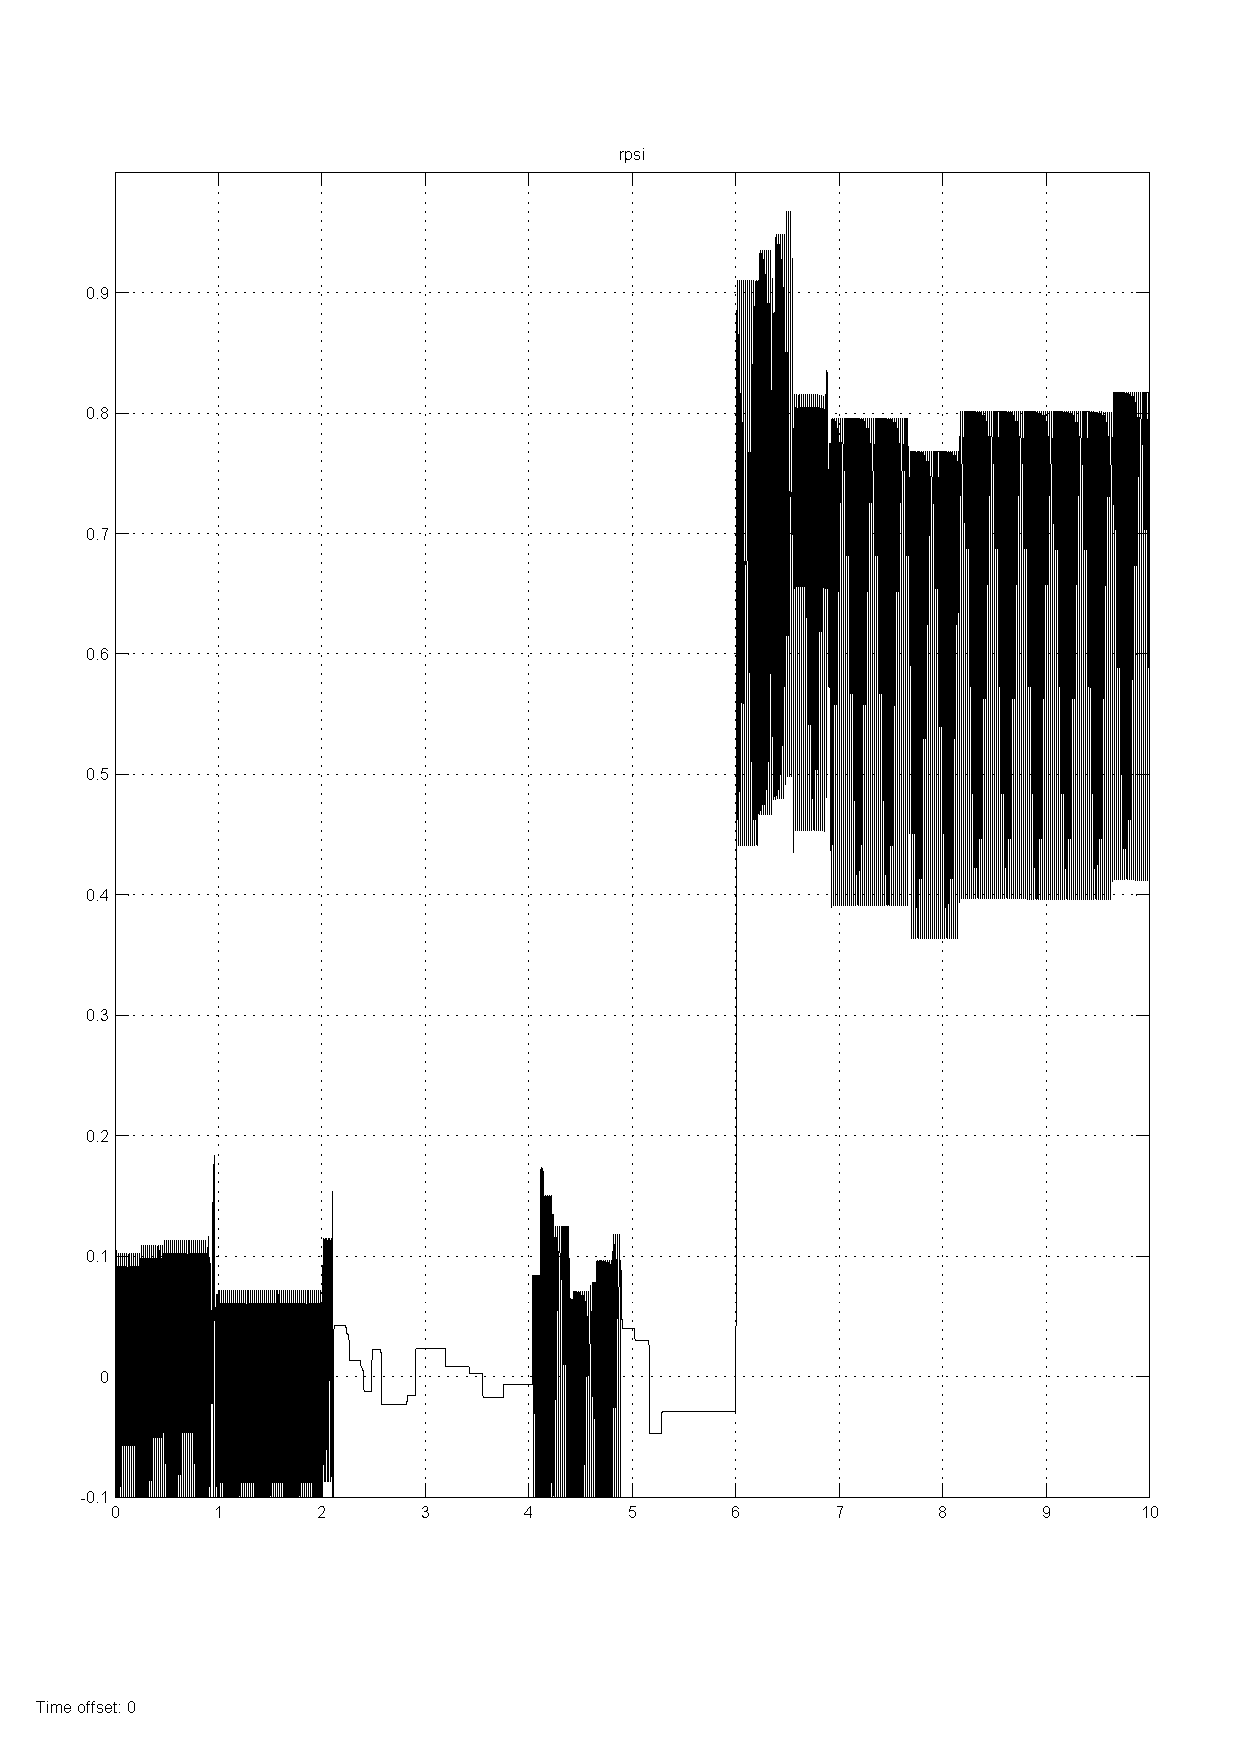
\includegraphics[width=0.8\textwidth]{03_Grafiken/rpsi_PID.pdf}
	\caption{Angular velocity of psi using the PID controller}
	\label{fig:rpsi_PID}
\end{figure}

Figure \ref{fig:rpsi_PID} shows the angular velocity of \textit{psi}, \textit{rpsi}, after the whole sequence. The rate is oscillating, but that is just the behavior of the simulation. In the real copter, the inertia of masses in movement prevents that.

The following figures are showing the same scopes, using the state space controller instead of the PID controller.

\begin{figure}
	\centering
		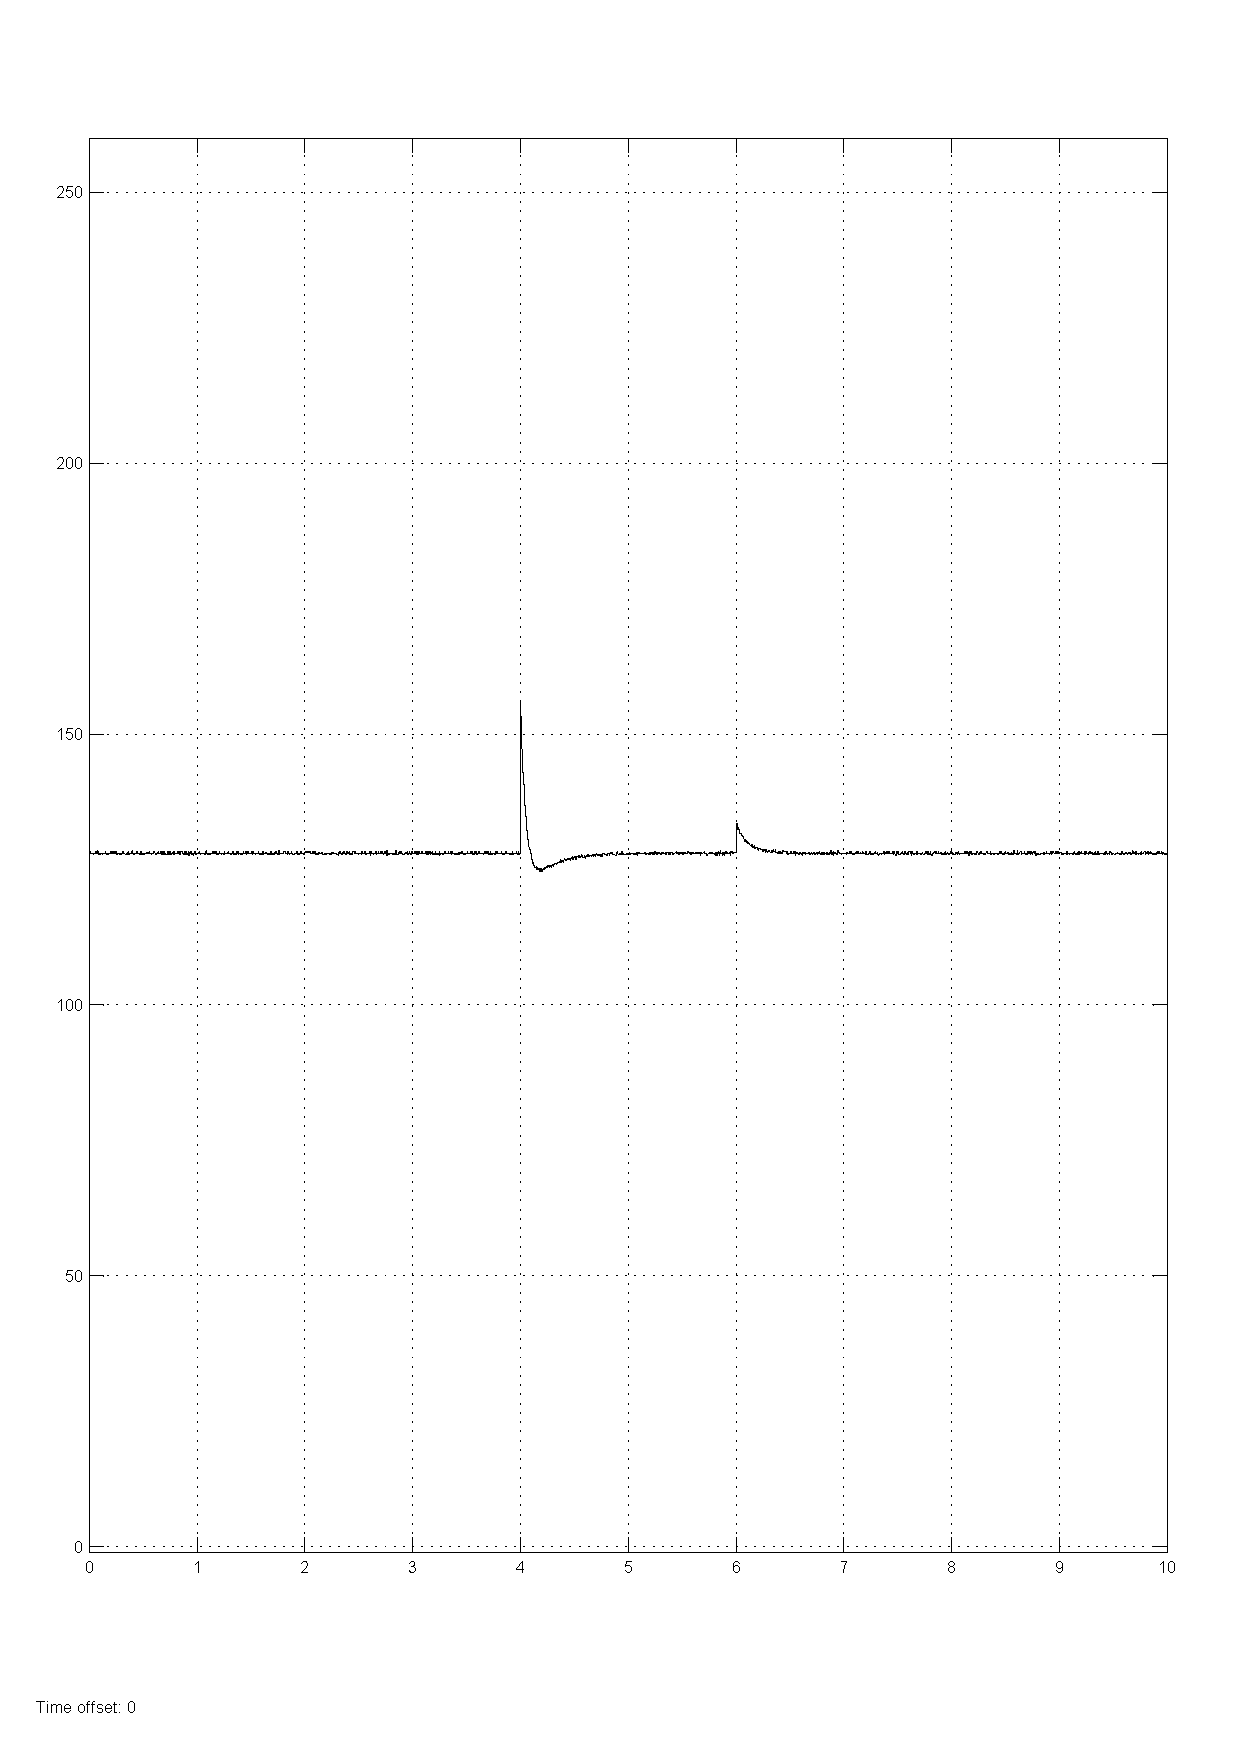
\includegraphics[width=0.8\textwidth]{03_Grafiken/Motor2_SS.pdf}
	\caption{Set value for one motor using the state space controller}
	\label{fig:Motor2_SS}
\end{figure}

In contrast to the PID controller, the state space controller does not push the actuating variables very high. There is just a little peak, at the moment the step occurs (Figure \ref{fig:Motor2_SS}).

\begin{figure}
	\centering
		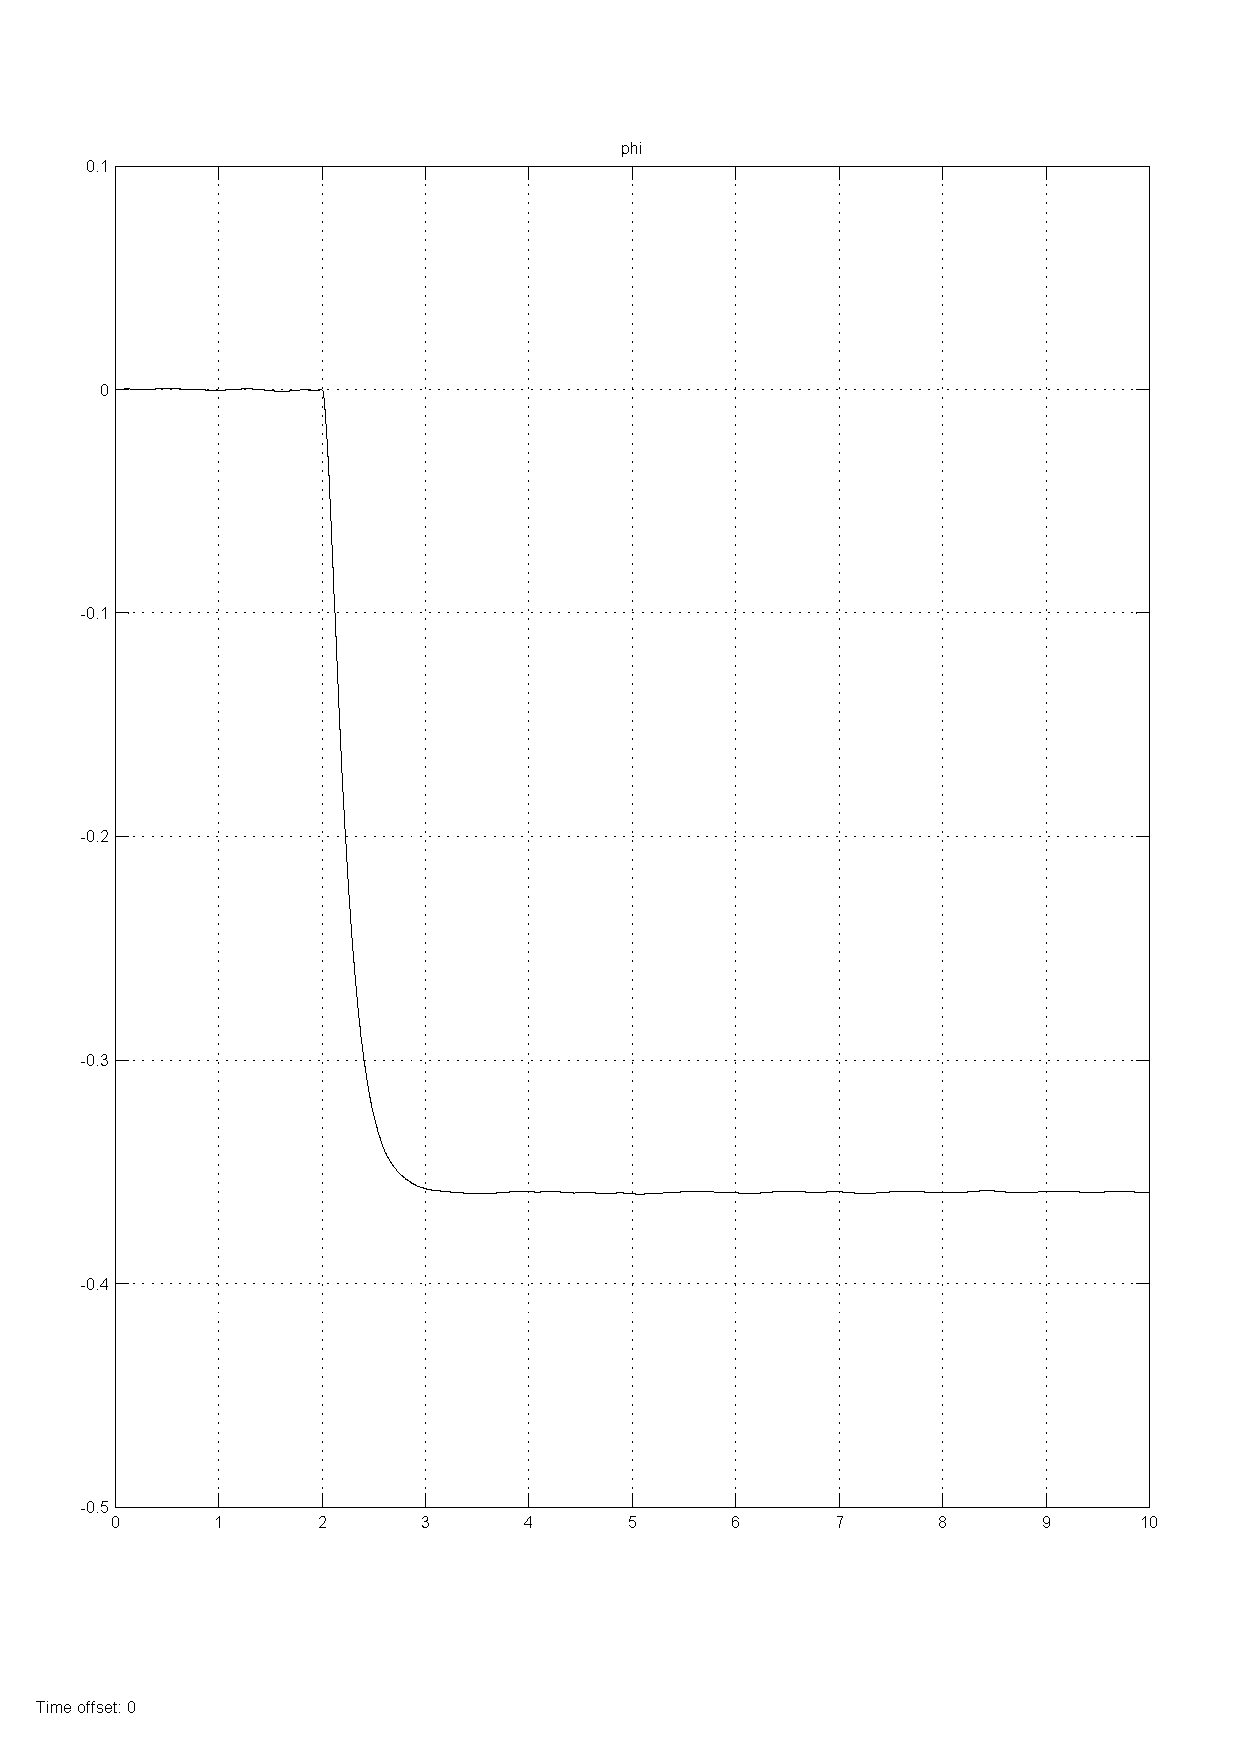
\includegraphics[width=0.8\textwidth]{03_Grafiken/phi_SS.pdf}
	\caption{Angle of phi using the state space controller}
	\label{fig:phi_SS}
\end{figure}

Figure \ref{fig:phi_SS} shows the angle of phi during the simulation. The estimated angle of -0.35 rad is reached within 0.5 seconds and is kept very accurate. Furthermore there is no influence of the other two steps at second four and second six.

\begin{figure}
	\centering
		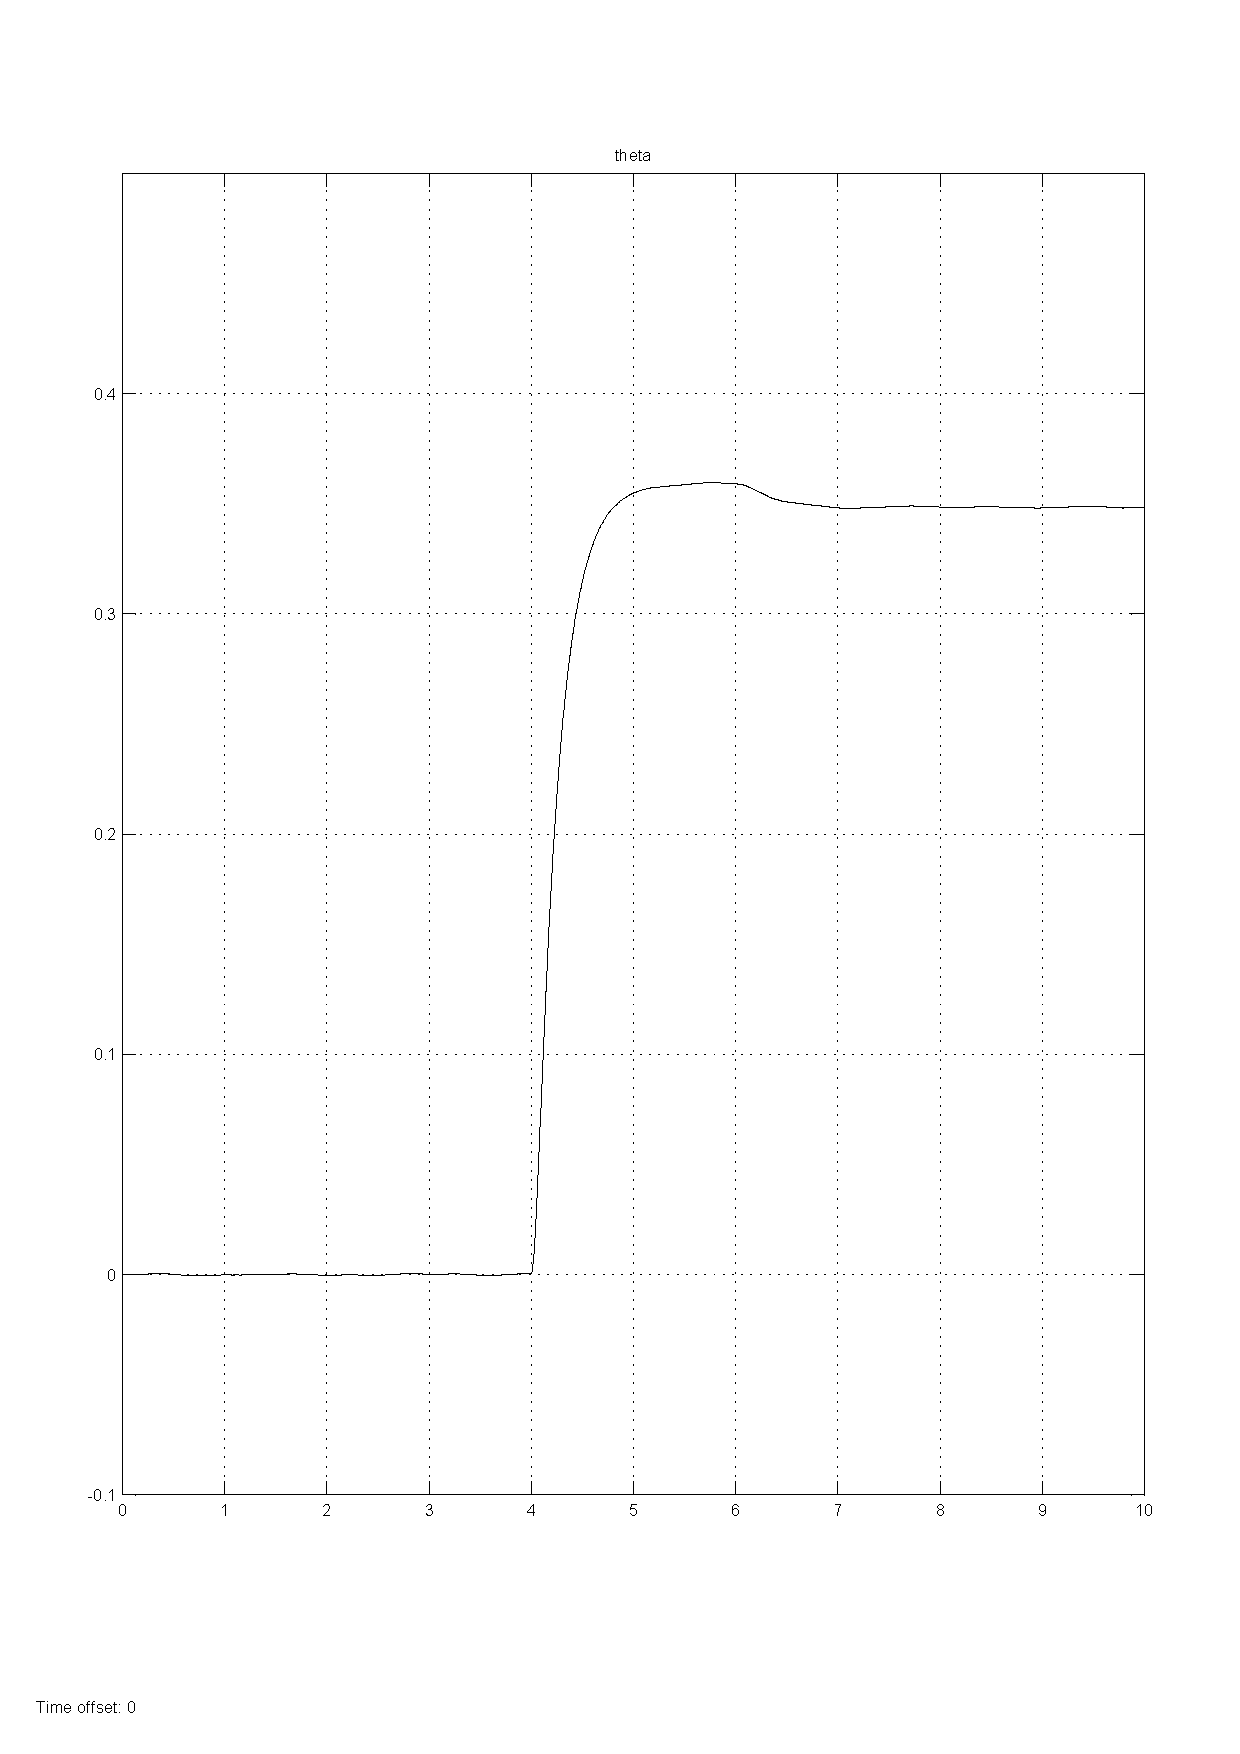
\includegraphics[width=0.8\textwidth]{03_Grafiken/theta_SS.pdf}
	\caption{Angle of theta using the state space controller}
	\label{fig:theta_SS}
\end{figure}

Figure \ref{fig:theta_SS} shows the angle of theta during the simulation. Like the angle of phi, the estimated angle of 0.35 rad is reached within 0.5 seconds. The step to the rate of psi at second six reduces the angle about approximately 0.015 rad, which is not even one degree and therefore insignificant small.

\begin{figure}
	\centering
		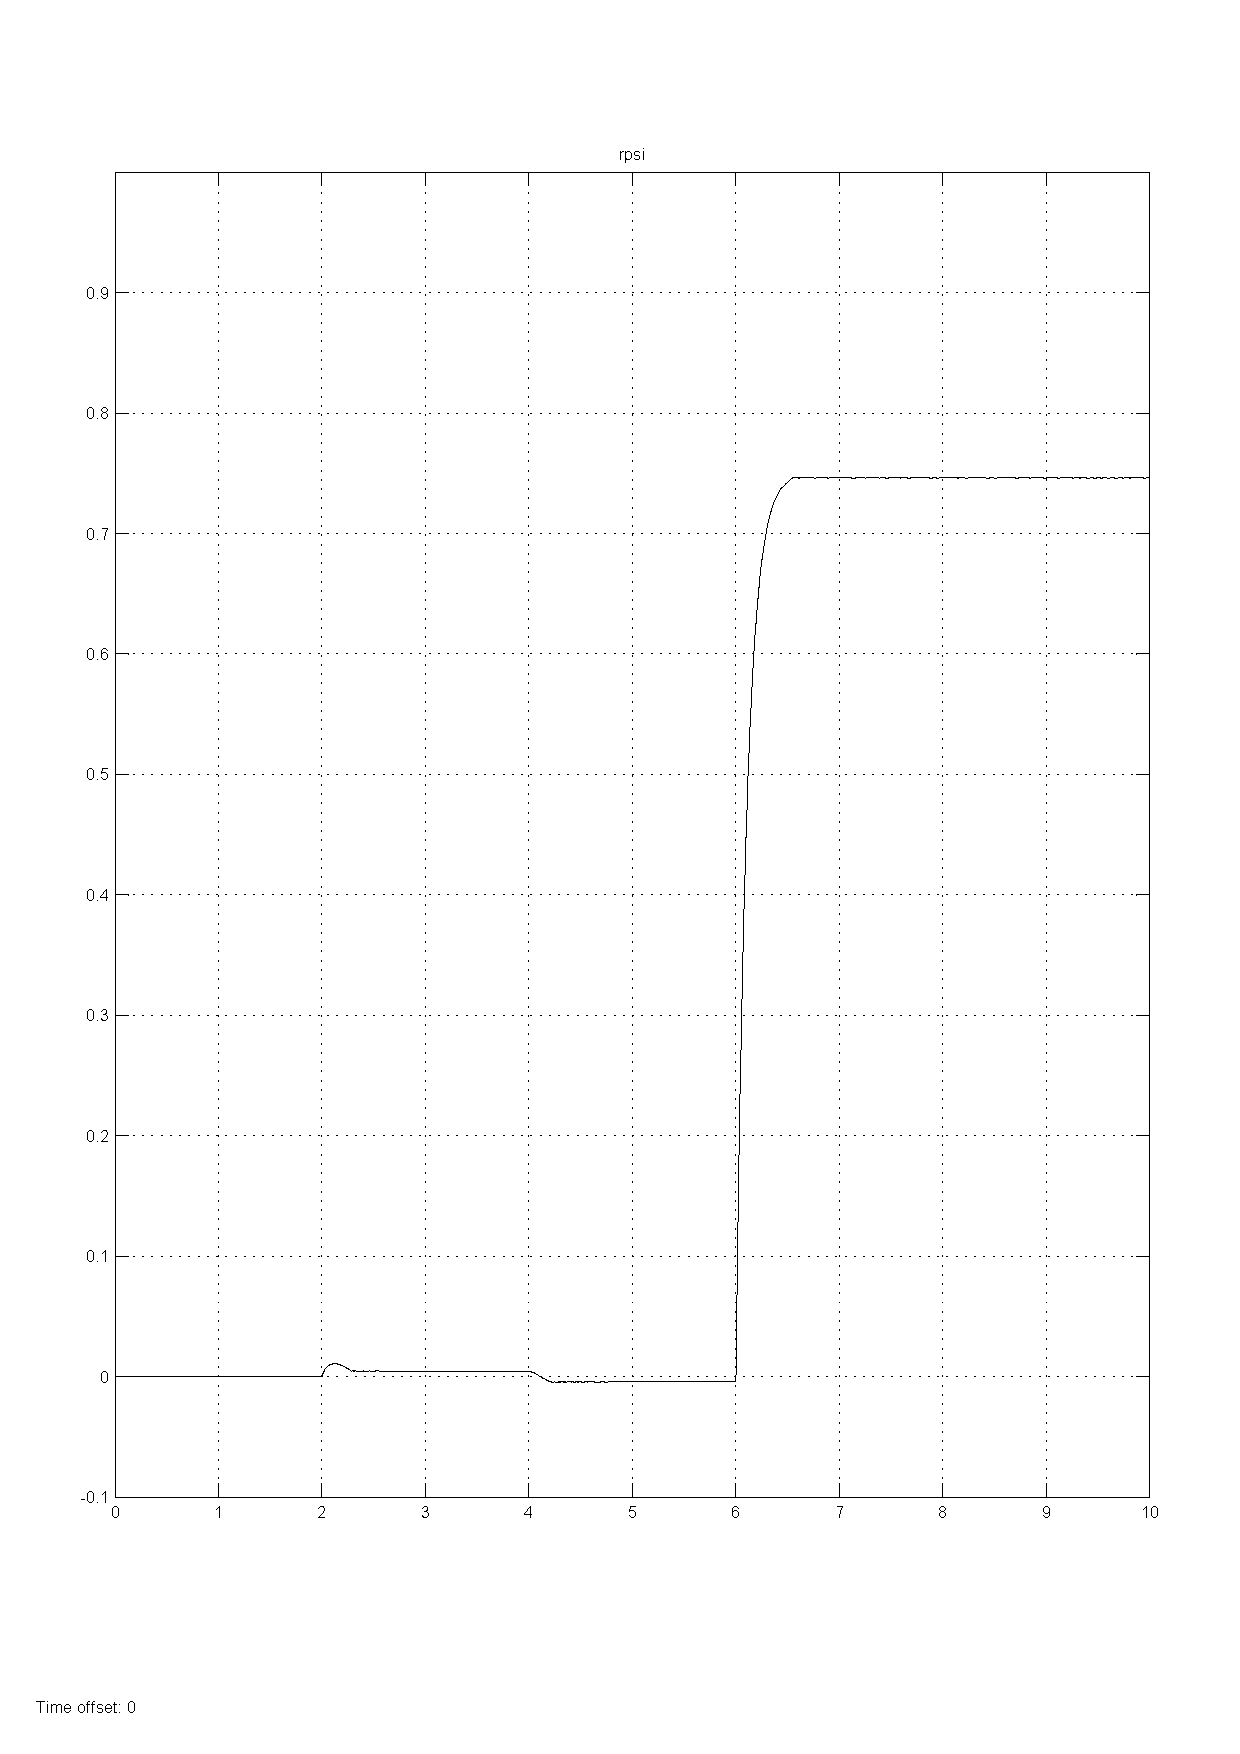
\includegraphics[width=0.8\textwidth]{03_Grafiken/rpsi_SS.pdf}
	\caption{Angular velocity of psi using the state space controller}
	\label{fig:rpsi_SS}
\end{figure}

Figure \ref{fig:rpsi_SS} shows the very fast and accurate behavior of the rate of psi. The rate is reached very fast within less than half a second.


All in all, the simulation of the developed state space controller went well, and the next step, the HIL tests, can be performed.

\pagestyle{fancy}
\subsection{Hardware In the Loop test}\label{chapter_HILTest}

After the successful tests of the Matlab/Simulink state space controller, the controller was implemented in C (chapter \ref{chapter_IMPLC}). In this step, the real quadrocopter including the controller is connected to the computer with the Matlab/Simulink model on it. The actuating variables are calculated by the real hardware and software in the quadrocopter. Unfortunately it was not possible to get a stable connection between the quadrocopter and the computer. So that part of the testing had to be skipped, after several days of trying to get the connection stable. Because of the good results with the simulation, it was possible to continue with the tests in the real quadrocopter without performing the Hardware In the Loop tests.

\pagestyle{fancy}
\subsection{Real quadrocopter test}\label{chapter_RealCopterTest}

As described in chapter \ref{chapter_HILTest}, the Hardware In the Loop tests did not work. So to test the new state space controller directly in the quadrocopter, the rotor blades were removed. Starting with the first test, everything went well. It was not possible to fly with the quadrocopter, but to travel on the ground. After several hours of parameter tuning, by moving the poles and adjusting the maximum angles, the quadrocopter seems to be able to fly. But to get a perfect behavior in the air, additional hours have to be spend in fine tuning.    % chapter about the testing (simulation & real copter)
\clearpage %neue Seite erzwingen

\pagestyle{fancy}
\section{Future prospects}\label{chapter_FUTUREPROSPECTS}

Although the state space controller works perfectly in the simulation, it is still necessary to spend some fine tuning to the controller in C. Also it is unknown, how the controller handles disturbances like wind. Maybe it is reasonable, to spend the state space controller a superimposed PI controller to avoid control deviation.\\
An other point of the future prospects is to reduce the number of sensors. A first try is to simply delete some sensors and readjust the state space controller. The second idea is to implement an observer to simulate some state variables in real time on the microcontroller.\\
Anyway - the goal of this student project is achieved and provides a basis for further quadrocopter projects. % chapter about the future :)
\clearpage %neue Seite erzwingen

\pagestyle{fancy}
\section{Appendix}\label{chapter_Appendix}

\subsection{State space controller C function}\label{chapter_CFUNC}
C source code for the state space controller:

\lstset{language=C}
\begin{lstlisting}
/*  Control function for the state space controller */
void Controll(CopterState* copterState, CopterConfig* copterConfig) 
{
    // KV-Factors:
    static float rpsi_rpsi = 1.62;
    static float rpsi_theta = -0.07;
    static float rpsi_phi = 0;

    static float theta_rpsi = 0;
    static float theta_theta = 2.65;
    static float theta_phi = 0;

    static float phi_rpsi = 0;
    static float phi_theta = 0;
    static float phi_phi = 1.86;

    // KR-Factors:
    static float rpsi_Rrpsi = 1.62;
    static float rpsi_Rtheta = 0;
    static float rpsi_Rphi = 0;
    static float rpsi_Rrphi = 0;
    static float rpsi_Rrtheta = 0.04;

    static float theta_Rrpsi = 1.01;
    static float theta_Rtheta = 2.65;
    static float theta_Rphi = 0;
    static float theta_Rrphi = 0;
    static float theta_Rrtheta = 3.53;

    static float phi_Rrpsi = 0;
    static float phi_Rtheta = 0;
    static float phi_Rphi = 1.86;
    static float phi_Rrphi = 2.79;
    static float phi_Rrtheta = 0;

    // Auxiliary variables
    float rpsi_SET, theta_SET, phi_SET; 
    float remote_Pitch_SS, remote_Roll_SS, remote_Yaw_SS;
    float theta_sens, rtheta_sens, phi_sens, rphi_sens, rpsi_sens;
    float M1, M2, M3, M4;
    float m_r_Pitch, m_r_Roll, m_r_Yaw;    
     
    // Motorvalues for the next sampletime
    static uint8 M1_limited = 0;
    static uint8 M2_limited = 0;
    static uint8 M3_limited = 0;
    static uint8 M4_limited = 0;

    // Set outputs to values calculated last sample time
    copterState->setpointFront = M1_limited;
    copterState->setpointLeft  = M2_limited;
    copterState->setpointRear  = M3_limited;
    copterState->setpointRight = M4_limited;

    // Calculate the remote input factors
    remote_Pitch_SS = ((float) copterState->remotePitch)/7;
    remote_Roll_SS = ((float) copterState->remoteRoll)/7;
    remote_Yaw_SS = ((float) copterState->remoteYaw)/3;

    // Calculate the sensor factors
    theta_sens = ((float) copterState->Pitch_filt)/2;
    phi_sens = ((float) copterState->Roll_filt)/2;
    rtheta_sens = ((float) copterState->angVelP)/220;
    rphi_sens = ((float) copterState->angVelR)/220;
    rpsi_sens = ((float) copterState->angVelY)/320;

    // Calculate the total input to each control branch
    rpsi_SET = remote_Yaw_SS * rpsi_rpsi + remote_Pitch_SS * theta_rpsi + remote_Roll_SS * phi_rpsi;
    theta_SET = remote_Yaw_SS * rpsi_theta + remote_Pitch_SS * theta_theta + remote_Roll_SS * phi_theta;
    phi_SET = remote_Yaw_SS * rpsi_phi + remote_Pitch_SS * theta_phi + remote_Roll_SS * phi_phi;

    // Calculate the new set values for the three branches
    m_r_Yaw = rpsi_SET - (rpsi_sens * rpsi_Rrpsi + theta_sens * rpsi_Rtheta + phi_sens * rpsi_Rphi - rphi_sens * rpsi_Rrphi + rtheta_sens * rpsi_Rrtheta);
    m_r_Roll = phi_SET - ( rpsi_sens * phi_Rrpsi + theta_sens * phi_Rtheta + phi_sens * phi_Rphi - rphi_sens * phi_Rrphi + rtheta_sens * phi_Rrtheta);
    m_r_Pitch = theta_SET - ( rpsi_sens * theta_Rrpsi + theta_sens * theta_Rtheta + phi_sens * theta_Rphi - rphi_sens * theta_Rrphi + rtheta_sens * theta_Rrtheta);

    // Calculate new setpoints of all motors
    M1 = (float)(copterState->remoteForceRaw) - m_r_Pitch + m_r_Yaw;
    M2 = (float)(copterState->remoteForceRaw) + m_r_Roll - m_r_Yaw;
    M3 = (float)(copterState->remoteForceRaw) + m_r_Pitch + m_r_Yaw;
    M4 = (float)(copterState->remoteForceRaw) - m_r_Roll - m_r_Yaw;

    // Saturate setpoint of Motor1 to 10 if less and 255 if above
    if(M1 < 10){
    M1_limited = 10;
    }else if(M1 > 255){
    M1_limited = 255; 
    }else{
       M1_limited=(uint8)(M1);
    }

    // Saturate setpoint of Motor2 to 10 if less and 255 if above
    if(M2 < 10){
      M2_limited = 10;
    }else if(M2 > 255){
      M2_limited = 255; 
    }else{
         M2_limited=(uint8)(M2);
    }

    // Saturate setpoint of Motor3 to 10 if less and 255 if above
    if(M3 < 10){
      M3_limited = 10;
    }else if(M3 > 255){
      M3_limited = 255; 
    }else{
         M3_limited=(uint8)(M3);
    }
    
    // Saturate setpoint of Motor4 to 10 if less and 255 if above
    if(M4 < 10){
      M4_limited = 10;
    }else if(M4 > 255){
      M4_limited = 255; 
    }else{                 
         M4_limited=(uint8)(M4);
    } 
}
\end{lstlisting}

\subsection{Quick Start Guide}\label{chapter_QSG}

Follow the steps below for quickly use and change the state space controller in MATLAB Simulink.

\begin{enumerate}
	\item Use Matlab version R2009b or higher
	\item Switch to directory 'StateSpaceController' in Matlab
	\item If necessary, change the poles in 'Test\_Reglerauslegung.m' (\textit{place} command)
	\item Run 'Test\_Reglerauslegung.m'
	\item feedback- and pre-intensification factors are calculated
	\item Switch to directory 'BasicProject' in Matlab
	\item Open 'System\_Design\_Quadrocopter.mdl' (this may take some time)
	\item Open the Control-block and make sure, the switches enable the state space controller
	\item Start the Simulation
\end{enumerate}

To adjust the controller in C:

\begin{enumerate}
	\item Open 'Project.mcp' in Metroworks Codewarrior
	\item Switch to the function 'Controll' in 'flightcontrol.c'
	\item Adjust the KR- and KV-factors according to the Matlab variables K\_ret and KV  
	\item Flash the new software to the quadrocopter
\end{enumerate}

 % chapter about the future :)
\clearpage %neue Seite erzwingen

% Literaturverzeichnis_einfach
% ****************************

\begin{thebibliography}{99}
\addcontentsline{toc}{section}{\refname}

% ------------------------------------------------------------------------------------------------------

%\bibitem{bib:TITEL intern}
%WOHER, \emph{Titel f�r Quelle}, ART der QUELLE, Aufruf: tt.mm.jjjj, \url{https://blubb.de}

\bibitem{bib:KULL}
Prof. Dr.-Ing. Hermann Kull, \emph{Kapitel 7, Zustandsregelung}, Systemtechnik 2 manuscript , summer term 2011, \url{http://www.hs-esslingen.de/de/mitarbeiter/hermann-kull}

\bibitem{bib:MASTERDOC}
Tommaso Bresciani, \emph{Modelling, Identification and Control of a Quadrotor Helicopter}, Department of Automatic Control Lund University, Version: October 2008, ISRN LUTFD2/TFRT--5823--SE

\bibitem{bib:LUNZE}
Jan Lunze, \emph{Regelungstechnik 2: Mehrgr��ensysteme, Digitale Regelung}, Springer Verlag, 5. Auflage, ISBN 978-3540784623

\bibitem{bib:UNBEHAUEN}
Heinz Unbehauen, \emph{Regelungstechnik II: Zustandsregelungen, digitale und nichtlineare Regelsysteme }, Vieweg+Teubner Verlag, 9. Auflage, ISBN 978-3528833480

% ------------------------------------------------------------------------------------------------------

\end{thebibliography} 
\clearpage %neue Seite erzwingen

\end{document}